\documentclass[a4paper,11pt,twoside,toc=listof]{scrbook}

% packages 
\usepackage{arsclassica}    % fancy layout
\usepackage[english]{babel}\addto{\captionsenglish}{\renewcommand{\bibname}{References}}
\usepackage{caption}         % figure captions
\usepackage[square,numbers,super,sort&compress]{natbib}  % bibliography style
\usepackage[cc]{titlepic}    % enable logo on title page
\usepackage{graphicx}       % logo related
\usepackage{standalone}

\usepackage{bm}
\usepackage{amsmath}

% thesis only
\usepackage[nottoc,notlof,notlot,notbib]{tocbibind}
\RequirePackage{titlesec}
\RequirePackage{soul}

% used in into
\usepackage{acronym}

% used in methods
\usepackage{array}
\usepackage{booktabs}
\newcolumntype{L}{>{\centering\arraybackslash}m{4cm}}
\definecolor{light-gray}{gray}{0.95}
\usepackage{bm}
\DeclareMathOperator*{\argmin}{arg\,min}
\usepackage{tikz-cd}
\usepackage{amssymb}

% predictive modelling 
\usepackage{multirow}

% appendices
\usepackage{pdfpages}
\usepackage{longtable}

% Margins for pretty version ::
%\usepackage[pass]{geometry}
% Margins for university regulations ::
\usepackage[top=2cm, bottom=4cm, left=4cm, right=2.5cm]{geometry}
\usepackage{setspace}
\onehalfspacing

% don't hang captions
\captionsetup{format=plain}

% bibliography
\bibliographystyle{thesis}

% title setup
\title{ \vspace{2in} Unravelling higher order chromatin organisation through statistical analysis \\ \vspace{2em} 
%\author{Benjamin L. Moore} 
Benjamin L. Moore \\
\date{} \vspace{3em}
{\normalsize Doctor of Philosophy \\ 
The University of Edinburgh \\ 2015 \\} %\vspace{5em}
}

\titlepic{\vspace{1in} 
\includegraphics[width=\textwidth]{/Users/benmoore/hvl/1yrReport/figs/igmm.png}}

%\usepackage{etoolbox}
% http://tex.stackexchange.com/questions/204974/how-to-change-the-appearance-of-listof-headers

%\newcommand{\hhff }{\sffamily\textls[80]{\scshape }}

% KOMA script fix
\def\bf{\normalfont\bfseries}

\begin{document}

\frontmatter

\maketitle
\clearpage

%\addcontentsline{toc}{chapter}{Declaration}
\chapter{Declaration}

\begin{quote}
This thesis presents my own work, wherever the contributions of others were involved this is clearly indicated. It has not been submitted for any other degree or professional qualification. 
\end{quote}

\hfill ---Benjamin L. Moore (2015)

\clearpage

%\addcontentsline{toc}{chapter}{Acknowledgements}
\chapter{Acknowledgements}

% Firstly, I must thank my supervisor Colin Semple for the many valuable discussions and ideas that guided this thesis. Thanks also to my secondary supervisor Stuart Aitken, an inexhaustible source of statistical expertise.

% On a personal note, it would be remiss of me not to thank my mother for her support during the past three years (not to mention the prior twenty-two). Finally, thank you Nika for the pep talks and good times along the way.

\clearpage

% ---------- Abstract ---------- %
%\addcontentsline{toc}{chapter}{Abstract}
\chapter{Abstract}
Recent technological advances underpinned by high throughput sequencing have given new insights into the three-dimensional structure of mammalian genomes. Chromatin conformation assays have been the critical development in this area, particularly Hi-C, which ascertains genome-wide patterns of intra and inter-chromosomal contacts. However many open questions remain concerning the functional relevance of such higher order structure, the extent to which it varies, and how it relates to other features of the genomic and epigenomic landscape.

Current knowledge of nuclear architecture describes a hierarchical organisation ranging from small loops between individual loci, to megabase-sized self-interacting topological domains (TADs), encompassed within large multimegabase chromosome compartments. In parallel with the discovery of these strata, the ENCODE project has generated vast amounts of data through ChIP-seq, RNA-seq and other assays applied to a wide variety of cell types, forming a comprehensive bioinformatics resource.

In this work we combine Hi-C datasets describing physical genomic contacts with a large and diverse array of chromatin features derived at a much finer scale in the same mammalian cell types. These features include levels of bound transcription factors, histone modifications and expression data. These data are then integrated in a statistically rigorous way, through a predictive modelling framework from the machine learning field. These studies were extended, within a collaborative project, to encompass a dataset of matched Hi-C and expression data collected over a murine neural differentiation timecourse.

We compare higher order chromatin organisation across a variety of human cell types and find pervasive conservation of chromatin organisation at multiple scales. We also identify structurally variable regions between cell types, that are rich in active enhancers and contain loci of known cell-type specific function. We show that broad aspects of higher order chromatin organisation, such as nuclear compartment domains, can be accurately predicted in a variety of human cell types, using models based upon underlying chromatin features. We dissect these quantitative models and find them to be generalisable to novel cell types, presumably reflecting fundamental biological rules linking compartments with key activating and repressive signals. These models describe the strong interconnectedness between locus-level patterns of local histone modifications and bound factors, on the order of hundreds or thousands of basepairs, with much broader compartmentalisation of large, multi-megabase chromosomal regions.

Finally, boundary regions are investigated in terms of chromatin features and co-localisation with other known nuclear structures, such as association with the nuclear lamina. We find boundary complexity to vary between cell types and link TAD aggregations to previously described lamin-associated domains, as well as exploring the concept of super-boundaries that span multiple levels of organisation. Together these analyses lend quantitative evidence to a model of higher order genome organisation that is largely stable between cell types, but can selectively vary locally, based on the activation or repression of key loci.

\cleardoublepage

%\addcontentsline{toc}{chapter}{Lay summary}
\chapter{Lay summary}

Each human cell contains DNA that would extend for two metres if fully straightened. Instead, this same length of DNA is highly compacted into micrometre-sized cell nuclei. Recently experimental methods such as Hi-C have been developed which allow the inspection of this folded state, generating counts of how frequently chromosomal regions are interacting with each other. These counts can be statistically analysed to reveal different levels of structures, including loops between two distant locations, knot-like domains of self-interacting regions, and broad stretches of mostly active or inactive regions. 

In this work, we bring together Hi-C datasets from several different publications and combine these with a large number of chromatin datasets that quantify, for example, levels different DNA-binding proteins as well as modifications to DNA packing histone proteins. We used these datasets to build predictive models of active and inactive states across each human chromosome in three different cell types, and achieved high predictive accuracy. We then compare and contrast these models, and use them to identify the key features which define active and inactive states. 

We also analyse the boundaries between domains and compare these across cell types. We find the domains themselves are highly conserved between cell types, but observe different chromatin features marking domain boundaries. Further collaborative work involved analysis of boundaries from Hi-C data taken over successive time points, where boundary markings were found to persist as cells differentiate from stem cells.

Overall we find the three-dimensional DNA structures within cells are highly similar even between human embryonic stem cells and cells derived from blood. Where there are differences, these areas tend to highlight biological activity specific to that cell type.

\clearpage

\chapter{Contents}

\makeatletter
\@starttoc{toc}
\makeatother
%\tableofcontents
\clearpage

\chapter{List of figures}

\makeatletter
\@starttoc{lof}% Print List of Figures
\makeatother
%\listoffigures
\clearpage

\chapter{List of tables}

\makeatletter
\@starttoc{lot}% Print List of Figures
\makeatother
%\listoftables
\clearpage

% ---------- Acronyms ---------- %
%\addcontentsline{toc}{chapter}{List of Acronyms}
\chapter{List of acronyms}

% this is auto-populated from csv (above)
\begin{acronym}[chromatin] % give longest one to fix width
\acro{3C}{Chromsome conformation capture (derivatives: 4C, 5C, Hi-C)}
\acro{AUROC}{Area under the receiver operating characteristic}
\acro{CAGE}{Cap analysis of gene expression}
\acro{ChIP-seq}{Chromatin immunoprecipitation following by high-throughput sequencing}
\acro{DI}{Directionality index}
\acro{ENCODE}{The encyclopaedia of DNA elements}
\acro{ESC}{Embryonic stem cell}
\acro{FDR}{False discovery rate}
\acro{FISH}{Flurorescent \emph{in-situ} hybridisation}
\acro{GC}{Guanine and cytosine (content of a DNA sequence)}
\acro{GO}{Gene ontology}
\acro{Hi-C}{Genome-wide 3C experiment using high-throughput sequencing}
\acro{HMM}{Hidden Markov Model}
\acro{ICE}{Iterative correction and eigenvector expansion}
\acro{IF}{Interaction frequency}
\acro{LAD}{Lamin associated domain}
\acro{MAD}{Median absolute deviation}
\acro{MSE}{Mean squared error}
\acro{NAD}{Nucleolus associated domain}
\acro{OOB}{Out-of-bag}
\acro{PCC}{Pearson correlation coefficient}
\acro{PCR}{Polymerase chain reaction}
\acro{PLS}{Partial least squares}
\acro{RF}{Random Forest}
\acro{RMSE}{Root mean-squared error}
\acro{RVS}{Regions of variable structure}
\acro{SHH}{Sonic Hedgehog}
\acro{TAD}{Topologically-associating domains}
\acro{TSS}{Transcription start site}
\acro{ZRS}{Zone of polarising activity regulatory sequence}
\end{acronym}
\clearpage

% ---------- Published ---------- %
%\addcontentsline{toc}{chapter}{Published material}
\chapter{Published material}

Some materials contained in this thesis have previously been published in:

\begin{quote}
Moore BL, Aitken S and Semple CA (2015) Integrative modeling reveals the principles of multi-scale chromatin boundary formation in human nuclear organization. \emph{Genome Biology}, {\bf 16}:100. \\ doi:\href{http://dx.doi.org/10.1186/s13059-015-0661-x}{10.1186/s13059-015-0661-x}
\end{quote} 

{\flushleft Parts of Section \ref{sec:metatads} are used in a submitted manuscript:}

\begin{quote}
Fraser J, Ferrai C, Chiariello AM, Schueler M, Rito T, Laudanno G, Barbieri M, Moore BL, Aitken S,
Morris KJ, Itoh M, Kawaji H, Jaeger I, Hayashizaki Y, Carninci P, Forrest ARR, FANTOM Consortium, Semple CA, Dostie J, Pombo A, Nicodemi M (2015) Hierarchical organization
of chromosome folding and its re-organization underlies transcriptional
changes in cellular differentiation. \emph{Submitted}
\end{quote}

\clearpage

% switch to actual page numbering
\mainmatter

% ---------- Intro ---------- %
\documentclass[a4paper,11pt,oneside]{book}

% packages 
\usepackage{arsclassica}    % fancy layout
\usepackage[english]{babel}\addto{\captionsenglish}{\renewcommand{\bibname}{References}}
\usepackage{caption}         % figure captions
\usepackage[square,numbers,super,sort&compress]{natbib}  % bibliography style
\usepackage[cc]{titlepic}    % enable logo on title page
\usepackage{graphicx}       % logo related

\usepackage{standalone}
\standalonetrue

% Margins for pretty version ::
%\usepackage[pass]{geometry}
% Margins for university regulations ::
\usepackage[top=2cm, bottom=4cm, left=4cm, right=2.5cm]{geometry}
\usepackage{setspace}
\onehalfspacing

% don't hang captions
\captionsetup{format=plain}

% bibliography
\bibliographystyle{../thesis}

% title setup
\title{ \vspace{3in} Unravelling higher order genome organisation {\small [working
    title]} \\ \vspace{2em} {\large {\bf Introduction}} }
\author{Benjamin L. Moore}
\titlepic{\vspace{2.2in} 
\includegraphics[width=\textwidth]{/Users/benmoore/hvl/1yrReport/figs/igmm.png}}

\begin{document}

%\maketitle

\chapter{Introduction}
\section{Genome organisation}\label{intro:genomeorg}
%
It's oft-stated that the DNA within each human cell would extend for two metres fully extended. Instead that same length of DNA packs into a cell nucleus with a diameter in the order of micrometers ($\mu$m). This is achieved through a complex organisation hierarchy, ranging from how chromosomes are arranged in the nucleus in territories, to nuclear interactions with the nucleolus or periphery, down to how DNA is wrapped around nucleosomes (for recent reviews, see \citenum{Pombo2015, Fraser2015}). While the biophysics of the latter level of organisation may be well understood, more broadly there is much still to learn about the guiding principles and functional importance of higher order chromatin organisation.

This introductory section will describe the current state-of-the-art in chromosome conformation capture experimental methods, as well as criticisms and considerations when interpreting these data, and discuss what is currently understood or theorised about the structure and function of higher order genome organisation. We compare competing models which attempt to recapitulate mechanisms of chromatin folding, and also explore some of the best understood organisational strata in mammalian higher order genome organisation.

%
%Briefly, DNA exists mostly as a left-handed double-helix of hydrogen bonded purines and pyrimidines. These in turn are wrapped around histone octamers, proteins with tuneable DNA packing properties. These wrapped histones can be visualised as "beads on a string" in transcriptionally active regions, and possibly as a more-compact 30 nanometre fibre, though this is disputed.\cite{Naumova2013} %citations therein

\subsection{C-methods and Hi-C}

Classical studies of chromosome conformation relied on microscopy techniques to visualise nuclear architecture, most commonly fluorescence \emph{in situ} hybridisation (FISH). These techniques led to the discovery of ``chromosome territories", regions of the nucleus wherein distinct chromosomes were thought to occupy, and more broadly identified the non-random arrangement of loci in three-dimensional space.\cite{DeWit2012, VanSteensel2010} Finer details of chromatin organisation, such as the proposed 30 nm fibre, were also introduced through microscopy-based techniques. Techniques such as FISH are powerful for precise inspection of single genes, but are low-throughput and offer limited resolution.\cite{DeWit2012}

With the advent DNA sequencing technology, new experimental methods emerged. Chromosome conformation capture (3C), introduced by Dekker \emph{et al.}\cite{Dekker2002} was the first sequencing-based method of assaying nuclear architecture. The method uses formaldehyde to cross-link nuclear proteins in place, trapping genomic regions that were physically co-located through bound proteins, then to apply a frequent restriction enzyme to shear the sample into fragments. Next, under dilute conditions, DNA fragments are ligated together. The dilute conditions favour ligations between fixed fragments, with the aim of generating hybrid fragments form two genomic regions which were close together in the original preparation. Cross-linking can then be reversed and, in the case of the original 3C method, measured by quantitative PCR using pre-designed primers for your fragments of interest. The end result is a relative measure of interaction frequency between any two regions of interest, in theory directly proportional to their distance in three-dimensional space.

The rapid advancement of sequencing, allowed the original 3C method to be further developed, first through microarray technology, then using high-throughput sequencing. Two protocols were proposed for a 3C-inspired one-to-many assay\cite{Zhao2006, Simonis2006} (both named 4C), whereby interactions were measured for a specific ``viewpoint" fragment against all other restriction fragments genome-wide. The same year a many-to-many assay (5C) allowed measurements for all restriction fragments within a specified region.\cite{Dostie2006} 

The final step was an all-versus-all assay, capable of assaying pairwise interaction frequencies between all restriction fragments of a genome. This assay was published by Lieberman Aiden \emph{et al.}\cite{Lieberman2009} and named Hi-C (Fig. \ref{fig:hicmethod}). The Hi-C method added biotin tagging to pull-down only ligated fragments for sequencing. At the time of publication, resolution of Hi-C data for analysis was limited by sequencing depth, given the huge number of restriction fragments produced by a 6-cutter enzyme (HindIII and NcoI were used in \cite{Lieberman2009}) but the falling costs of sequencing and proven utility of the assay meant subsequent Hi-C papers incrementally increased their sequencing depth, to a point where analysis could be performed at the level of individual restriction fragments, genome-wide.\cite{Dixon2012,  Selvaraj2013a, Jin2013, Rao2014}

\begin{figure}
\begin{center}
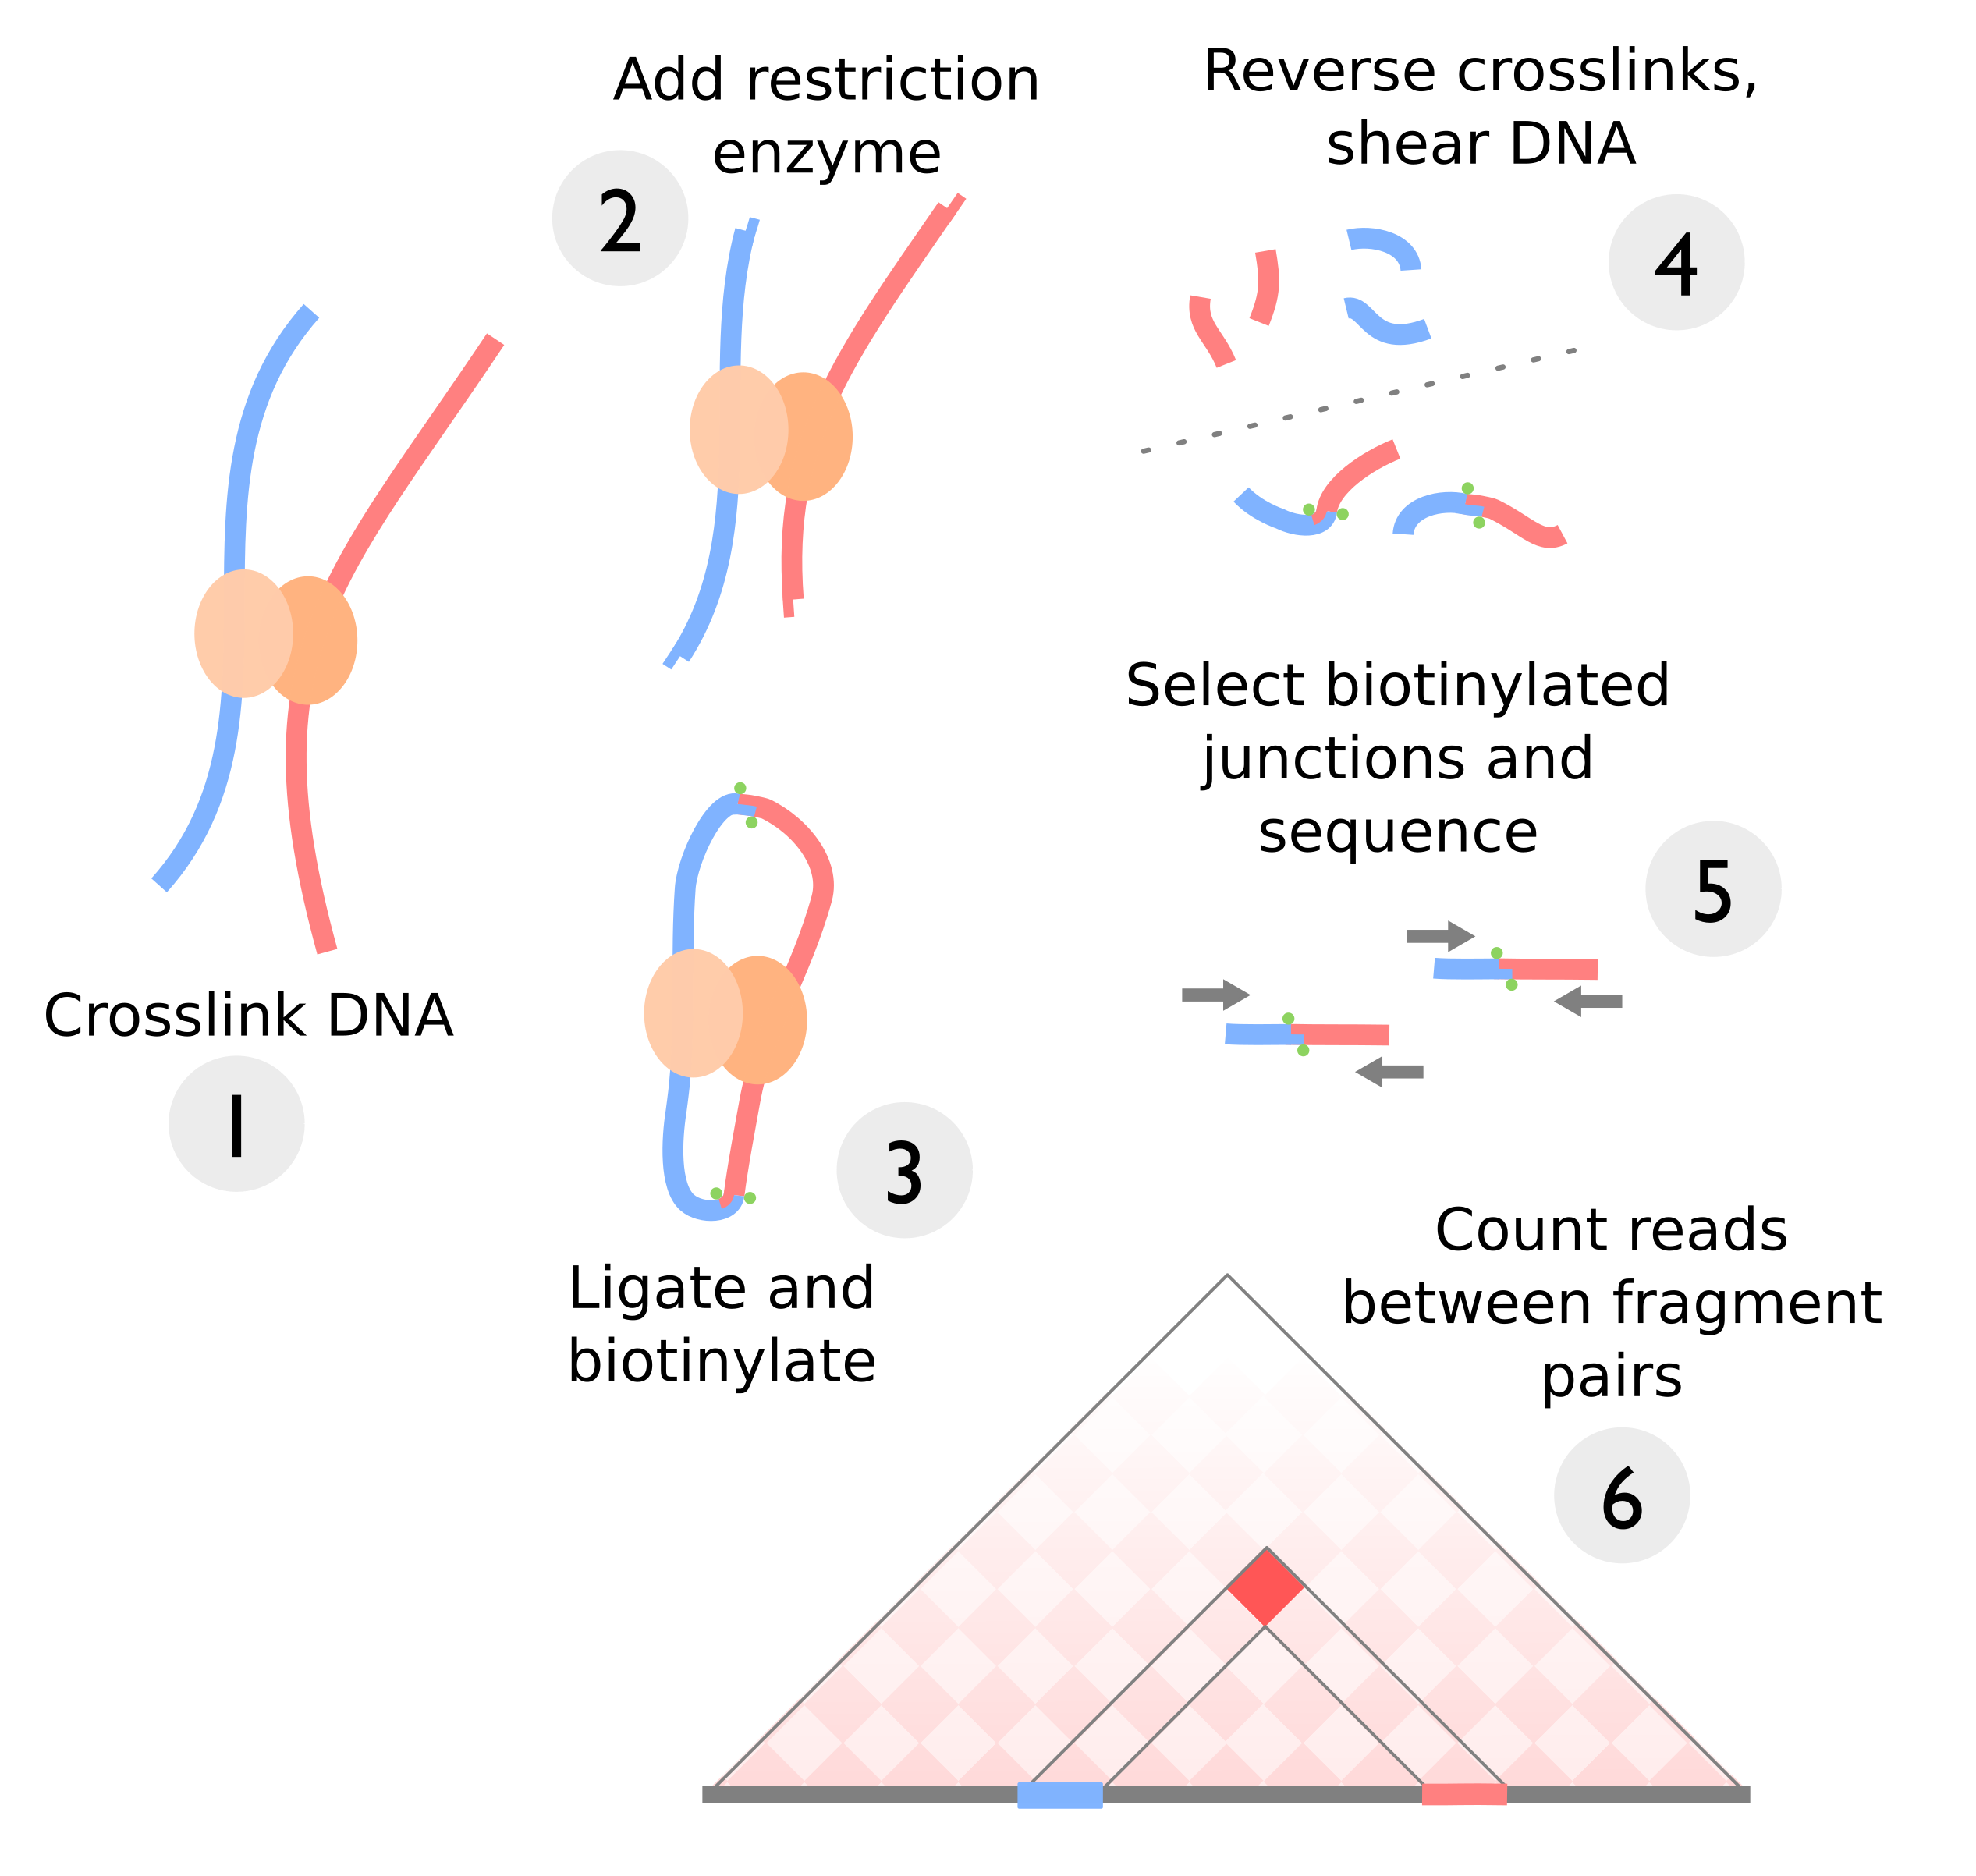
\includegraphics[width=4in]{figs/hic.png}
\captionsetup{width=\textwidth}
\caption[Steps in the Hi-C assay.]{ {\bf Steps in the Hi-C assay. } 
  Schematic of the Hi-C experimental procedure as described in Lieberman Aiden \emph{et al.}\cite{Lieberman2009}
}\label{fig:hicmethod}
\end{center}
\end{figure} 

\subsection{Hi-C variants}\label{sec:hicvar}

The interaction maps produced by Hi-C were found to exhibit several inherent biases. Fragment properties, such as their length, GC content and mappability, were confounding interaction frequency estimates and therefore needed to be normalised-away before subsequent analysis.\cite{Yaffe2011, Hu2013} A range of statistical techniques were developed to correct for these latent variables,\cite{Imakaev2012, Dekker2013, Hu2012, Li2014} while experimentalists instead looked to improve on the experimental procedure itself.

Tethered chromosome capture (TCC)\cite{Kalhor2012} was the first attempt to increase the signal to noise ratio of Hi-C contacts. In this method, ligations take place on a fixed surface, with the aim of preventing spurious ligations between fragments in solution which were not cross-linked. Kalhor \emph{et al.}\cite{Kalhor2012} reported a large decrease in observed interchromosomal contacts in their tethered library, suggesting many of those originally observed were caused by spurious ligation of non-crosslinked fragments.

Hi-C is a population-level assay, as the retrieved interaction counts are from a huge number of different cells. As well as building population-averaged models of genome structure, it is also of interest to probe cell-to-cell variability through single-cell approaches. For instance, it's been estimated that long-range contacts identified with C-methods may occur in as few as $10\%$ of cells at any one time.\cite{VanSteensel2010} 

In the first single-cell Hi-C study, Nagano \emph{et al.}\cite{Nagano2013} aimed to explore this cell-to-cell variability by performing the Hi-C assay on single, hand-selected nuclei. An obvious limitation this Hi-C variant is that a single restriction fragment can ligate to at most one other fragment, meaning even if $100\%$ yield were to be achieved, any $n \times n$ restriction fragment interaction matrix could at most populate $\frac{n}{2}$ cells; in practice, the realised yield of this first single cell Hi-C experiment was just $2.5\%$.\cite{Nagano2013} Nevertheless, single-cell Hi-C was able to reproduce findings from population-based (or ``ensemble") Hi-C, such as preferential interactions between active domains, but also was able to dissect \emph{trans} interactions, suggesting high cell-to-cell variability leads to their relatively uniform appearance in normal Hi-C interaction maps.\cite{Nagano2013} Combined with observations from TCC which gave evidence that interchromosomal contacts were disproportionately the result of spurious ligation,\cite{Kalhor2012} the functional significance of these \emph{trans} interactions seems at best unclear in the general case.

Capture-C is a C-method variant which attempts to address resolution problems associated with the Hi-C genome-wide pairwise assay by enriching for functional interactions using \emph{a priori} selection of target loci.\cite{Hughes2014} Indeed, a suggestion in the original Hi-C paper was that resolution could be improved by either increased sequencing or using hybrid capture.\cite{Lieberman2009} Since then, Hi-C variants with a target enrichment step have been developed, including Capture Hi-C (CHi-C)\cite{Dryden2014} and HiCap.\cite{Sahlen2015} These methods have been applied to genome-wide target sets (e.g. CHi-C assayed $22,000$ human promoters\cite{Mifsud2015}) and so it could be said that they are to Hi-C as exome-capture is to a whole-genome sequencing, in the contexts of conformation capture and variant discovery respectively. 

%Use of a cell population also averages away cell-cycle effects, with the vast majority of results coming from cells during interphase (around $97\%$\cite{Naumova2013}). Naumova \emph{et al.}\cite{Naumova2013} looked to assay chromosome conformation specifically over different cell cycle stages, to better understand chromosome compaction during mitosis.

\emph{In-situ} Hi-C was a recent refinement of the Hi-C method, from the publisher of the original method.\cite{Rao2014} The principle difference is that fixation and ligation now happen in place, within intact cell nuclei.

% DNase Hi-C

\subsection{Chromosome compartments}\label{sec:compartments}

In the paper describing the Hi-C technique,\cite{Lieberman2009}  Lieberman-Aiden \emph{et
  al.} described low-resolution structures they name  ``A'' and ``B'' nuclear compartments. These are regions with a median size of around 5 megabases which showed properties typical
of euchromatin and heterochromatin, respectively. A compartments were observed through 3D-FISH to be centrally-positioned in the nucleus and  ChIP-seq data showed several hallmarks of transcriptional activity. B compartments, conversely, were heterochromatic and lamina-associated regions, with little transcription and repressive histone modifications such as H3k9me3.\cite{Lieberman2009, DeWit2012} As expected from positioning data, the co-location of compartment types is also visible in their contact maps. 

\begin{figure}
\begin{center}
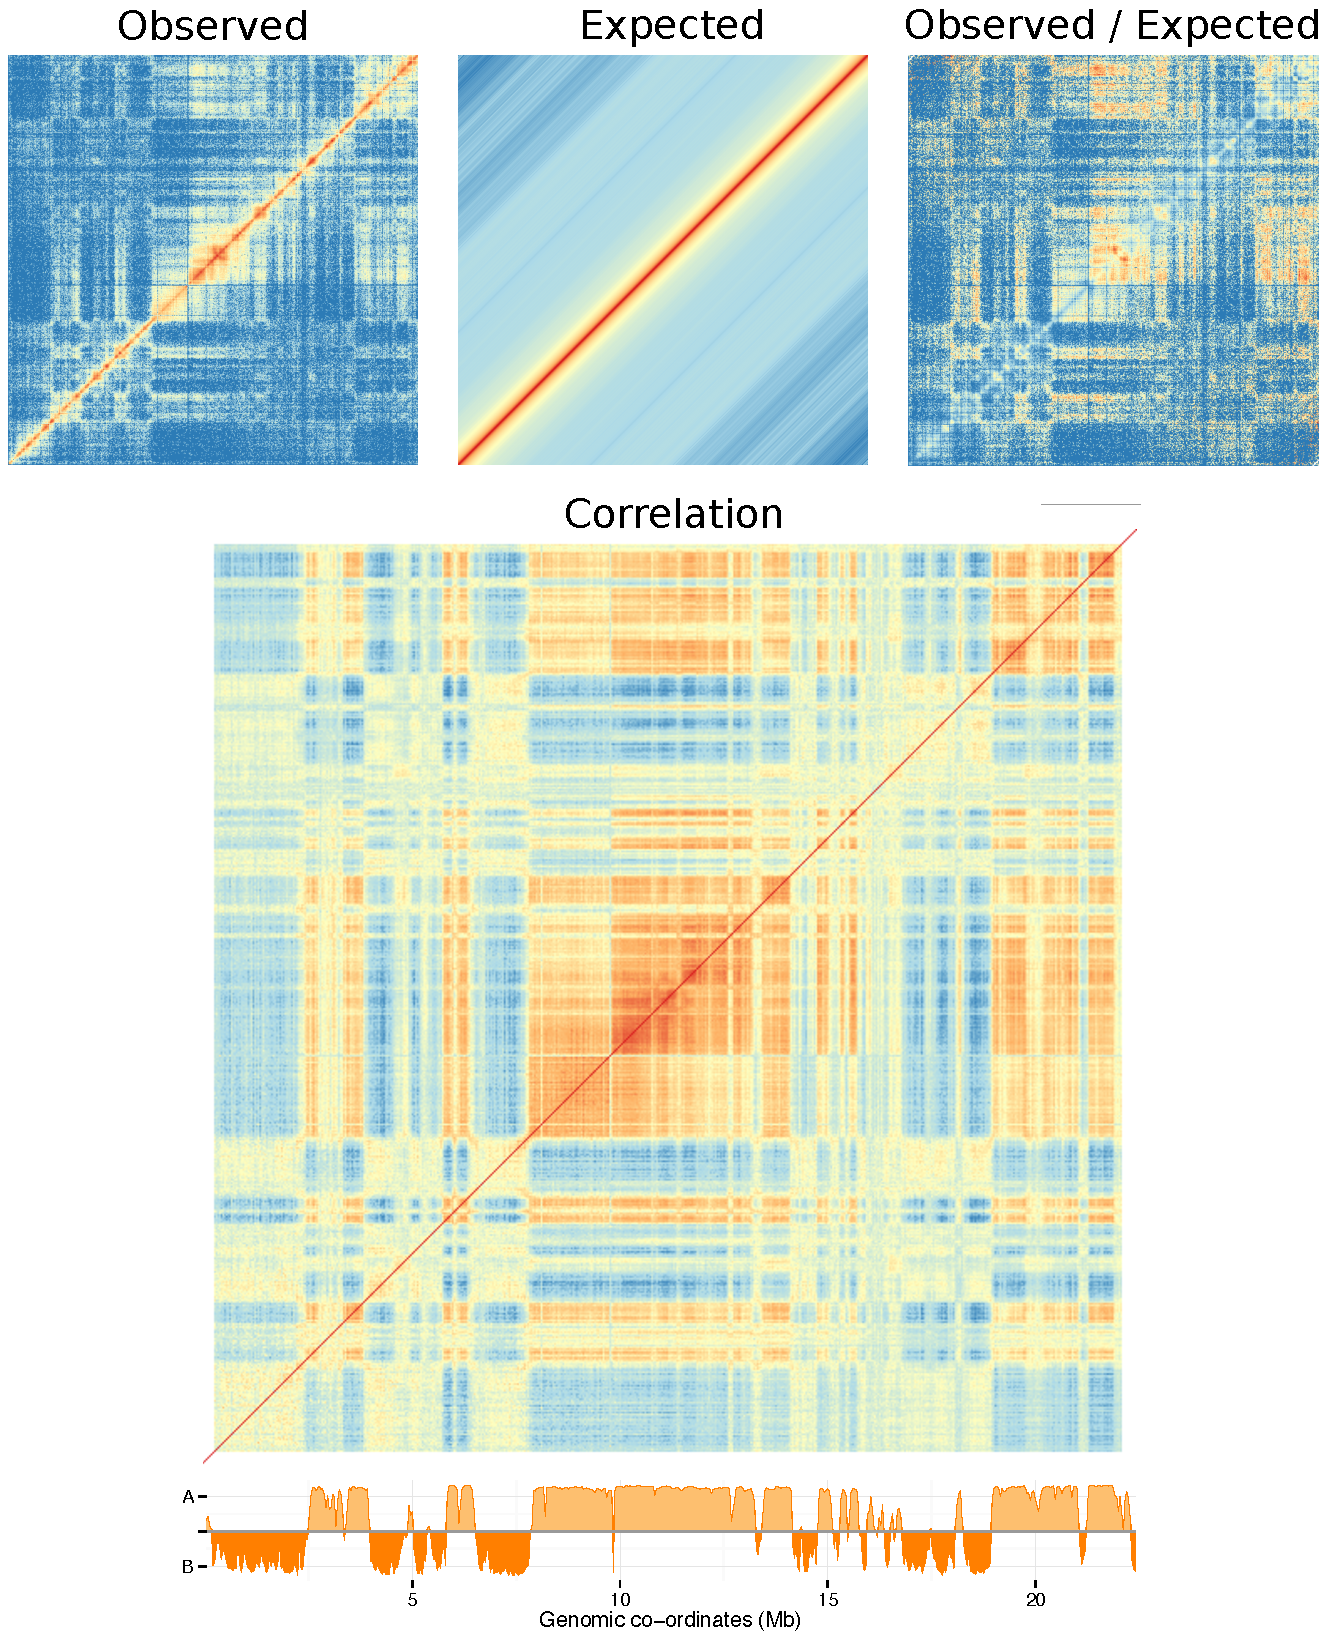
\includegraphics[width=.75\textwidth]{figs/eigcalc.png}
\captionsetup{width=\textwidth}
\caption[Derivation of A/B compartment profile from Hi-C data.]{ {\bf Derivation of A/B compartment profile from Hi-C data.} 
Observed interaction frequencies (O) are averaged along super-diagonals to give a distance-normalised expected matrix (E). The Pearson correlation of the O/E matrix then can undergo eigenvector expansion; in most cases eigenvector $\mathbf{v}$ with the largest eigenvalue, $\lambda$, then reflects A/B compartmentalisation.\cite{Lieberman2009}
}\label{fig:eigcalc}
\end{center}
\end{figure} 

These compartments were identified through a continuous eigenvector profile, derived from a normalised Hi-C contact matrix\cite{Lieberman2009} (Fig. \ref{fig:eigcalc}). This approach can be intuitively understood as formulated by \citet{Lajoie2014}:
\begin{enumerate}
\item A tartan pattern on normalised Hi-C matrices indicates two preferentially-contacting compartments (Fig. \ref{fig:eigcalc}).
\item Assume a function ($c$) that maps a given genomic bin to its compartment, using a positive number for compartment A and a negative for compartment B.
\item The interaction frequency between bins $i$ and $j$ is thus $c(i)\cdot c(j)$. (This is enough to generate a tartan pattern: if $i$ and $j$ are in the same compartment, the product will be positive.\cite{Lajoie2014})
\item Our symmetric Hi-C matrix thus contains $c(i)c(j)$ and in this formulation, principle components analysis is finding the basis that minimises the mean-squared error between $c(i)c(j)$ and $c(i)$.
\end{enumerate}
Importantly, this measure holds more information than a simple two-state classification, rather the continuous values can be interpreted as relative levels of compaction or activity.\cite{Dekker2013, Imakaev2012}

\subsection{Topological domains}\label{intro:tads}

The falling cost of high-throughput sequencing enabled increasingly deep sequencing of Hi-C experiments. Sequencing is the main resolution-limiting resource for this assay, as to increase the analysis resolution and maintain the level of coverage requires an exponential increase in the total amount of sequencing required.\cite{Lieberman2009, Tanay2013}

In experiments totalling around two billion total sequencing reads, \citet{Dixon2012} produced Hi-C contact maps in human and mouse cell lines at 40 kb resolution. At the same time, \citet{Nora2012} published an even higher-resolution 5C dataset covering a $4.5$ Mb region of the mouse X chromosome. In both of these studies, the authors note "topological associative domains" (or TADs) which were observable as self-interacting, off-diagonal blocks of higher-than-expected self-interaction frequency. With a mean size of around 1 Mb, TADs were recognised as a novel layer of higher order chromatin organisation at a level below the larger A/B compartments (Section \ref{sec:compartments}). TADs have since been reported in a variety of metazoan organisms including dog,\cite{VietriRudan2015} \emph{Drosophila}\cite{Sexton2012, Hou2012} and \emph{C.~elegans}\cite{Crane2015} yet comparable structures are not found in higher plants such as \emph{Arabidopsis}\cite{Feng2014, Wang2015} or in yeast.\cite{Duan2010, Gong2015}

\citet{Dixon2012} defined a TAD calling algorithm based on the directional bias of a genomic region's contacts, and used a Hidden Markov Model to infer blocks of strongly up- or downstream-biased, reasoning that domain boundaries are present when a strongly upstream biased region is adjacent to a region of opposite bias (Fig. \ref{fig:dicalc}). These boundaries themselves were investigated and were found to display suggestive functional enrichments for DNA binding proteins including CTCF, long thought to act as an insulator of chromatin state (Section \ref{intro:loops}). Deletion of a  CTCF site has been found to disrupt the corresponding TAD border, while removal of some other enriched factors had little effect.\cite{Nora2012, Zuin2013, Narendra2015}
The authors also performed some comparative analysis, reporting large and significant overlap of domain boundary positions both within species and between human and mouse cell lines.\cite{Dixon2012}

\begin{figure}
\begin{center}
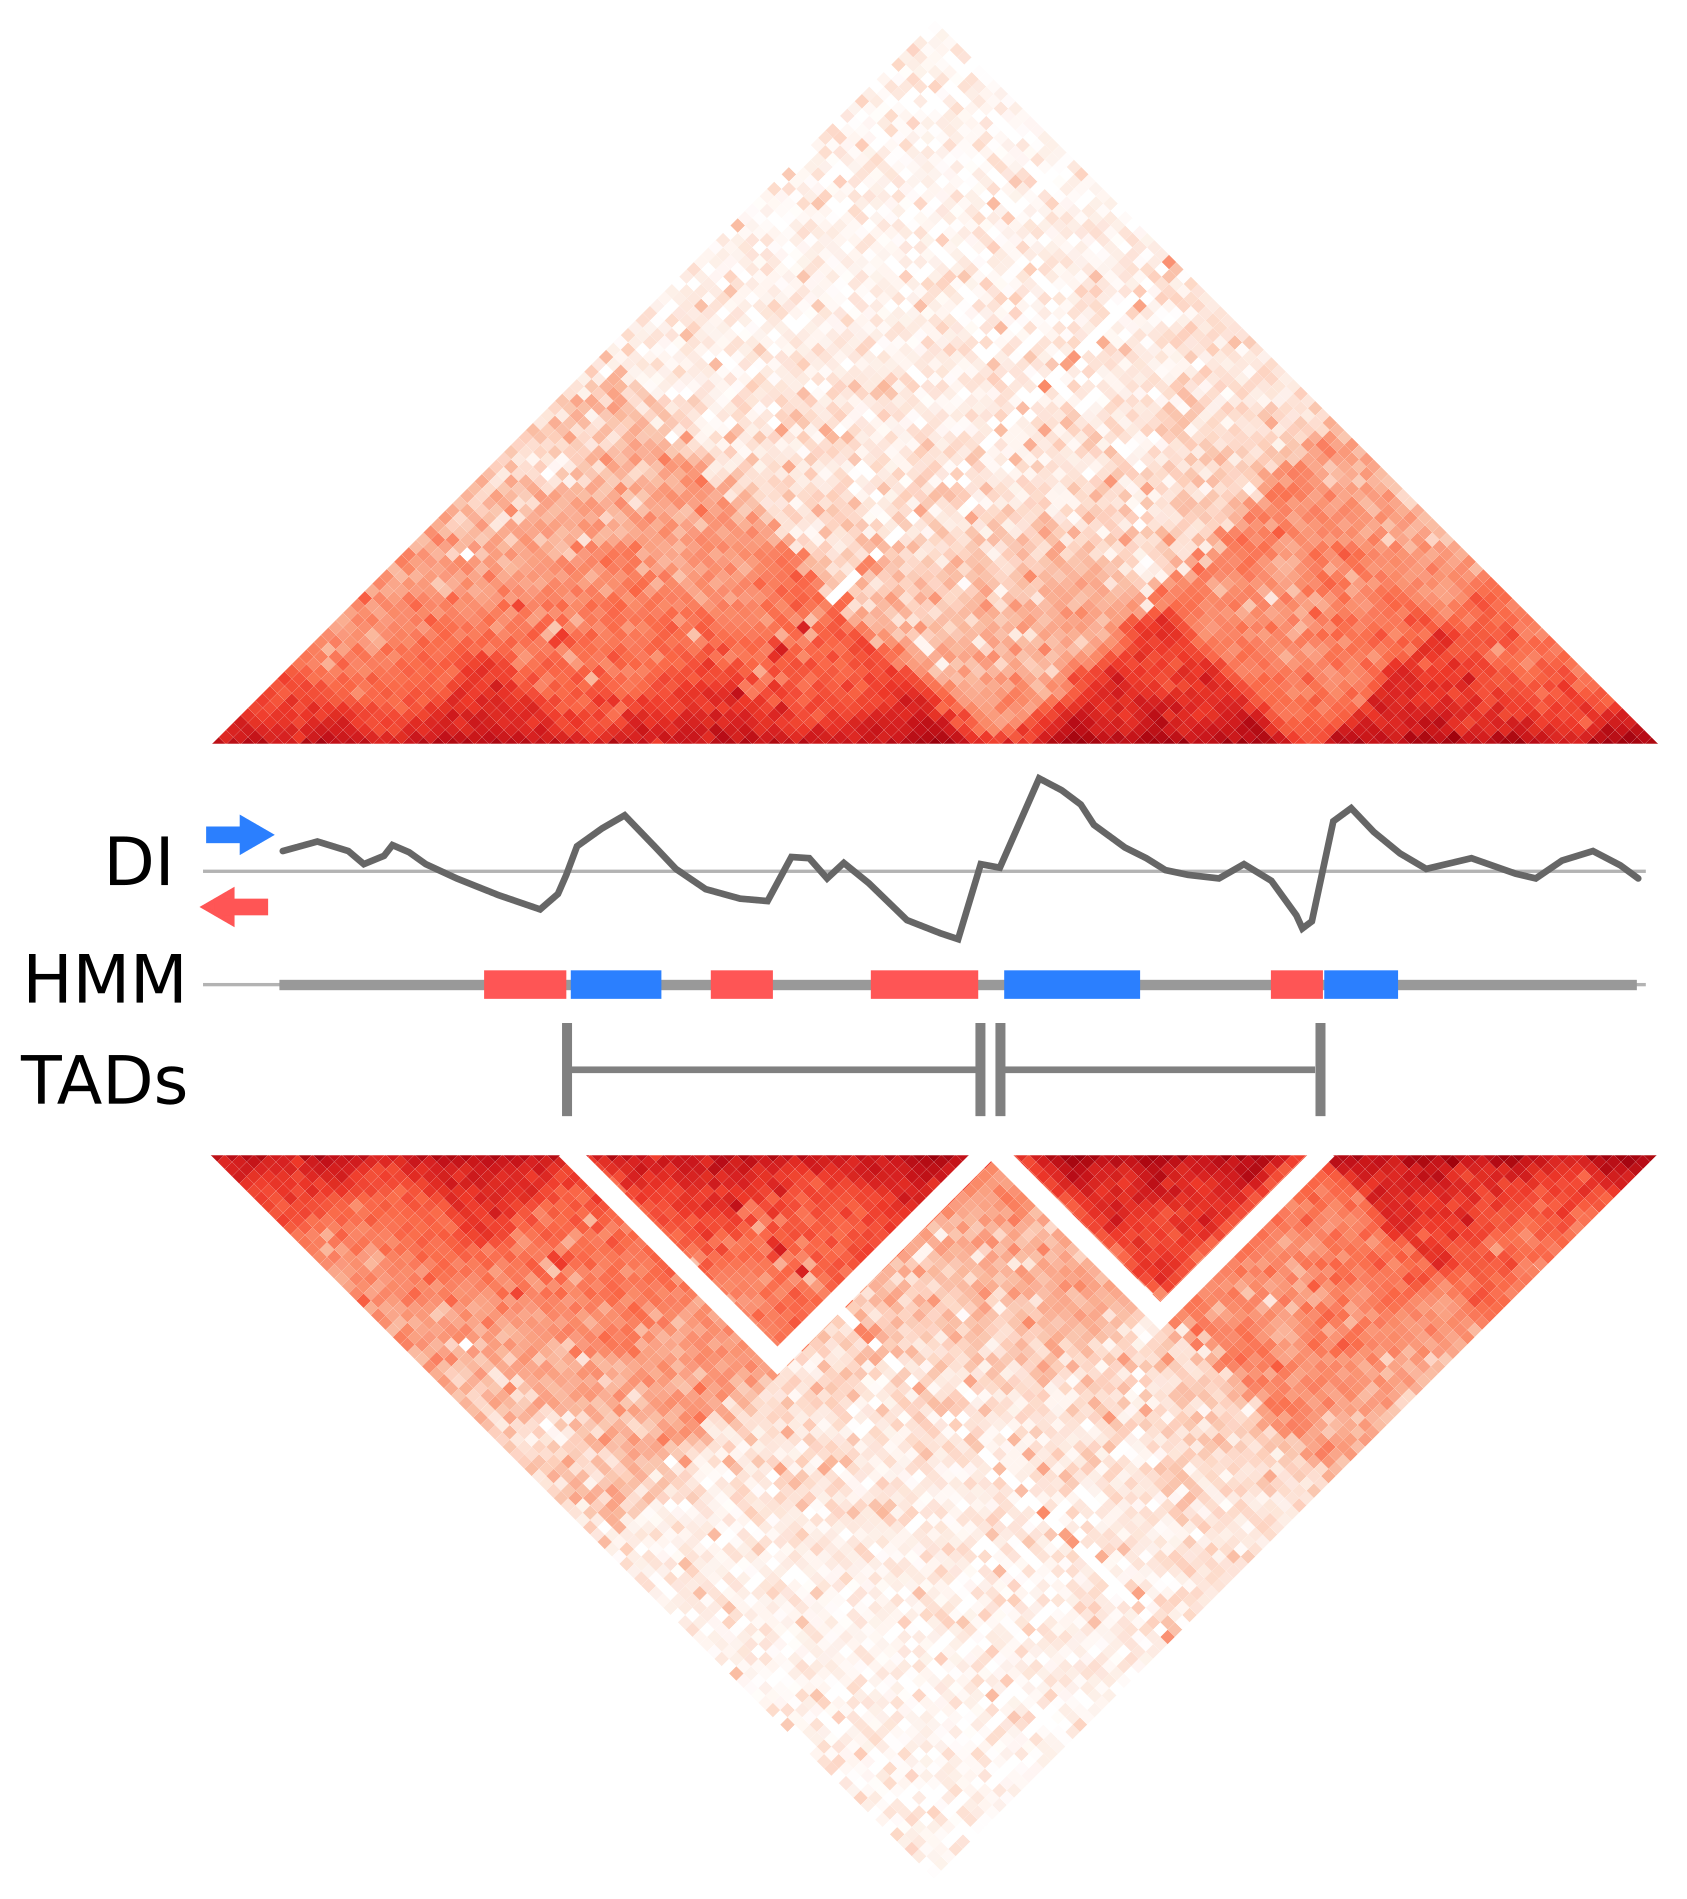
\includegraphics[width=2.5in]{figs/di_example.png}
\captionsetup{width=\textwidth}
\caption[Dixon \emph{et al.} pipeline for calling topological associating domains (TADs).]{ {\bf Dixon \emph{et al.} pipeline for calling topological associating domains (TADs).} First a directionality index (DI) is calculated for each bin based on the ratio of upstream:downstream contacts. Secondly a Hidden Markov Model (HMM) is used to infer the most likely state sequence that emitted the DI variable. Finally a simple rule is applied whereby a run of high-confidence upstream-biased state calls marks the end of a domain. New domains begin with any subsequent downstream-biased state. Gaps between TAD calls can be observed, and as labelled border regions up to a size threshold of 400 kb, whereafter those regions are unclassified.\cite{Dixon2012}
}\label{fig:dicalc}
\end{center}
\end{figure} 

% Function of TADs, regulons, hormone treatment, differentiation etc.
% Sexton2015 review
Since then, several studies have investigated the functional implications of TADs. A simple biological explanation is that TADs---by definition---delimit functional contacts, such as those between enhancers and promoters, and so could inhibit spurious contacts with other nearby genetic elements.\cite{Fraser2015, Sexton2015} Hormonal treatment of human breast cancer cells reported coordinated expression responses within TADs, suggesting they function as domains of transcriptional co-regulation called "regulons".\cite{LeDily2014} However the size of TADs means they often span multiple genes, commonly with unrelated functions, so it seems unlikely they can function as regulons in the general case.\cite{Pombo2015}

\subsection{Other proposed structures}

\citet{Filippova2014} developed a tuneable algorithm which identifies "alternative topological domains". The authors use dynamic programming to search for an optimal set of non-overlapping boundary pairs that maximise intra-domain contacts. The algorithm includes a length scaling factor ($\gamma$) which is used to penalise domain size; by varying $\gamma$ the authors define a subset of "multiscale domains" of heightened persistence across resolutions.\cite{Filippova2014} These multiscale domains were found to be smaller, on average, than those previously reported by \citet{Dixon2012}, despite be applied to the same Hi-C experimental data (mean size: 200 kb as opposed to $\approx 1$ Mb). However the domains of \citet{Filippova2014} show increased intra-domain contacts and stronger boundary enrichments relative to previously-described TADs, indicating this algorithm may generate a more accurate representation of topological domains in mammalian genome organisation. Intriguingly, this study also reports quantitative evidence for hierarchical genome organisation, finding that those domains called at large $\gamma$ will then combine into larger meta-domains as the $\gamma$ penalty decreases.

A study of \emph{Drosophila} embryonic chromosomes found a similarly hierarchical organisation of physical domains, and also was able to relate these to ``epigenomics domains" showing specific sets of enrichment signatures representing active, null, polycomb-associated and telomeric regions.\cite{Sexton2012} 

Recent high-resolution studies have been able to resolve ever-smaller levels of sub-structure. Rao \emph{et al.}\cite{Rao2014} refined the concept of chromosome compartments to "sub-compartments", dividing simple A/B divisions into a total of 5 subtypes. The authors were also able to identify "contact domains" of median size 185 kb, many of which were associated with identifiable individual looping events (Section \ref{intro:loops}).\cite{Rao2014} This domain size is close to those of \citet{Filippova2014} (described above) and the authors here suggest that previously-observed large TADs may be the result of insufficient sequencing; that is, not all boundaries could be detected using 40 kb binned contact maps thus multiple contact domains were unintentionally combined into large domains.

\begin{figure}
\begin{center}
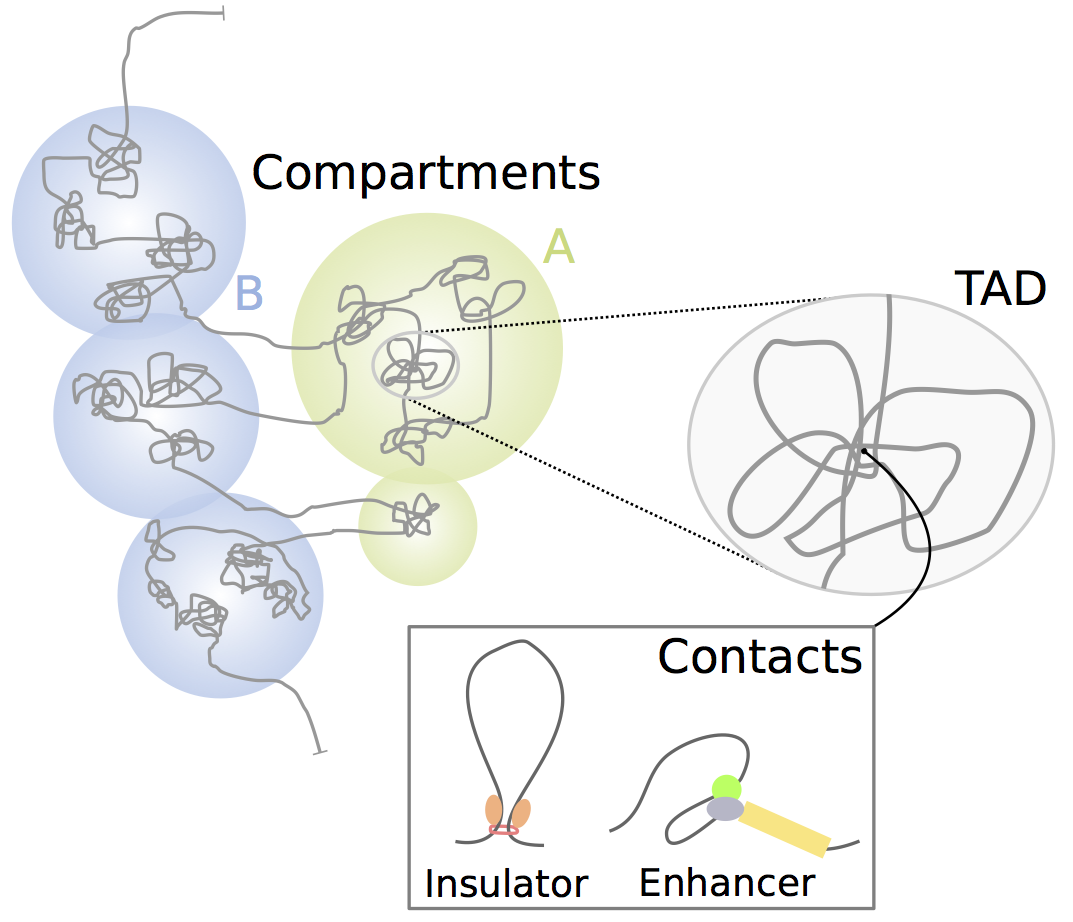
\includegraphics[width=4in]{figs/genome_org.png}
\captionsetup{width=\textwidth}
\caption[Levels of higher order chromatin organisation.]{ {\bf Levels of higher order chromatin organisation. } 
  Cartoon showing how functional contacts, such as loops between bound CTCF insulators (Section \ref{intro:loops}), occur within TADs (Section \ref{intro:tads}) which in turn are found within A or B compartments (Section \ref{sec:compartments}).
}\label{fig:genomeorg}
\end{center}
\end{figure} 

\section{Models of chromatin folding}

Theoretical mechanistic models of chromatin folding such as the
``strings and binders switch'' model\cite{Barbieri2012} and the ``fractal
globule'' model\cite{Lieberman2009, Mirny2011, Grosberg1988a} have both produced simulated data
that reflects empirical C-method observations and potentially describe the polymer
dynamics of chromatin folding.

\begin{figure}
\begin{center}

\includegraphics[width=5.5in]{figs/fractals.pdf}
\captionsetup{width=\textwidth}
\caption[ Comparison of theoretical models of chromatin folding. ]{ {\bf Comparison of theoretical models of chromatin folding. } 
 Two theoretical models of chromatin folding are shown simulated along a 2D polymer, coloured from start to finish as blue--green--red. An equilibrium globule is represented by a Hamiltonian path through a grid network (\emph{left}) and is compared to a Fractal Globule, here represented by a Hilbert curve (\emph{right}).
}\label{fig:fractals}
\end{center}
\end{figure} 

\subsection{Fractal globule}
Lieberman Aiden \emph{ et al.}\cite{Lieberman2009} tested a number of theoretical models of genome folding to see which best explained the observed power-law scaling between distance and observed contact frequency ($\textrm{IF} =  \frac{1}{dist^{-\alpha}}$ where $\alpha \approx 1.08$).  The authors sought to distinguish two previously-described models of genome organisation: the "fractal globule" and "equilibrium globule" (Fig. \ref{fig:fractals}). The study found that a theoretical fractal globule, embodying scale-independent self-similar aggregate folding, better fit the observed data than an equilibrium globule null model where simulated polymer folding was allowed to proceed unchecked.

% cartoon of fractal globule ?
% Dekker2013 has details on these, e.g. vs. equilibrium

The fractal globule model was noted for its appealing functional properties. Under this model, for example, the polymer folds are knot-free hence could facilitate local dynamics of repression and activation without wider disruption. Despite this appeal, the authors were careful to state that while their simulations show good agreement with observed data, this does not preclude other organisational models from having similar or greater explanatory power.\cite{Lieberman2009}

\subsection{Strings and binders switch}\label{intro:sbs}

Subsequent modelling techniques integrated known biological phenomena as well as polymer models. This formed the basis of Barbieri \emph{et al.}'s\cite{Barbieri2012} ``strings and binders switch" (SBS) model, where the authors simulated polymer folding in the presence of DNA binding factors, such as the known genome organiser CTCF (Section \ref{intro:loops}). This organisational model was developed in an attempt to consolidate global Hi-C measures of contact scaling with C-based experiments on smaller regions and FISH studies, which found a range of scaling parameters. The authors also explore the different values of $\alpha$ between cell lines and even chromosomes, and find that their mechanistic model can explain each case using variable concentrations of binders which causes phase-switching between open and compacted chromatin, with fractal globule existing at the phase transition boundary.

This model offers broad explanatory power for a range of observed power law coefficients ($\alpha$) and from simple underpinnings, but critics point out that simulations were performed on a polymer composed of just 512 monomers so may not be broadly applicable.\cite{Dekker2013}

\subsection{Looping and CTCF}\label{intro:loops}

Examples have long been known of specific enhancer elements that are brought into close proximity with the promoter(s) they are regulating; under this model, these contacts form a "loop" structure between two potentially distal loci\cite{Kadauke2009a, Sexton2009} (Fig. \ref{fig:genomeorg}). A model region, the $\beta$-globin locus and its locus control region (LCR) located 40-80 kb away,\cite{Dekker2013} has been studied since the early 1980s,\cite{Banerji1981, Engel2000, Blackwood1998, Tolhuis2002} and is an interesting example of a well-characterised looping. Current knowledge suggests the $\beta$-globin forms loops with the multiple distal \emph{cis}-enhancer elements which make up the LCR, together forming an active chromatin hub (ACH).\cite{VandeCorput2012a} Within such a hub, regulatory signals could be efficiently integrated to dictate the overall activity of the target locus.\cite{DeWit2012, Pombo2015} It is now thought that the majority of active promoters are engaged with multiple, often cell type specific, regulatory looping events.\cite{Sanyal2012, Jin2013}

A notable component of many long-range looping events is the CCCTC-binding transcription factor (CTCF),\cite{Ong2014, Phillips2009} already mentioned as a component of TAD boundaries (Section \ref{intro:tads}) and as a proposed looping factor in the SBS model (Section \ref{intro:sbs}). CTCF is strongly conserved in higher eukaryotes,\cite{Filippova1996a} ubiquitously expressed and embryonic lethal, but it is not tied to a single biological function --- instead CTCF has been described as a "multivalent factor",\cite{Phillips2009} capable of regulating transcription, imprinting, dosage-compensation and acting as an insulator. 

In the context of genome organisation, CTCF is of interest for its role of anchoring interactions between loci, forming loops. Experimental evidence has shown that interactions between CTCF sites stabilises the aforementioned loops linking the $\beta$-globin locus with its distal LCR.\cite{Splinter2006} This looping role, potentially undertaken in combination with other architectural proteins such as Mediator and cohesion,\cite{Phillips-Cremins2013, Sexton2009} can explain its previously-identified insulator behaviour: CTCF can block the spread of heterochromatin and contacts between enhancers and promoter through topological constraints by forming loops.\cite{Phillips2009} It must be said, however, that the functional significance of CTCF-mediated loops, and indeed the role of CTCF in even well-studied systems, remains only partially understood.\cite{Gomez-Diaz2014}

% bring back around to Rao2014 via CTCF
A recent Hi-C paper, that of \citet{Rao2014}, again brought CTCF and looping to the fore of chromatin conformation research. This study identified around $10,000$ individual looping events in the human genome, almost all linking loci over distances of less than 2 Mb, and around $30\%$ connecting predicted enhancer and promoter chromatin states. \citet{Rao2014} also found a 6-fold overall increase in expression when comparing those promoters participating in a looping event with those not. Furthermore, $86\%$ of these loops involved CTCF bound regions, with roughly the same proportion involving cohesion subunits RAD21 and SMC3. The authors thus proposes that a CTCF-binding motif formed the "anchor" for this transitive complex of architectural proteins.\cite{Rao2014} A majority of these loops ($65\%$) also demarcated a topological domain, and at much higher resolution than previously observed (Section \ref{intro:tads}). Another striking finding of this research was that CTCF loops almost always occur in between bound motifs with a convergent orientation,\cite{Rao2014} though questions remain over why this should be the case, especially when considering the interactions of a flexible polymer in 3-D solution.\cite{Nichols2015}

% recently partially addressed with http://www.sciencedirect.com/science/article/pii/S0092867415009691 + Guo et al. (2015) in Cell

While the evidence linking CTCF and genome architecture is substantial, it should be noted that from a global perspective as few as $15\%$ of all CTCF ChIP-seq peaks were found to occur at TAD boundaries in human and mouse cells\cite{Dixon2012} and similarly around $25\%$ if TAD borders had no observable CTCF binding.\cite{Sexton2015} These facts indicate that CTCF alone is neither necessary nor sufficient for the formation of higher order chromatin structures such as TADs. Indeed, the degree of insulation at a given genomic site was recently reported to correlate with the degree of co-binding of a range of architectural proteins including not only CTCF but cohesin, condensin and the transcription complex TFIIIC, among others.\cite{VanBortle2014}

%\subsection{Cell cycle changes}
%
%Chromosome structure has been assayed both through mitosis\cite{Naumova2013} and studies have also focused on the edge-case of chromatin structures on X-chromosomes.\cite{Crane2015}

\section{Criticisms of C-methods}

C-methods are a relatively new and developing set of assays, especially compared to long-standing microscopy techniques which have for decades been used to visualise chromosome conformation. In this section, we discuss some of the limitations and issues with applying or interpreting the results of C-methods.

\subsection{Cell populations}
% cell populations
As previously mentioned (Section \ref{sec:hicvar}), the Hi-C assay typically takes place in a cell population (though proof-of-concept single-cell experiments have been reported\cite{Nagano2013}). An obvious consideration, then, is that all interaction counts reflect the average over a large number of cells, often including unsynchronised populations at different stages of the cell cycle.\cite{Fraser2015} Given evidence that, while the interphase chromosomes exhibit cell-to-cell variability, the mitotic state is much more static,\cite{Naumova2013, Dekker2014} one might expect even a small proportion of dividing cells to add a detectable bias to averaged genome-wide contact maps.

\subsection{Ploidy}
A more esoteric consideration with C-methods data is that organisms under study are typically diploid, while maps of chromosome organisation are commonly collapsed onto a haploid pseudo-genome. Haplotype conformation can be delineated from C-methods data a variety of ways, such as using haploid cell lines (e.g. \citenum{Rao2014}) or via detectable sequence differences using either deep sequencing or a targeted area (e.g. \citenum{Splinter2011}). An altogether different and inventive solution is to use the inherent proximity-ligation information produced by C-methods to discriminate haplotypes,\cite{Selvaraj2013a} an idea since extended to deconvolution problems in metagenomics.\cite{Burton2014, Beitel2014}

% resolution
\subsection{Resolution}
The resolution of a Hi-C experiment has a hard-limit imposed by the choice of restriction enzyme. For example, the commonly-used HindIII enzyme is a six-cutter that recognises the motif AAGCTT and cuts approximately every 4 kb, on average.\cite{DeWit2012} This results in on the order of $10$ million restriction fragments with a total pairwise interaction space of $10^{12}$.\cite{Lajoie2014} The depth of sequencing required to cover this interaction space is cost-prohibitive, so in practice analysis takes place with data aggregated into bins of either fixed length or fixed number of restriction fragments. 

More recent studies have switched to a four-cutter restriction enzyme, for example MboI,\cite{Rao2014} which increases this upper-bound on resolution to the order of hundreds of basepairs (e.g. theoretical mean fragment size of $422$ bp in mouse\cite{Sahlen2015}), but again ultra deep-sequencing is required to realise such resolutions during analysis. A downside of using more frequent restriction enzymes is the potential side-effect of promoting more non-specific ligations by increasing the concentration of fragments in solution.\cite{Rao2014} 

Realistically and in most instances, an experimental design may either target high-resolution interactions through targeted 4C or 5C, or low-resolution genome-wide interactions --- but not both.

\subsection{Biological interpretation}
% For 
% in Lieberman: s^{1/3}  == scaling observed in 3D FISH (500 kb < 2 Mb)
A key consideration with C-methods is that, when accurately stated, the assays are measuring ``the frequency at which sequences are ligated together by formaldehyde cross-linking",\cite{Williamson2014} which is then assumed to be a proxy for physical distance within the nucleus. This is a marked difference from aforementioned FISH methods, where the physical distance is observed directly, albeit through the addition of non-native probes. So strong is this assumption, that methods have been developed that use a known FISH distance to then calibrate genome-wide Hi-C distances,\cite{Shavit2014} however it need not be the case that population-level interaction frequencies capture physical distance.\cite{Lajoie2014} Consider, for example, a tight enhancer--promoter interaction occurring in $50\%$ of cells, but not at all in the other half. In this scenario, the two loci would have an intermediate interaction frequency overall, which is then converted to a distance measure that reflects the realities of neither cell sub-population. For similar reasons, the transience of an interaction cannot be directly inferred from its interaction frequencies: a weak interaction frequency may be the result of either the same fleeting contact in many cells, or stable contacts in only a subset of cells.\cite{Lajoie2014}

%yet it remains unclear to what extent these two methods are compatible.

%Incidental contacts
When interpreting C-methods data it should also be kept in mind that even verifiable contacts are by no-means functional. To elaborate, C-methods may find two regions to be strongly co-localised, but an understanding of the region may explain their co-localisation to be caused by mutual interaction with a nuclear lamina or nucleolus, for example, rather than any specific functional relationship between the two loci.\cite{Dekker2013} In addition, a functional enhancer--promoter interaction will necessarily constrain the contacts of other nearby regions, potentially causing highly-reproducible "bystander interactions"\cite{Dekker2013} that are nevertheless uninteresting from a functional perspective. 

\subsection{Other considerations}
An additional and separate issue identified with C-methods, specifically 3C in this instance, emerges from reports that the observed ligation frequency is as low as $1\%$ of expected values in a model system,\cite{Gavrilov2013} potentially magnifying the relative influence of noise and artefacts.

% something about polymer folding, unavoidable contacts between nearby regions? Refs in Dekker2013: http://www.nature.com/nrg/journal/v14/n6/full/nrg3454.html#ref24


\section{Machine learning in genomics}\label{intro:ml}

Machine learning offers a powerful framework for understanding complex datasets, such as those produced in large-scale genomics studies. Problems in the field such as gene prediction and inferring regulatory networks can be approached by employing a learning algorithm, either in a supervised way based on a known truth set, or through unsupervised methods aimed at pattern detection or clustering (for reviews see \citenum{Jordan2015, Libbrecht2015}). If a successful predictive model can be built, it can then be dissected to explore statistical rules which may impart novel biological insight. As a toy example, learning a highly-accurate model of enhancer prediction could itself identify novel epigenetic marks indicative of enhancers, generating testable hypotheses about how enhancers are activated.

In this section, we introduce recent and high-profile machine learning applications in the context of the ENCODE consortium, and give examples of how their vast datasets have empowered research groups worldwide to tackle complex biological questions through a variety of machine learning approaches. We then discuss research broadly aligned with the aims of this thesis, those attempting to advance an understanding higher order chromatin structure through machine learning and related techniques.

\subsection{ENCODE}\label{intro:encode}

The Encyclopaedia of DNA Elements (ENCODE) is a consortium project started over a decade ago with the ambitious aim of comprehensively cataloguing all functional elements in the human genome.\cite{Feingold2004, Qu2013, Dunham2012} This project involves huge amounts of data production from a diverse array of experimental methods, such as: ChIP-seq, DNase-seq, RNA-seq, CAGE, DNase-seq and ChiA-PET.\cite{Myers2011} Importantly these methods were applied to a range of human cell types, including many well-studied immortalised cell lines as well as primary cells and tissues, and according to standardised experimental methods\cite{Landt2012} coupled with statistical quality control\cite{Dunham2012, Boyle2014, Marinov2013} to ensure data is comparable between different data produces and of consistently-high accuracy. Despite ENCODE's human-focus, there also exists spin-off projects aimed at building similar genomics resources for mouse\cite{Yue2014} and, more recently, \emph{Drosophila} and \emph{C. elegans}.\cite{Ho2014} Together these data sources offer an unparalleled resource for comparative and within-species genomics research, and as such have been used in at least 1200 publications to date.\cite{encodenews}

Data generated by ENCODE consortium members has a proven utility in genomics research. Notably two ENCODE-associated groups have released models which classify the human genome into discrete "chromatin states", such as actively transcribed regions or gene promoters. The first, named \texttt{SegWay}, trained a dynamic Bayesian network on  31 ENCODE-generated input variables and called an unsupervised 25-state genome segmentation in the ENCODE pilot region.\cite{Hoffman2012} Independently another chromatin state predictor named \texttt{ChromHMM} was developed.\cite{Ernst2011, Ernst2012} As the name suggests, this approach instead used multivariate Hidden Markov Models (HHMs) and has the capability to learn a single generative model over multiple cell types. Original runs of the model called 51 chromatin states using over 40 input features,\cite{Ernst2010a} but more recently these two methods were combined to call a consensus set of just 7 chromatin states.\cite{Hoffman2013} Since their publication, a study was able to experimentally validate many of these state predictions.\cite{Kwasnieski2014} This discretisation of the chromatin landscape greatly helps interpretability, at the cost of simplifying the complex underlying data series, and is used for this reason later in this work (Section \ref{sec:chromstateenrich}). 

More broadly, ENCODE data has been used by external researchers to generate input variables for machine learning-based predictive models which describe transcriptional output,\cite{Cheng2011} gene regulation,\cite{Althammer2012} cell cycle-associated genes \cite{Cheng2013} and enhancer identification\cite{Rajagopal2013} to name but a few. One such study in particular, that of \citet{Dong2012}, is reproduced and further analysed in this work (Section \ref{sec:reprodong}) and is used as a template for our own machine learning framework applied in the context of higher order chromatin structure (Chapter \ref{chap:modelling}). We also make use of ENCODE data in other chapters (e.g. Chapter \ref{chap:boundaries}) due to its comprehensive coverage of model human cell types and stringent data production guidelines referenced above.

\subsection{Related work}
% Machine learning + higher order chromatin structure.
In this thesis we will be applying machine learning and other forms of statistical analysis the gain a greater understanding of the biological underpinnings of higher order chromatin conformation (introduced in Section \ref{intro:genomeorg}). We shall now consider existing and overlapping works, some of which were published after or during the time that the research presented herein was performed.

% predicting replication domains

% Sexton predicting TAD boundaries

% Emily regression models of variable regions ?

% predicting Hi-C compartments ?

\section{Aims}

In the broadest terms, the aims of this work are to investigate the relationship between structure and function of the genome. In particular, we aim to answer the following questions: 
\begin{enumerate}
\item How does higher order chromatin structure compare across cell types?
\item Can we predict higher order chromatin structure from locus-level features?
\item How do the characteristics of boundaries remarking higher order domains vary between cell types and domain classes?
\end{enumerate}

In an attempt to address these questions, we will bring together the huge volumes of data generated by the ENCODE consortium (Section \ref{intro:encode}) and employ machine learning techniques and other statistical analysis to explore how these locus-level features relate to higher order chromatin structure. 

\ifstandalone
\begin{small}
\bibliography{/Users/benmoore/Documents/library,/Users/benmoore/Documents/customrefs}
\end{small}
\fi

\end{document}


% ---------- Methods ---------- %
\documentclass[a4paper,11pt,oneside]{book}

% packages 
\usepackage{arsclassica}    % fancy layout
\usepackage[english]{babel}\addto{\captionsenglish}{\renewcommand{\bibname}{References}}
\usepackage{caption}         % figure captions
\usepackage[square,numbers,super,sort&compress]{natbib}  % bibliography style
\usepackage[cc]{titlepic}    % enable logo on title page
\usepackage{graphicx}       % logo related

\usepackage{bm} % bold math
\usepackage{amsmath} % underset
\usepackage{hyperref} % urls
\usepackage[]{algorithm2e}
\usepackage{array}
\usepackage{booktabs}

% Margins for pretty version ::
%\usepackage[pass]{geometry}
% Margins for university regulations ::
\usepackage[top=2cm, bottom=4cm, left=4cm, right=2.5cm]{geometry}
\usepackage{setspace}
\onehalfspacing

% don't hang captions
\captionsetup{format=plain}

\newcolumntype{L}{>{\centering\arraybackslash}m{4cm}}
\definecolor{light-gray}{gray}{0.95}

\usepackage{standalone}
\standalonetrue 

% bibliography
\bibliographystyle{../thesis}

% title setup
\title{ \vspace{3in} Unravelling higher order genome organisation {\small [working
    title]} \\ \vspace{2em} {\large {\bf Methods section}} }
\author{Benjamin L. Moore}
\titlepic{\vspace{2.2in} 
\includegraphics[width=\textwidth]{/Users/benmoore/hvl/1yrReport/figs/igmm.png}}

\begin{document}

%\maketitle

\chapter{Methods}

\section{Hi-C data}\label{methods:hic}

\subsection{Mapping}\label{methods:mapping}

Raw Hi-C reads were downloaded from published datasets (Table \ref{hictable}) through
the Gene Expression Omnibus (GEO)\citep{Barrett2013} or the Short Read Archive (SRA)\citep{Leinonen2011a} with identifiers:
GSE35156 (H1 hESC), GSE18199 (K562) and SRX030113 (GM12878). These
paired reads were mapped independently to a reference genome: hg19/GRCh37 for human data, and mm10/GRCm38 for mouse. 

\begin{table}
\centering
\caption[Public Hi-C data used in this work.]{ {\bf Public Hi-C data used in this work.} }
\label{hictable}
\begin{tabular}{lllr}
{\bf Cell line} & {\bf Total reads} & {\bf Accession} & {\bf Citation}\\
\hline
Gm12878 & 31$\times10^{6}$ & \href{http://www.ncbi.nlm.nih.gov/sra/SRX030113[accn]}{SRX030113} & \citenum{Kalhor2012} \\
H1 hESC & 331$\times10^{6}$ & \href{http://www.ncbi.nlm.nih.gov/geo/query/acc.cgi?acc=GSE35156}{GSE35156} &\citenum{Dixon2012} \\
K562 & 36$\times10^{6}$ &  \href{http://www.ncbi.nlm.nih.gov/geo/query/acc.cgi?acc=GSE18199}{GSE18199}  & \citenum{Lieberman2009} \\
\hline
Cortex & 373$\times10^{6}$ & \href{http://www.ncbi.nlm.nih.gov/geo/query/acc.cgi?acc=GSE35156}{GSE35156}& \citenum{Dixon2012} \\
mESC & 476$\times10^{6}$ & \href{http://www.ncbi.nlm.nih.gov/geo/query/acc.cgi?acc=GSE35156}{GSE35156}&\citenum{Dixon2012} \\
\hline
IMR90 & 355$\times10^{6}$ &\href{http://www.ncbi.nlm.nih.gov/geo/query/acc.cgi?acc=GSE35156}{GSE35156} &\citenum{Dixon2012} 
\end{tabular}
\end{table}

Mapping was performed using the \texttt{hiclib} software
package\citep{Imakaev2012} and \texttt{bowtie2}\citep{Langmead2012} with
the \texttt{-{}-very-sensitive} flag. An iterative mapping approach was used to maximise the number of aligning fragments.\cite{Imakaev2012} Each fragment end was aligned first using short terminal sub-sequences. Those unmapped or with ambiguous mapping were then taken forward into the next iteration and extended until the entire fragment end had been aligned. Those remaining pairs with one or more unmapped ends were discarded.

This approach is designed to maximise uniquely-alignable fragment ends, while avoiding mismappings caused by crossing the fragment junction.\cite{Lajoie2014} 

\subsection{Filtering}\label{methods:filtering}

After mapping, interactions are first aggregated into restriction fragments then by regular binning of various resolutions (particularly 40 kb, 100 kb and 1 Mb). Several filters were applied at this stage, with the following cases removed:\cite{Imakaev2012, Lajoie2014} 
\begin{itemize}
\item Reads directly adjacent to a restriction enzyme site (within 5 bp)
\item Identical read pairs (presumed PCR duplicates)
\item Very large restriction fragments ($>100$ kb) which are likely from a repetitive or poorly-assembled region
\item Extremely over-represented fragments (top $.05\%$) which may throw-off eigenvector derivation
\end{itemize}

\subsection{Correction}\label{methods:correction}

Iterative correction and eigenvector expansion (ICE) is an approach to normalisation and processing Hi-C data, implemented as software library written in \texttt{python}.\citep{Imakaev2012} The iterative correction algorithm performs matrix balancing with the aim of generating a doubly stochastic matrix from raw interaction counts.\cite{Lajoie2014} That is, such that symmetric matrix $\mathbf{A}$ has both row and columns of equal sum. In practice, this effectively enforces "equal visibility" of each fragment, correcting for previously-described biases in interaction recovery such as GC-content and fragment length\cite{Yaffe2011} but without explicitly modelling these latent variables. This procedure is thus converting actual interaction counts into normalised interaction frequencies (IF), and to relative rather than absolute quantities. Scaling of IFs permits comparison of Hi-C experiments with very different sequencing depths (as is the case in this work, see Table \ref{hictable}). Despite differences in the levels of sequencing, otherwise the experiment methods underlying the produced Hi-C data were similar: the HindIII restriction enzyme was used in each case and the Hi-C protocol was largely unchanged (that is, we did not consider data from Hi-C variants such as TCC\cite{Kalhor2012} and \emph{in-situ} Hi-C\cite{Rao2014}).

\subsection{Eigenvector calculation}\label{sec:eigs}
Additional functionality provided by ICE is the eigenvector expansion of normalised contact maps. Eigenvectors from observed/expected matrices were chosen for consistency with Lieberman Aiden \emph{et al.},\cite{Lieberman2009} as opposed to the related eigenvectors calculated in Imakaev \emph{et al.}\cite{Imakaev2012} from the corrected maps alone. The details of this procedure are described in section \ref{sec:compartments}. Briefly, observed contacts (O) are divided by an expected matrix (E) which is generated by averaging the super- and sub-diagonals of the O matrix. That is, the E matrix gives the expected value of interactions at a given distance.

Importantly, the first two principle components (PCs) were calculated, and that with the highest absolute Spearman correlation with GC content is taken to reflect A/B compartmentalisation. PC eigenvectors were then orientated to positively correlate with GC, ensuring positive values reflected A compartments and negative values B compartments. Another subtlety is the calculation of eigenvectors per chromosome arm as opposed to per chromosome, this prevents issues with some meta- and submetacentric chromosomes where the first principle component indicated chromosome arms.\cite{Lieberman2009, Imakaev2012} Eigenvector expansion was performed on both 1 Mb and 100 kb matrices, below these resolutions results became less stable, and besides it has been shown that eigenvectors at higher resolution --- when they do indeed capture A/B compartmentalisation --- add little, if any, additional information.

\section{ENCODE features}\label{methods:encode}

Genome-wide ChIP-seq datasets for: 22 DNA binding proteins and 10
histone marks were made available by the ENCODE
consortium\citep{Dunham2012, Boyle2014} along with DNase I
hypersensitivity and H2A.z occupancy, for each of the Tier 1 ENCODE cell
lines used in this work: H1 hESC, K562 and GM12878. These data were
pre-processed using MACSv2\citep{Zhang2008} to produce fold-change
relative to input chromatin. GC content was also calculated and used in
the featureset to give 35 total inputs (Table \ref{tab:features}).

\begin{table}[h]
\centering
\caption{ ChIP-seq and other public datasets used in this work. }
\label{tab:features}
\begin{tabular}{L | L | c} \toprule
\multicolumn{1}{m{4cm}}{\centering Histone modifications} &
\multicolumn{1}{m{4cm}}{\centering DNA binding proteins} &
\multicolumn{1}{m{2cm}}{\centering Other} \\
\midrule

% histone modifications
H3K27ac, 
H3K27me3, 
H3K36me3, 
H3K4me1, 
H3K4me2,  
H3K4me3, 
H3K79me2, 
H3K9ac, 
H3K9me3, 
H4K20me1 &

ATF3, CEBPB, CHD1, CHD2, CMYC, CTCF, EGR1, EZH2, GABP, JUND, MAX, MXI1, NRSF, POL2, P300, RAD21, SIX5, SP1, TAF1, TBP, YY1, ZNF143 &

\multicolumn{1}{m{2cm}}{\centering DNase, GC content, H2A.Z }\\

\end{tabular}
\end{table}

\subsection{Clustering input features}

To quantify collinearity of input features, correlation matrices built from genome-wide vectors of input feature measures were build and hierarchicaly clustered. The "significance" of observed clustering was assessed using sub- and super-sampled bootstrapping, with stable clusters deemed significant, as implemented in the \texttt{pvclust} R package.\cite{Suzuki2006a}

\section{Modelling}\label{modelling}

\subsection{Random Forest}\label{sec:rf}

\begin{figure}
\begin{center}
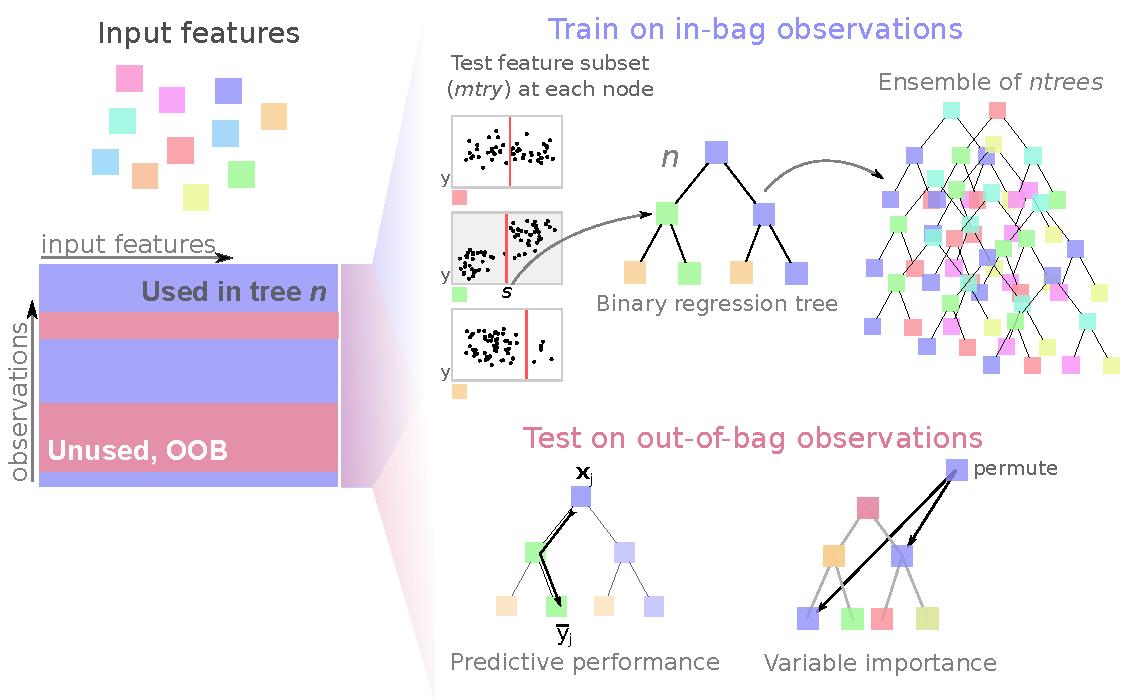
\includegraphics[width=4.5in]{figs/randforests.pdf}
\captionsetup{width=\textwidth}
\caption[Random Forests overview.]{ {\bf Random Forests overview. } 
 Random Forests are an ensemble of bagged, de-correlated classification or regression trees first described by Breiman.\cite{Breiman2001a}
}\label{fig:randforests}
\end{center}
\end{figure} 

Random Forest (RF) regression,\cite{Breiman2001a}  was used
as implemented in the R package \texttt{randomForest}.\cite{Liaw2002}
The RF algorithm (Fig. \ref{fig:randforests}) makes use of a collective of regression trees (size $ntrees$), each built from a
bootstrapped sample of the training set. In growing each tree, a small
number of variables ($mtry$) is tested at each bifurcation node, and that which minimises the
variance in child node subsets is selected at a specific
threshold. Having trained a group of trees, these can then be used as
predictive tools by inputting a vector of features to each tree and
averaging the output leaf node value across the forest. RF regression
was used as it is known to be one of the most powerful regression
methods developed to date,\cite{Svetnik2003, Cutler2007} typically
providing low bias and low variance predictions without the need for
variable selection.\cite{Diaz2006, Dasgupta2012}

Additionally the RF method represents an example of ``algorithmic
modelling''\cite{Breiman2001b} in that it makes no assumptions about the
underlying data model.
Parameters of $mtry = \frac{n}{3}$ (where $n$ is the number of input features) and $ntrees =
200$ were assumed as they are known to be
largely insensitive;\cite{Dasgupta2012, Hastie2001} this was verified
with the dataset used in this work (Fig. \ref{fig:rfparam}). 

\begin{figure}
\begin{center}
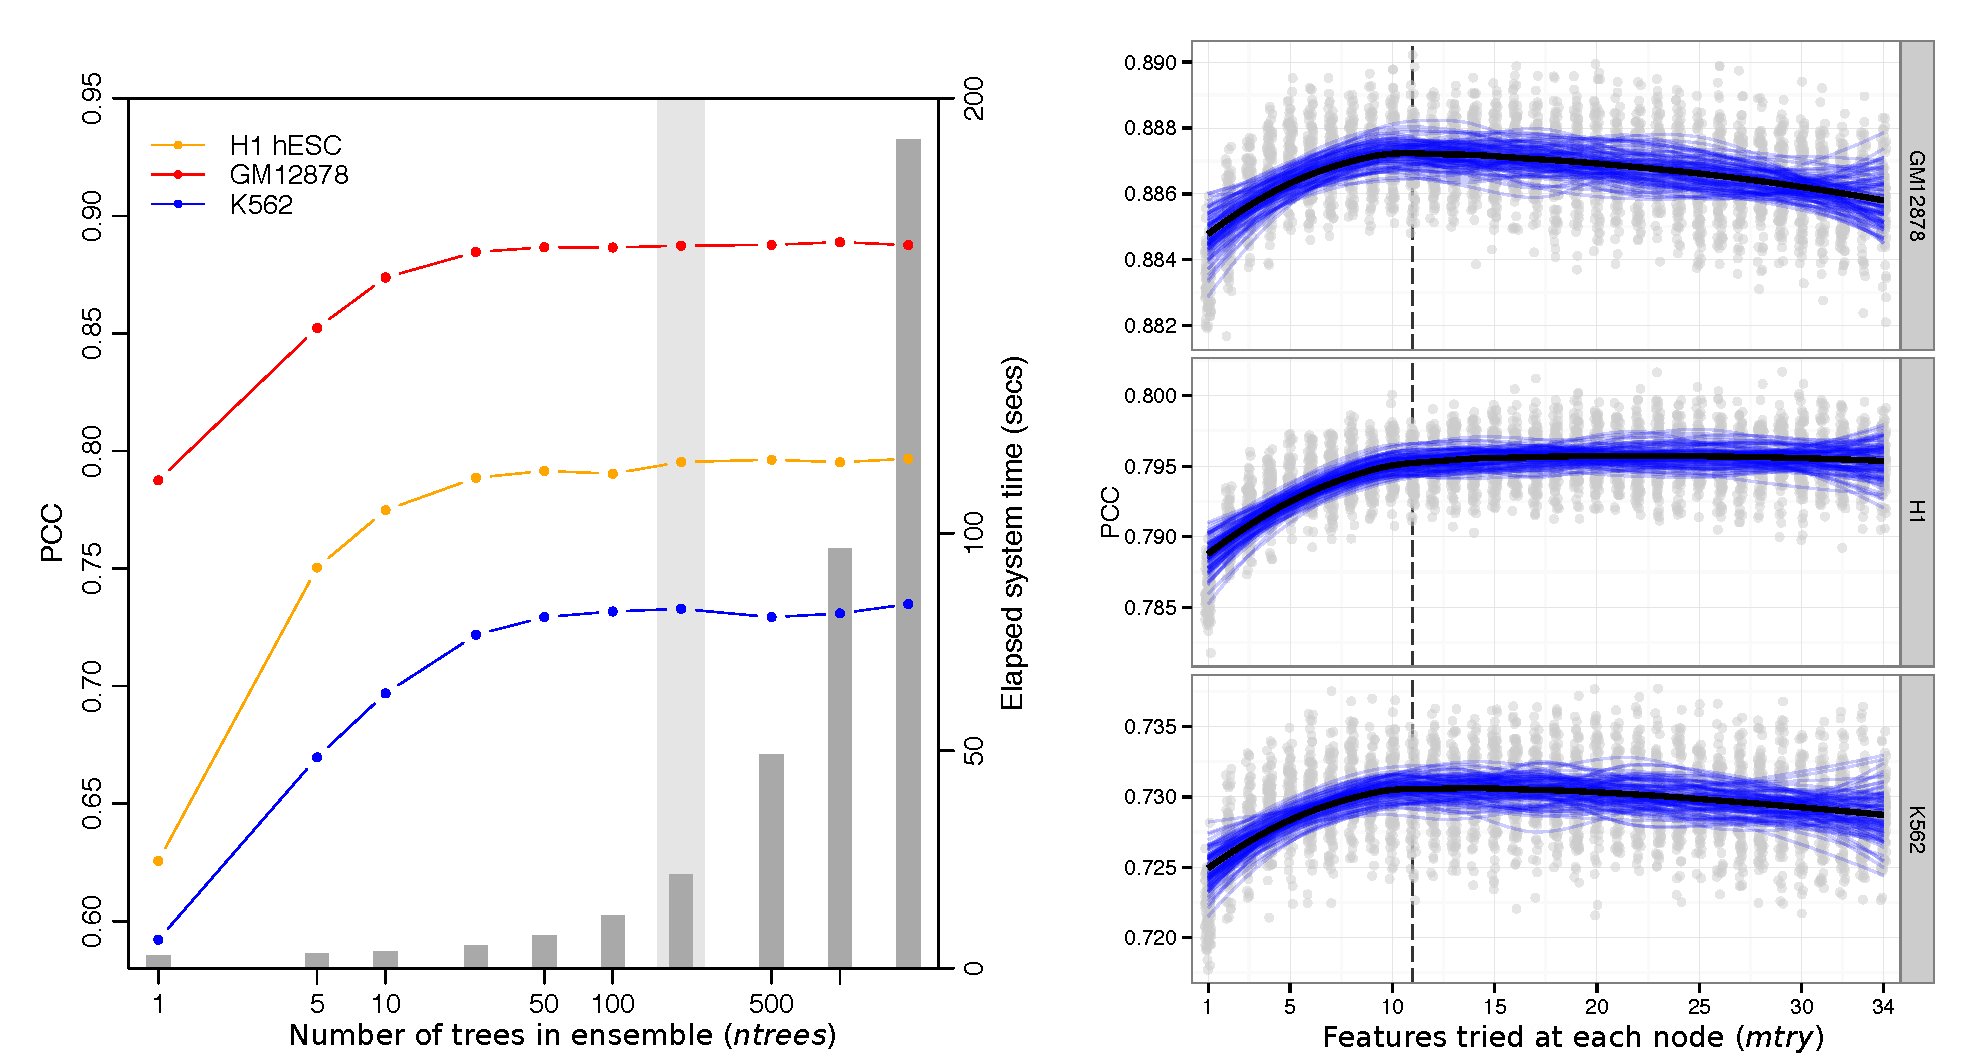
\includegraphics[width=5in]{figs/rfparams.pdf}
\captionsetup{width=\textwidth}
\caption[Random Forest parameters are largely insensitive.]{ {\bf Random Forest parameters are largely insensitive. } 
Two user-facing Random Forest paramters are known to be insensitive over a broad range.\cite{Hastie2001} Optimisations for $ntrees$ (the number of trees in the forests) and $mtry$ (the number of features tested at each node) are shown for three different models, with typical values of 200 trees and $\frac{1}{3}$ of input variables highlighted.
}\label{fig:rfparam}
\end{center}
\end{figure} 

Variable importance within Random Forest regression models was measured
using mean decrease in accuracy in the out-of-bag (OOB) sample. This
represents the average difference (over the forest) between the accuracy
of a tree with permuted and unpermuted versions of a given variable (Fig. \ref{fig:randforests}), in
units of mean squared error (MSE).\citep{Cutler2007, Dasgupta2012}

\subsection{Model performance}\label{sec:modelperf}

The effectiveness of the modelling approach was measured by four
different metrics. Prediction accuracy was assessed by the Pearson
correlation coefficient between the OOB predictions and observed eigenvectors, and the root mean-squared
error (RMSE) of the same data. Classification error, when predictions
where thresholded into $A \geq 0; B < 0$, was also calculated using
accuracy (\% correct classifications or True Positives) and area under
the receiver operating characteristic (AUROC) curve. Together these give
a comprehensive overview of the model performance, both in terms of
regression accuracy of the continuous eigenvector, and in how that same
model could be used to label discrete chromatin compartments.

For cross-application of cell type specific models, a single Random
Forest regression model was learned from all 1 Mb bins for a given cell
type. This was then used to predict all bins from each of the other two
cell types.

To test the sensitivity of the models to resolution, we also applied cell-type specific models learnt at 1 Mb resolution to input features binned at 100 kb. 

\subsection{Other modelling approaches}
 
Linear regression was used as a baseline for comparison with more complicated approaches such as Random Forest. If the same modelling accuracy could be achieved with simple multiple linear regression, this would be a faster and more interpretable modelling framework.

Partial least squares (PLS) regression was also used to model compartment profiles. PLS regression is well-suited to highly correlated inputs, employing a dimensionality reduction step to help address this redundancy, yet lacks the interpretability of a multiple linear regression. Similar to RF, PLS regression is aimed at building highly-predictive models rather than understanding singular relationships between a predictor and independent variable.\cite{Tobias1995} The \texttt{plsdepot} R implementation of PLS regression was used in this work.

%\subsection{Graphical lasso}
%Regularised models made use of the Graphical LASSO\cite{Friedman2008}
%(least absolute shrinkage and selection operator) as a method of
%$L_1$-norm based
%regularisation, implemented via the \texttt{glasso} R package. The
%graphical lasso provides tuneable regularisation which is
%capable of feature selection via minimising regression parameters to
%0. It was chosen in this case due to the multicollinearity of the
%featureset, the algorithm's fast speed of
%execution and the intuitiveness a graphical model
%presents.\cite{Friedman2008} 
%
%More specifically, the graphical lasso regulates the number of 0s in
%the inverse covariance matrix, $\bm{\Theta}=\bm{\Sigma}^{-1}$, also known as the
%precision matrix. Then if element $\theta_{ij}=0$, the variables $X_i$ and $X_j$ can be said to be
%conditionally independent, given the remaining
%variables.\cite{Mazumder2012} The algorithm minimises a negative
%log-likelihood (Eqn. \ref{eq:glasso}\cite{Mazumder2012}) given the tuning parameter $\lambda$, which was tuned
%in this case to leave a small number of variables ($<10$)
%directly dependent on the eigenvector data. \\
%\begin{equation} \label{eq:glasso}
%\underset{\bm{\Theta}\prec\bm{0}}{\mathrm{minimise}}~f(\bm{\Theta}) :=
%-\log\det(\bm{\Theta}) + \mathrm{tr}(\bm{\mathrm{S}\Theta}) + \lambda
%\lVert\bm{\Theta}\rVert_1
%\end{equation}

\section{Variable regions}\label{variable-regions}

\subsection{Stratification by
variability}\label{sec:variable}

Median absolute deviation (MAD) was chosen as a robust measure of the
variability in a given 1 Mb block between the three primary cell types
used in this work: H1, K562 and GM12878. Blocks were ranked by this
measure and split into thirds that represented ``low'' variability (the
third of blocks with the lowest MAD), ``mid'' and ``high'' variability.
Each subgroup was then independently modelled using the
previously-described Random Forest approach.

``Flipped'' regions are those whose compartment state differs in one
cell type relative to the other two. For example, if a 1 Mb bin was
classified as ``open'' in H1 hESC and ``closed'' in both K562 and
GM12878, this is said to be a ``flipped'' compartment (to open).

\subsection{Enhancer enrichment}\label{enhancer-enrichment}
%explanation of combined states: http://rohsdb.cmb.usc.edu/GBshape/cgi-bin/hgTables?db=hg19&hgta_group=regulation&hgta_track=wgEncodeAwgSegmentation&hgta_table=wgEncodeAwgSegmentationCombinedGm12878&hgta_doSchema=describe+table+schema

Chromatin state annotations used in this work were retrieved from the ChromHMM\cite{Ernst2011} and SegWay\cite{Hoffman2012} combined annotations.\cite{Hoffman2013} These represent the consensus from two independent chromatin state prediction algorithms, and ignore regions of apparent disagreement; hence in theory making more robust and conservative predictions than either algorithm independently. Nevertheless, Hoffman \emph{et al.} caution that in areas of disagreement, each algorithm may highlight differing biological phenomena so should also be considered separately.\cite{Hoffman2013}

The set of state predictions from the combined algorithms are:
\begin{enumerate}
\item Predicted transcription start sites (TSS)
\item Promoter flanking regions
\item Transcribed reigons
\item Repressed regions
\item Predicted enhancers
\item Predicted weak enhancer or \emph{cis} regulatory element
\item CTCF-enriched elements
\end{enumerate}

Short, discrete state predictions such as enhancers were
considered ``shared'' if there was an overlapping enhancer annotation in
either of the two other cell types, and labelled as ``tissue-specific''
otherwise. This was repeated for each of the called chromatin states.

\subsection{Gene ontology analysis}

Variable regions (section \ref{sec:variable}) were tested for functional enrichments using Gene Ontology (GO) annotations.\cite{Ashburner2000} The DAVID tool\cite{Huang2008} was used to compare GO terms for genes located in variable compartments with a background set of genes within all annotated compartments.


\section{Boundaries}\label{boundaries}

\subsection{TADs}\label{tads}

TAD boundaries were called using the software provided in
\citet{Dixon2012} using their recommended parameters. For the generation
of boundary profiles, input features were
averaged into 40 kb bins spanning $\pm450$ kb from the boundary bin.

To test for the enrichment or depletion of a chromatin feature over a
given boundary, a two tailed Mann-Whitney test was used to compare the
boundary bin with the ten outermost bins of the window (5 from either
side). The significance level at $\alpha = 0.01$ was then
Bonferonni-adjusted for multiple testing correction, and results with
\emph{p}-values exceeding this threshold were deemed significantly
enriched or depleted at a given boundary.

To compare boundaries between cells, each TAD boundary called in K562 and GM12878 were compared with those called in H1 hESC. For each boundary, the minimum absolute difference to the nearest matching boundary in H1 hESC was recorded, and this was then compared with a null model of an equal number of boundaries randomly-placed along available bins. A Kolmogorov-Smirnov test was then used to compare the empirical cumulative distributions of these distances.

\subsection{Compartments}\label{sec:compartments}

Eigenvectors were calculated as described in section \ref{sec:eigs}. A/B compartmentalisation has previously been called simply from the properly-orientated principle component eigenvector, with positive values representing a bin in an A compartment state, and negative values representing a bin in a B, more repressive state.\cite{Lieberman2009} 

Compartment boundaries were called by first training a two-state hidden
Markov model (HMM) on the compartment eigenvector and then using the
Viterbi algorithm to predict the most likely state sequence that
produced the observed values. Justification for this approach is discussed in Section \ref{sec:compcalls}. 

%HMM states distribution plots

The point at which transitions occurred
between states was taken as a boundary which was then extended $\pm 1.5$~Mb to give a $3$~Mb window in which a boundary was though to occur. Boundary enrichments and alignments were tested in the same manner as TADs (Section \ref{tads}).

\section{MetaTAD analysis}

\subsection{Size selection}\label{sec:metatad}

MetaTADs are a concept discovered by collaborators. Their method for calling such features involve the constrained hierarchical cluttering of neighbouring TADs with the greatest inter-TAD contacts. This results in a tree of increasing metaTAD aggregation. For boundary analysis of metaTADs, again a similar approach was used to that of TADs (section \ref{tads}) but thresholded to within a given range of sizes. MetaTADs below 10 Mb were excluded, as to have no lower bound results in $\frac{2}{3}$ of all TAD boundaries likewise considered MetaTAD boundaries, reducing the power to analyse any differences. 10 Mb was chosen in an attempt to compromise minimising the overlap between TAD and metaTAD boundaries, while also retaining a large enough sample size. An upper bound of 40 Mb was also chosen, as beyond this threshold inter-TAD contacts were found to be no higher than expected by chance. In practice, the tree-like structure means any upper-bound has little impact as a filter: in almost all cases, any boundary in a metaTAD of size $> 40$ Mb will also form metaTADs below this value. Additionally, the hierarchical nature of metaTADs means that some boundaries are present at multiple levels of the tree. Only one case of each boundary position was tested for feature enrichments, and this was performed as with TAD boundaries (Section \ref{tads}).

\subsection{Collaborator datasets}
%CAGE, ctss
Our collaborators in the metaTAD project performed ChIP-seq experiments for PolIII (three variants), H$3$K$27$me$3$, CTCF and DNase-I hypersensitivity. Mapped reads from these experiments were processed using MACSv2\cite{Zhang2008} to give relative signal over background (from an estimated local model), which was then averaged over all boundaries genome wide. 

Cap analysis of gene expression (CAGE) data was produced by the FANTOM consortium.\cite{fantom5, itoh2012a} This method produces sequencing data from the $5`$ end of cDNAs, and can be used to quantify expression activity at precise promoter locations.\cite{Kodzius2006} Here, CAGE was performed at multiple points along a neural-differentiation timecourse and tags were clustered to form CAGE TSS (CTSS) in a manner developed for the FANTOM5 project.\cite{fantom5} To count these CTSS over boundary bins, we simply intersect the annotations and count CTSS per bin using \texttt{bedtools}.\cite{Quinlan2010}

Gene density over metaTAD boundaries was calculated using UCSC \texttt{mm9} gene models.\cite{Karolchik2014} Again simple intersections were taken to count genes over boundaries using \texttt{bedtools}\cite{Quinlan2010} and requiring a minimal overlap fraction of $0.5\%$ of a bin ($250$ bp).

\subsection{LAD coincidence}

To compare metaTAD boundaries with those of LADs, we made use of previously-published Lamin-B1 DamID microarray probe intensities.\citet{Peric-Hupkes2010} For analysis over boundaries, these values were averaged into the same boundary windows as used previously (50 kb bins $\pm450$ kb around boundary, as in Section \ref{tads}). 

Transitions between high and low lamina association were detected by fitting a linear regression model across each series of consecutive boundary bins (i.e. $\textrm{Lamina association}=\beta\cdot\textrm{bin} + c$). Linear models which had an absolute coefficient $|\beta| >.05$ were taken as crossing a LAD transition. This threshold is a heuristic which appears to perform well at conservatively selecting clear transitions. As a method of seriation for the $y$-axis of heatmap figures (e.g. Fig. \ref{fig:mtlamin}), boundaries were divided into those that coincided with a lamin transition and those that did not, and members within each group were then sorted by average intensity. 

To test the significance of the association between boundaries and lamin transitions, we circularly permuted both TAD and metaTAD boundaries on each chromosome 1000 times, and calculated the proportion of boundaries that crossed LAD boundaries using the same linear regression procedure described above. Empirical $p$-values were then calculated as the number of permuted results greater than or equal to the observed value.

\section{Giemsa band comparison}\label{giemsa-band-comparison}

Cytogenic band data and Giemsa stain results were downloaded from the
UCSC genome browser (table \texttt{cytoBandIdeo}). The genomic
co-ordinates are an approximation of cytogenic band data inferred from a
large number of FISH experiments.\citep{Furey2003}

To compare G-band boundaries with our compartment data, we allowed for a
$\pm 500$ kb inaccuracy in G-band boundary. For each G-band boundary,
the minimum absolute distance to any compartment or TAD boundary was
calculated for each cell type. To generate a null model, \ldots

\section{Nuclear positioning}
Previously published data  on chromosome positioning preference within
the nucleus was used to label each chromosome as ``inner'', ``middle''
or ``outer''.\cite{Boyle2001} Chromosomes whose DAPI hybridisation
signals were significantly enriched ($p\leq 2\times10^{-2}$) in the inner nuclear shell, as
defined by Boyle \emph{et al.}\cite{Boyle2001}, made up the ``inner''
group and included chromosomes 1 and 16. Similarly the ``outer'' group
had enriched signals ($p\leq 5\times10^{-3}$) in the outer shell relative to the inner nuclear
shell and included chromosomes 2, 3, 11-13 and 18. The remaining
chromosomes in our filtered dataset, 6, 14 and 15, were assigned to
the ``middle'' group and showed no significant to either inner or
outer nuclear shells ($p \geq 0.1$).\cite{Boyle2001} The significance
of the difference in distribution of eigenvectors in the inner
versus outer shell was determined by a one-sided Kolmogorov-Smirnov (K-S)
test, with the alternative hypothesis that the empirical cumulative
density function of the inner chromosome eigenvectors $F_{inner}$
is greater-than or equal-to $F_{outer}$. This chromosomal positioning data was measured in lymphoblastoid
cells though nuclear architecture is though to be largely conserved
between cell types\cite{Chambers2013, DeWit2013} and even higher primates.\cite{Tanabe2002}

\section{4C analysis}\label{methods:4c}

The experimental protocol used by our collaborators to generate 3C-seq data (also known as 4C) recommends the \texttt{r3Cseq} R package,\cite{Stadhouders2013, Thongjuea2013} part of the bioconductor repository\cite{Gentleman2004, Huber2015} for the R programming environment.\cite{Ihaka1996}

This package functions both to produces normalised interaction frequencies which are comparable between experiments, and to assign statistical significance to any identified contacts, thereby reporting regions that co-localise to a greater degree than expected by their genomic proximity alone.

\subsection{Normalisation}\label{methods:4cnorm}

The normalisation procedure is adapted from a previous method for normalising deepCAGE data between samples.\cite{Balwierz2009} In short, the reverse-cumulative distribution of read counts per restriction fragment is fit to a power-law model; this effectively encodes the \emph{a priori} expectation of exponential decay of the number of contacts as distance increases from the viewpoint. Transformed read counts per million (RPM) can then be retrieved from a standardised reverse cumulative distribution, parametrised with the empirical coefficient, $\alpha = -1.35$.\cite{Thongjuea2013}

This normalisation procedure has the effect of making the output RPM value independent of the original experiment's sequencing depth and, more importantly, acts to reduces the impact of artefacts and errors by enforcing the expected power-law relationship of restriction fragment read counts.

\subsection{Significance estimation}\label{methods:4csignif}

The \texttt{r3Cseq} package\cite{Thongjuea2013} also attempts to assign a measure of significance to observed contact frequencies. This is done through a simple method of background estimation based on observed values. The justification for this non-independent estimate of background signal is that a relatively small proportion of observed contacts are expected to be significantly enriched, thus won't unduly perturb an average signal.\cite{Thongjuea2013} An improved method that avoids this assumption has since been developed where a background model was iteratively fitted, with outlier removal at each revision.\cite{Ay2014}

Here a non-parametric cubic smooth spline is fit to normalised read count data using a heuristic smoothing parameter. This model then provides an expected level of interaction at a given distance from the viewpoint in \emph{cis}. From this, it is simple to calculate a $Z$--score as:

\begin{equation}\label{form:r3cseq}
Z = \frac{(O-E)}{\sigma}
\end{equation}

\noindent Where $\sigma$ is the standard deviation of residuals from the observed ($O$), expected ($E$) difference. This $Z$-score can then be converted to a $p$-value which in turn is corrected for multiple testing using bootstrapped estimates of false-discovery rate (FDR) $q$-values\cite{Storey2004} (as implemented in the \texttt{qvalue} R package\cite{qvalue}). This $Z$--test approach assumes a normally-distributed test statistic, an assumption that typically does not hold on 4C data where interactions distal to the viewpoint are increasingly sparse, however this approach and variants thereof have been applied in a variety 4C and 5C analyses (e.g. \citenum{Simonis2006, Sanyal2012, Splinter2012, Gao2013, Dixon2015, Crane2015}). Some publications (e.g. \citenum{Nora2012}) use a more appropriate distribution to assign $p$-values to the $Z$ statistic, such as the Weibull (extreme value) distribution.

While we are mostly concerned with these \emph{cis} interactions, \texttt{r3Cseq} also offers significance testing for \emph{trans} interactions between the viewpoint and restriction fragments on different chromosomes. Here instead of distance scaling, the expected ($E$) terms in eqn. \ref{form:r3cseq} are genome-wide averages excluding regions $\pm$ 100 kb around the viewpoint.\cite{Thongjuea2013} This means the absolute values of normalised RPMs reported for \emph{trans} interactions are in practice upscaled, being equivalent to experimental RPMs less the most deeply-sequenced regions, i.e. the viewpoint and immediately adjacent regions.

\subsection{3--D modelling}\label{methods:3dmodelling}

\section{5C analysis}\label{methods:5c}

\section{Scripts and other analyses}

Much of this work has been performed by writing custom scripts in the R programming language.\cite{Ihaka1996} Code for the majority of analyses described in this thesis are available through a public git repository hosted on \texttt{github} at \href{https://github.com/blmoore/3dgenome}{github.com/blmoore/3dgenome} (instructions on how to reproduce analyses and figures are included therein). A special mention goes to the packages of Hadley Wickham which are used throughout, especially \texttt{ggplot2}\cite{ggplot2} and \texttt{dplyr}\cite{dplyr}.

The programming language python\cite{rossum1995} was also employed to a lesser-extent, as were command--line tools such as \texttt{bedtools}\cite{Quinlan2010} and \texttt{SAMtools}\cite{Li2009}. Additionally command-line \texttt{BigWig*} tools\cite{Kent2010} were used, as well as the UCSC genome browser associated data tracks.\cite{Kent2002, Raney2014, Kuhn2013a}.

\ifstandalone
\begin{small}
\bibliography{/Users/benmoore/Documents/library,/Users/benmoore/Documents/customrefs}
\end{small}
\fi

\end{document}


% ---------- Results ---------- %
\documentclass[a4paper,10pt,oneside]{book}

% packages 
\usepackage{arsclassica}    % fancy layout
\usepackage[english]{babel}\addto{\captionsenglish}{\renewcommand{\bibname}{References}}
\usepackage{caption}         % figure captions
\usepackage[square,numbers,super,sort&compress]{natbib}  % bibliography style
\usepackage[cc]{titlepic}    % enable logo on title page
\usepackage{graphicx}       % logo related
\usepackage{float} 

\usepackage{standalone}

% bibliography
\bibliographystyle{../thesis}

% title setup
\title{ \vspace{3in} Unravelling higher order genome organisation {\small [working
    title]} \\ \vspace{2em} {\large {\bf Introduction}} }
\author{Benjamin L. Moore}
\titlepic{\vspace{2.2in} 
\includegraphics[width=\textwidth]{/Users/benmoore/hvl/1yrReport/figs/igmm.png}}

\begin{document}

\maketitle

\chapter{Reanalysis of Hi-C datasets}

\section{Introduction}

Since the initial publication of the Hi-C technique in 2009,\cite{Lieberman2009} there has been rapid advancement of both the technique itself and the resolution at which interaction frequencies have been analysed. From the proof-of-concept analysis at 1 megabase (Mb) and 100 killable (kb) resolution,\cite{Lieberman2009} subsequent experiments achieved first 40 kb\cite{Dixon2012}, then 10 kb\cite{Jin2013} and most recently 1 kb\cite{Rao2014}, enabling bona fide fragment-level analysis for the first time.

% timeline: 
% Lieberman Aiden 2009       1 Mb (30 M reads)
% Dixon 2012                       40 kb (300 M reads)
% Jin 2013                        5-10 kb ()
% Rao 2014                           1 kb

Such rapid progression in the field has resulted in a wide variety of public Hi-C datasets being available, albeit with differing qualities. With proper correction and at a suitable resolution, these interaction frequencies can be compared and contrasted within and between species.

In this work I uniformly reprocessed publicly-available human Hi-C datasets, in order to address fundamental questions about the stability of higher order genome organisation within cell populations from the same species. Previously Hi-C studies have compared two samples per species, such as K562 against GM06990\cite{Lieberman2009} or IMR90 against GM12878.\cite{Dixon2012} Here I make use of three Hi-C datasets corresponding to extensively-studied human cell lines: K562, GM12878 and H1 hESC. Together these make up the "Tier 1" cell lines studied by the ENCODE consortium,\cite{Dunham2012} hence have huge amounts of matched ChIP-seq and histone modification data available. 

By combinatorial reanalysis of these cell-matched datasets, I can investigate t

% Table: description of cell lines

\section{Hi-C reprocessing}

Each Hi-C dataset used in this work was reprocessed using the same pipeline from raw sequencing reads. In each case, experiments used the same HindIII restriction enzyme.

% Pipeline:
% 1. iterative mapping
% 2. 

\section{Compartment profiles}
% how well do compartments correlate

After uniformly reprocessing each Hi-C dataset and calling compartment eigenvector profiles (see \emph{Methods}), we can compare these between three human cell lines. Compartment profiles have a visibly high-correspondence (Fig. \ref{fig:wiggles}), despite the variable sources of both sample material and experimental data.

\begin{figure}
\begin{center}
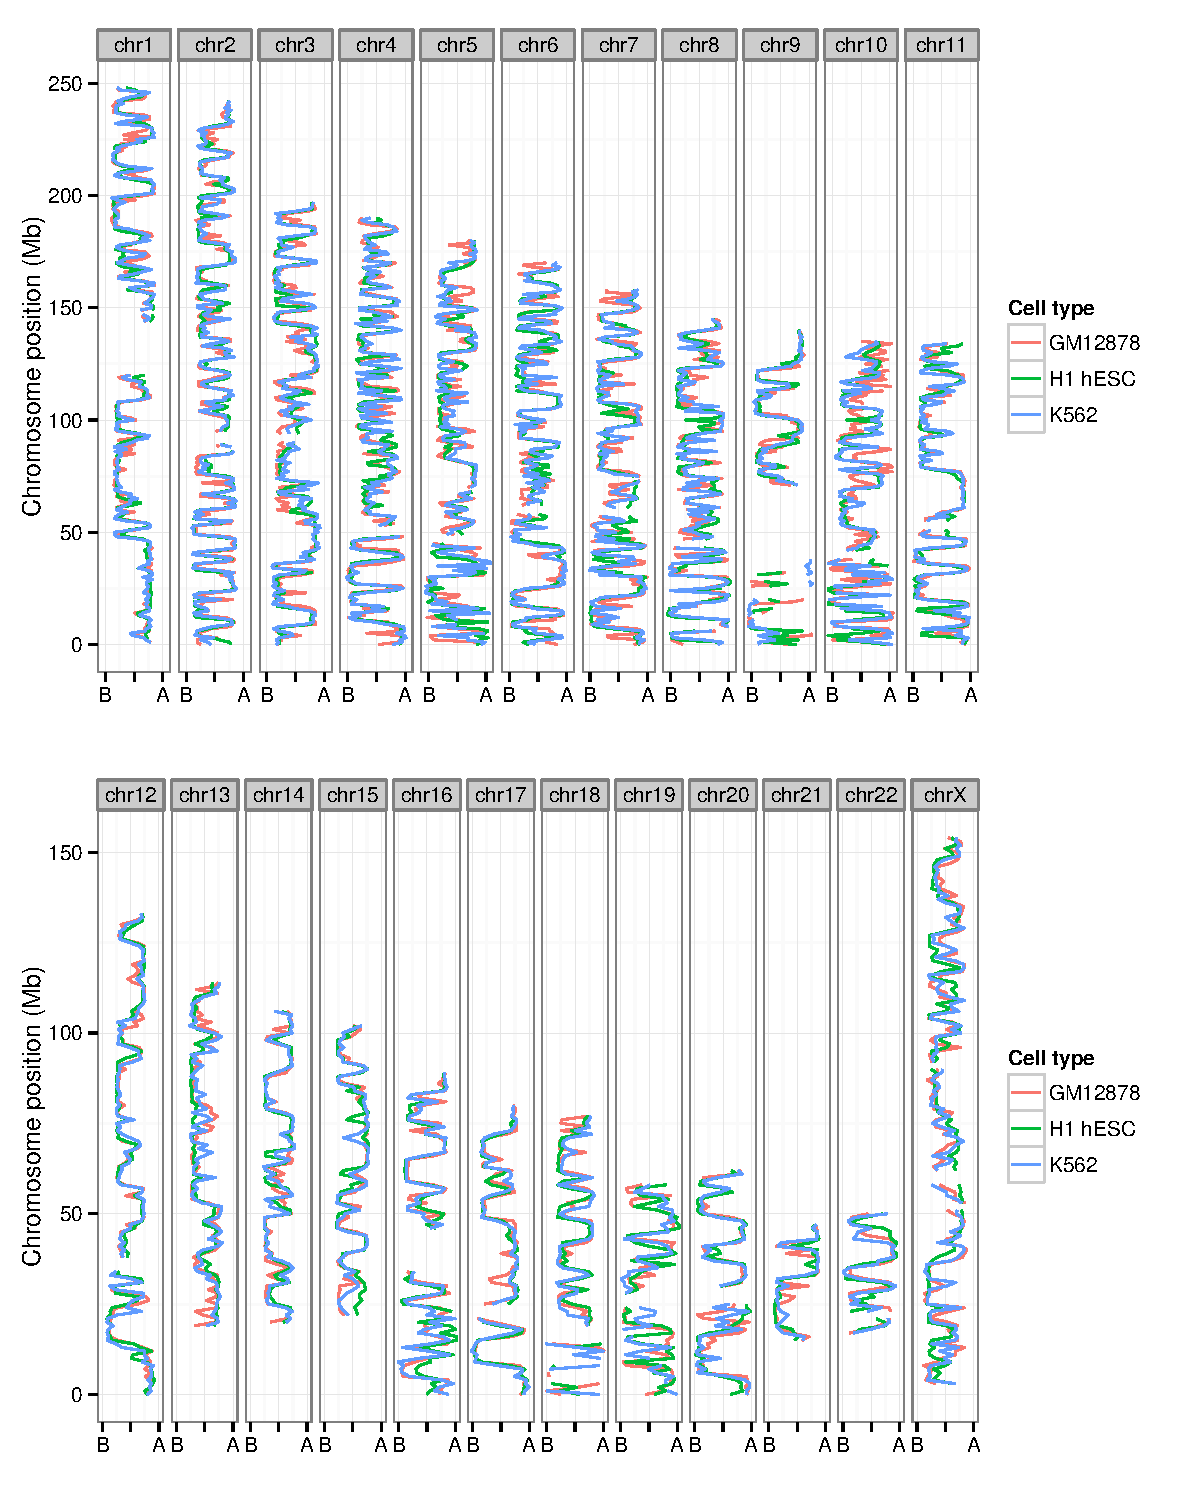
\includegraphics[width=1.2\textwidth]{figs/wiggles.pdf}
\captionsetup{width=\textwidth}
\caption{
{\bf Compartment profiles are observably well-correlated between human cell types and across all chromosomes.}
Caption
}\label{fig:wiggles}
\end{center}
\end{figure} 

This close correspondence also validates our approach of combining these different datasets, and suggests our uniform pipeline is successfully accounting for differences in sequencing depth and other batch effects. The precise correlations of these independent measures are in the interval $R = [.75, .8]$ (Fig. \ref{fig:compactor}; Pearson correlation coefficients, PCC).

\begin{figure}
\begin{center}
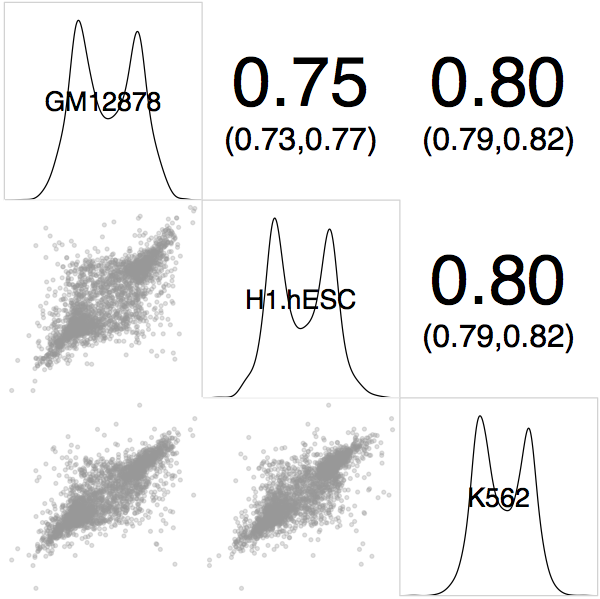
\includegraphics[width=.5\textwidth]{figs/compartment_corr.png}
\captionsetup{width=\textwidth}
\caption{
{\bf Compartment eigenvectors are well-correlated between human cell types}
Megabase resolution compartment eigenvector values are shown in a plot matrix. \emph{Upper triangle}: Pearson correlation coefficients between pairs, with $95\%$ confidence intervals (??); \emph{diagonal} Kernel density estimates of eigenvector values per cell type; \emph{lower triangle}: $x$-$y$ scatterplot of values.
}\label{fig:compcor}
\end{center}
\end{figure} 

\section{Domain calls}

The continuous compartment eigenvector can be used as-is to classify A/B compartments, using positive and negative eigenvector values after first orientating the vector with respect to, for example, PolII Chip-seq data.\cite{Kalhor2012} However, given the definition of compartments as generally broad and alternating domains along a chromosome, often matching other large domains of Lamin association, an improved classification method might penalise the calls of short compartment calls, which may be the result of noise.

For this reason, instead of using raw eigenvector values we consider observed values as emissions from unobserved underlying states. This can be modelled through a Hidden Markov Model (HMM), whereby we first parameterise models of state and their transitions, then infer the most likely state sequence to have emitted our observed data. This unobserved two-state sequence is then used for compartment calls. 

In practice, this acts to de-noise our compartment calls. Where single sign-changes along the series would have resulted in a single-block compartment, these may now be modelled as noisy emissions from a single unobserved state. An examplar region is showing in Fig 

% figure showing raw eigs with hmm calls
\begin{figure}
\begin{center}
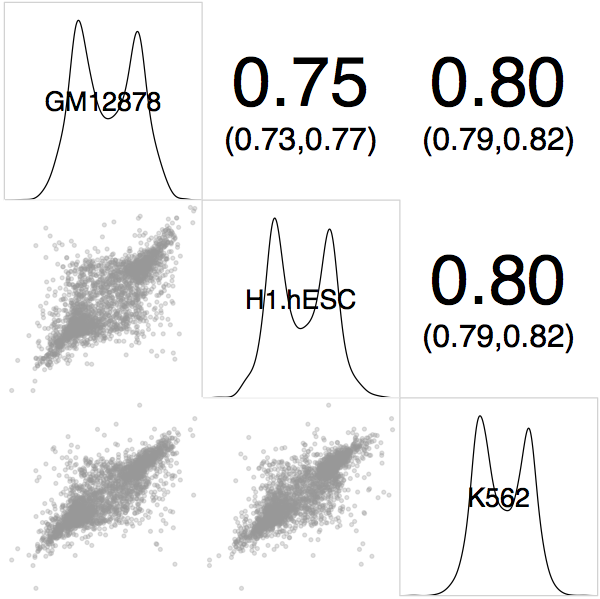
\includegraphics[width=.5\textwidth]{figs/compartment_corr.png}
\captionsetup{width=\textwidth}
\caption{
{\bf Compartment eigenvectors are well-correlated between human cell types}
Megabase resolution compartment eigenvector values are shown in a plot matrix. \emph{Upper triangle}: Pearson correlation coefficients between pairs, with $95\%$ confidence intervals (??); \emph{diagonal} Kernel density estimates of eigenvector values per cell type; \emph{lower triangle}: $x$-$y$ scatterplot of values.
}\label{fig:compcor}
\end{center}
\end{figure} 

% figure showing size distributions of Hi-C domains

\section{Variable regions}
% investigate those regions which are "flipped"

Despite the vast majority of the genome being in matched chromatin compartments, there are also regions of disagreement. Reasons for observable differences include technical errors and bias, but also more interesting functional explanations, where cell-type specific activation or repression is reflected in changes in higher order structure.








% fig 1.

\section{Nuclear positioning}



%\ifstandalone
\begin{small}
\bibliography{/Users/benmoore/Documents/library,/Users/benmoore/Documents/customrefs}
\end{small}
%\fi

\end{document}


\documentclass[a4paper,11pt,oneside]{book}

% packages 
\usepackage{arsclassica}    % fancy layout
\usepackage[english]{babel}\addto{\captionsenglish}{\renewcommand{\bibname}{References}}
\usepackage{caption}         % figure captions
\usepackage[square,numbers,super,sort&compress]{natbib}  % bibliography style
\usepackage[cc]{titlepic}    % enable logo on title page
\usepackage{graphicx}       % logo related

\usepackage{standalone}

% bibliography
\bibliographystyle{../thesis}

% title setup
\title{ \vspace{3in} Unravelling higher order genome organisation {\small [working
    title]} \\ \vspace{2em} {\large {\bf Results 2} Predictive modelling } }
\author{Benjamin L. Moore}
\titlepic{\vspace{2.2in} 
\includegraphics[width=\textwidth]{/Users/benmoore/hvl/1yrReport/figs/igmm.png}}

\begin{document}

\maketitle

\chapter{Integrative modelling as a tool to explore biological systems}
\vspace{2em}

\section{Introduction}
Large-scale chromatin data has recently been produced by multiple
consortia, most notably the ENCODE\cite{Gerstein2012} and NIH
Roadmap Epigenomics\cite{Bernstein2010} projects. The breadth and depth of this new
data offers unprecedented opportunities to further our understanding
regarding the fundamental biology of the chromatin landscape. While many histone
modifications can now be quantified experimentally,\cite{Nikolov2012, Sajan2012, Ernst2011} an integrated
understanding of general mechanisms underlying the cause or effect of
these marks lags behind. A 2011 opinion piece asked
the question ``Histone modification: cause or
cog?''\cite{Henikoff2011} and speculated that nucleosome modifications
could be by-products of transcription machinery, as opposed to
the ``histone code'' hypothesis which suggests that histone
modifications are placed to direct alterations in chromatin
state. This latter hypothesis is often tacitly invoked in the
chromatin literature, wherein a mark may be described as
``repressive'' or ``activating'' despite only the observation of a
correlative relationship.\cite{Henikoff2011} Similarly, the interplay
between locus-level factors and higher-order organisation of
chromatin, while known the be an important factor in
transcription, remains poorly understood mechanisatically.\cite{Li2011} 
% Colin's sentence:
However, the recent flood of data from high throughput sequencing technologies have provided fascinating new glimpses of the ways chromatin and transcription are functionally related.

Recent studies have shown convincingly that local chromatin state
measurements can accurately predict expression levels of genes on a
genome-wide basis. Tippmann \emph{et
  al.},\cite{Tippmann2012} designed a linear model to predict
steady-state mRNA levels in mouse (\emph{Mus musculus}) embryonic stem
cells based on just four predictors: 3 histone modifications
(H3K36me3, H3K4me2 and H3K27me3) and
Pol-II occupancy. Remarkably, the linear model was found to explain
84.6\% of an estimated 91\% maximal variance that could be explained
(as calculated through a detailed determination of noise). An additional
finding of this study was that mRNA half-life and microRNA mediated
transcript degradation both had relatively minor influence on
steady-state mRNA levels, with the authors concluding that``the lion's
share of regulatory contribution is at the level of mRNA synthesis and
predictable from chromatin alone.''\cite{Tippmann2012} An independent
study used a similar regression modelling approach to chromatin
and transcription factor data and again
concluded that models built with histone modifications and chromatin
accessibility data were almost as accurate as those which also
included binding data for 12 transcription factors.\cite{McLeay2012a} 

A recent key study from the ENCODE consortium used chromatin (ChIP-seq) datasets to predict gene expression in a range
of cell types as measured by a variety of experimental techniques.\cite{Dong2012} The authors here developed a
two-stage model which first attempts to classify each transcription
start site (TSS) into an `on' or `off' state using a powerful ensemble
classifier technique called Random Forests (RF). The second stage of the
model used the same range of histone modifications as regressors in a
simple linear modelling framework to quantify predicted
expression. This approach proved very successful, producing a
median Pearson correlation coefficient ($r$) between predicted and
empirical expression levels using 10-fold cross-validation of
$0.83$ across all cell lines and expression level
technologies.\cite{Dong2012} Additionally, this study highlighted cap
analysis of gene expression (CAGE) as the 
technology, relative to RNA-Seq and RNA-PET, which produced the most
predictable expression response. CAGE uses 5$^\prime$ capped transcripts to
generate short, specific tags which precisely identify TSS positions as well as
quantifying the abundance of a given transcript.\cite{Shiraki2003, Kodzius2006}

These recent publications highlight the importance and relevance of
advancing our understanding of chromatin biology through a model-based
approach. Each of these existing models however, treats expression
levels as stationary outcome in each cell type and ignores any temporal
dynamics. The huge amount of novel timecourse CAGE data 
produced by the FANTOM5 consortium\cite{fantom5} puts us in an ideal
position to investigate how chromatin influences transcription beyond a
simple single-point response and move towards a more complete
understanding of the drivers of transcriptional flux.

\section{Reproducing Dong \emph{et al.} }

Following on from Dong \emph{et al.},\cite{Dong2012} I first
reimplemented the published ENCODE modelling framework to ensure I could
replicate their results. In doing so I was also able to analyse the
strengths and caveats of their approach; surprisingly the two-step classification
then regression (firstly assessing a gene as `on' or `off' and then
predicting its expression level) added little additional accuracy relative to a simple
linear regression model 
(Fig. \ref{fig:TwoStepvsSimple}). 

\begin{figure}
\begin{center}
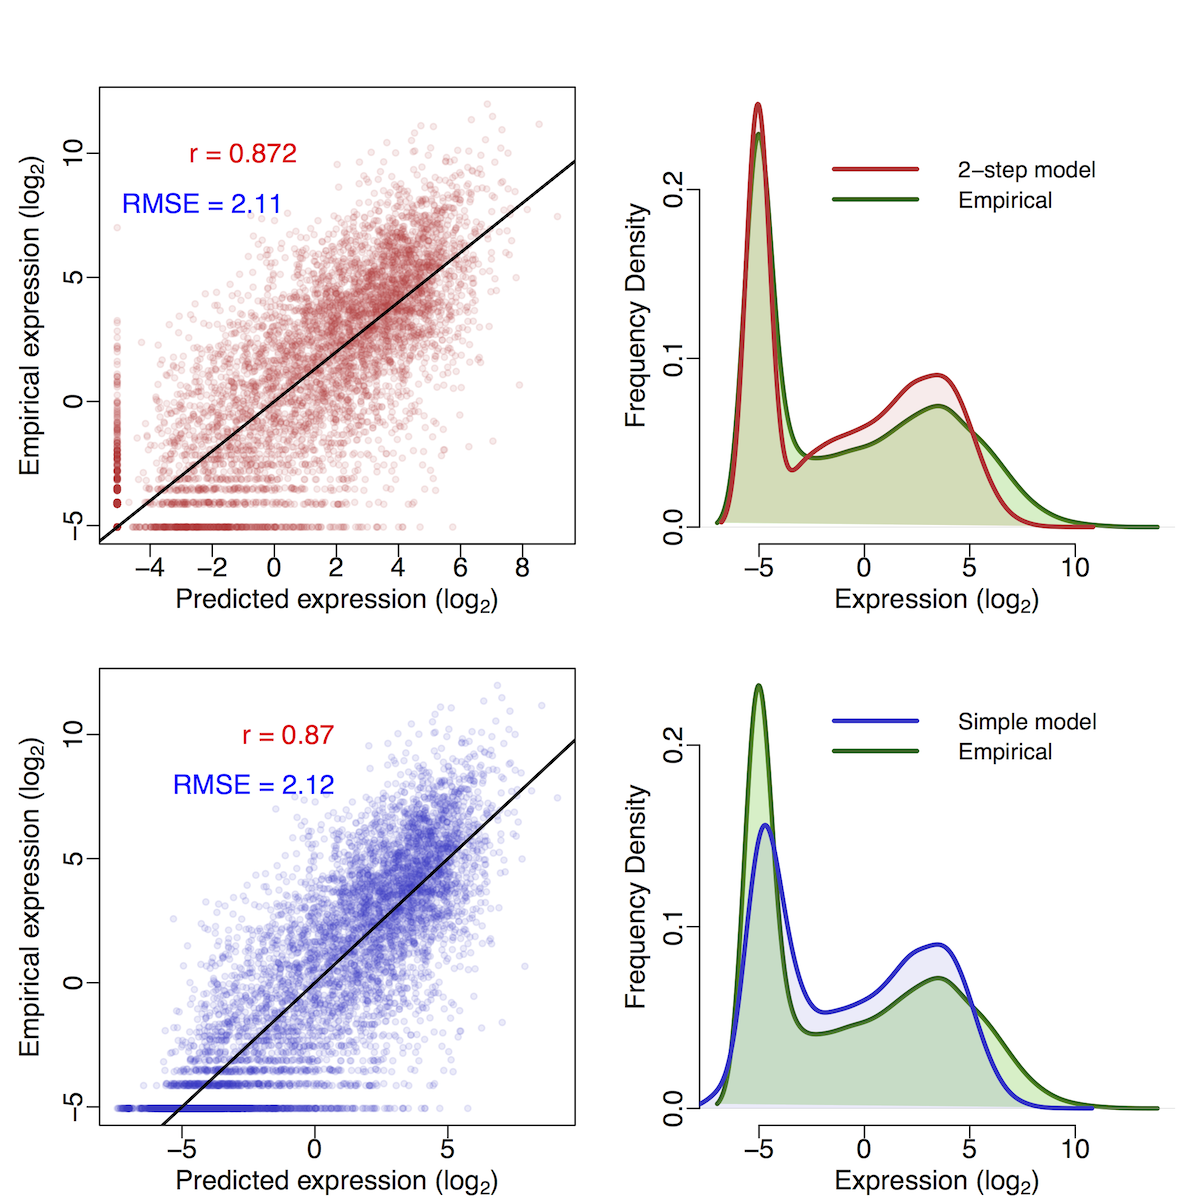
\includegraphics[width=.7\textwidth]{figs/improvedDongPlot.png}
\captionsetup{width=\textwidth}
\caption{Comparison of classification-regression model (\emph{upper})
  with simple linear regression model (\emph{lower}) recalculated following Dong
  \emph{et al.}\cite{Dong2012} Scatterplots of predicted against empirical
  $\log_2$ reads per million (RPM) expression values for both methods are shown (\emph{left})
  along with frequency distributions of predicted and observed
  expression levels (\emph{right}). Scatterplots are annotated with
  Pearson's correlation coefficient (\emph{r}) and the root mean
  squared error (RMSE); the black trendlines describe $y =
  x$. Following 10-fold cross validation, overall correlation
  coefficients were: linear model $0.87 \pm 1.77 \times 10^{-5} $;
  Two-step model $0.872 \pm 9.89 \times 10^{-5} $. All correlations
  were statistically significant with $p < 1 \times 10^{-15}$ under the assumption of a
  $t$-distributed $r$ with $d.f. = 7998$.
}\label{fig:TwoStepvsSimple}
\end{center}
\end{figure} 

An innovative element of Dong \emph{et al.}'s modelling approach is the `bestbin' method of matching
chromatin measurements to the expression of a given TSS. This strategy
first bins normalised signal intensities into $40 \times 100$ bp bins
encompassing 4 kbp around the TSS, and adds an additional bin representing the remaining
gene body. Then the correlation between
the signal of a given mark and the expression of a TSS across all
genes is measured --- the bin producing the highest correlation is
designated as the `bestbin' and that bin's normalised ChIP-seq signal intensity in then
taken forward for the full model. This was shown to raise
the correlation (between predicted and observed expression) by 0.1 in
the simple regression model, an increase in accuracy of almost $13\%$,
relative to simply taking the average value across all
bins.\cite{Dong2012} 

\begin{figure}
\begin{center}
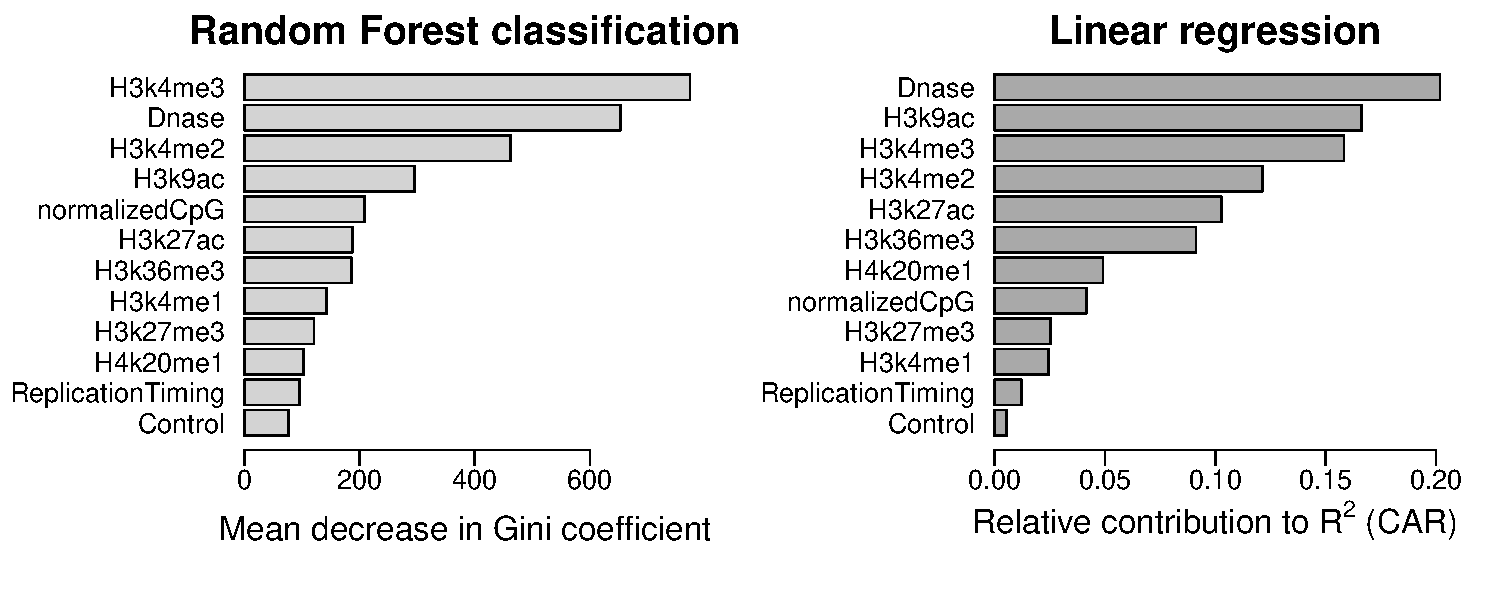
\includegraphics[width=\textwidth]{figs/Dong_relImp_Horiz.pdf}
\captionsetup{width=.9\textwidth}
\caption{Relative importance metrics for variables in both the
  classification (\emph{left}) and regression (\emph{right}) stages of
  my reimplementation of Dong \emph{et al.}'s two-step
  model.\cite{Dong2012} The additional variable `ReplicationTiming'
  shows the influence of $\log_2 (early/late)$ replication timing ratio measured in the BG02 ESC cell type;\cite{Ryba2010}
  H1 hESC data was not available but these higher-order measurements
  appear to be largely conserved across cell-types.\cite{Chambers2012}
  For details of CAR $R^2$ decomposition, see Zuber and Strimmer (2010).\cite{Zuber2011}
}\label{fig:relimp}
\end{center} 
\end{figure} 

I attempted to improve the accuracy of predicted expression values
produced by Dong \emph{et al.} through two methods: increasing the number of informative
regressors and increasing the complexity of the model by adding
interaction terms and/or non-linear components. While Dong \emph{et
  al.} included broad coverage of different histone modifications,
they did not investigate the impact of higher-order
chromatin data. For this reason, I matched the TSS positions used in
Dong \emph{et al.} with previously-published genome-wide replication
timing ratios measured in BG02 ESCs.\cite{Ryba2010} I then used these values as an additional
regressor in both the two-step classification regression model and the
simple linear model but saw no significant improvement in either
model's accuracy. The reasons for this are likely that the 
data were relatively low-resolution (1 megabase blocks), from a
imperfectly matched cell line and also that
the Dong \emph{et al.} model is already achieving such accurate
results that they must already be accounting for most of the maximal
explainable variance in gene expression given experimental and
biological noise. With this in mind, additional regressors would be
expected to yield diminishing returns. However, on closer examination,
the replication timing data
appeared only slightly more informative than the control ChIP-seq input
measurements when evaluated with relative importance metrics
(Fig. \ref{fig:relimp}), implying that large-scale chromatin domains
and long range interactions
do not have significant influence on the expression of the genes resident within them. It would
be of interest to investigate this further should more detailed higher order
data become available. For example Hi-C interaction matrices have been
calculated in the H1 cell line\cite{Dixon2012} and these could be
compressed to principle component eigenvectors as has been done with
other cell lines.\cite{Lieberman2011}

\section{Modelling FANTOM5 CAGE timecourse data}
Using unpublished FANTOM5 data and the approach established above, I next attempted to model gene
expression at timepoint zero ($t_0$) of a differentiation timecourse of Human
H1 embryonic stem cells (H1 hESC) to CD34+ hematopoietic stem
cells.

% How did I do this?:
% 1) Take robustly mapped CAGE clusters -> Entrez Gene IDs
% 2) Select the strongest expressed CAGE cluster
% 3) Either a) use this as a TSS or b) map to closest annotated TSS
The first stage of the analysis was to map each CAGE cluster to a
representative TSS. FANTOM5 robust gene mapping\cite{fantom5}
provided corresponding Entrez Gene IDs for gene-associated CAGE
clusters, and I selected the most expressed cluster to represent the
expression level of its mapped gene. I then compared these to Ensembl
TSS annotations (v69) and
discarded those tag clusters centered on a point $>50$ bp from an annotated
TSS associated with the mapped Entrez Gene ID, thereby removing enhancers and other non-genic transcribed
regions.

Next I retrieved a number of genome-wide histone modification datasets
from the ENCODE and
NIH Roadmap consortia which were measured in H1 hESC cells, taking these to be
reflections of the chromatin state $t_0$. I implemented the
previously-described `bestbin' strategy\cite{Dong2012} to objectively
select the most-correlated binned signal for each chromatinH1 hESC
mark. Additionally, I analysed the stability of chosen bestbins by
calculating them on 200 sets of 1000 randomly selected TSS samples (with each sample
representing approximately $8\%$ of the dataset) and the result is
shown in Figure \ref{fig:bestbin}.

\begin{figure}
\begin{center} 
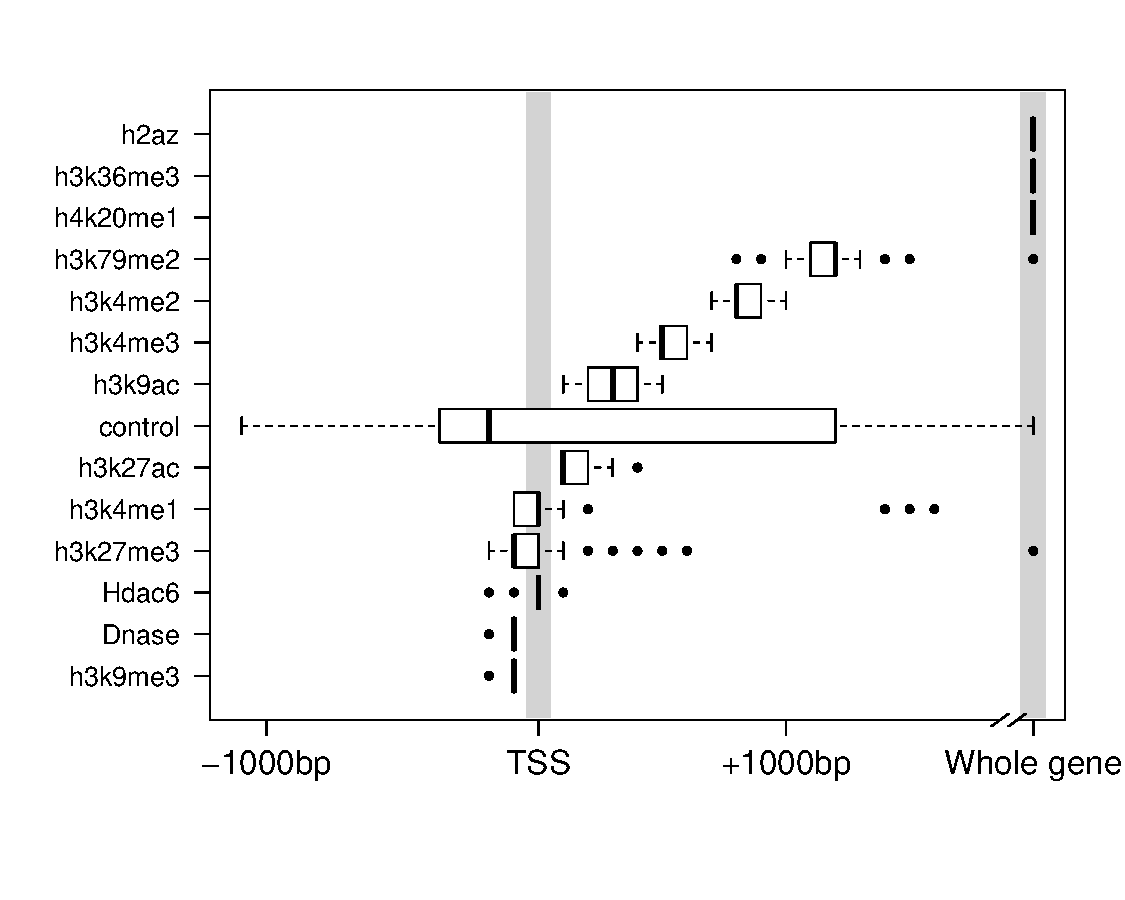
\includegraphics[width=.9\textwidth]{figs/bestbinSummary.pdf}
\captionsetup{width=\textwidth}
\caption{Distributions of bestbin locations relative to the
  TSS. Bestbins were selected for normalised ChIP-seq
  signal intensities for 10 histone marks, the
  H2A.Z histone variant, Hdac6 histone deacetylase, Dnase
  hypersensitivity and a ChIP-seq input chromatin control. Bins analysed
  extended 2 Kb flanking the TSS, but more distal bins were
  never selected and hence are not shown. `Whole gene` represents the
  averaged signal intensity from TSS to transcript end site, as
  defined by Ensembl Genes v69.
}\label{fig:bestbin}
\end{center}
\end{figure} 

This result shows that bestbin selections are often consistent, indicating there are predictably informative regions
relative to a TSS for each chromatin factor (Fig. \ref{fig:bestbin}). Furthermore, the selected
bestbins match known biological mechanisms; for example the H3K36me3
mark's bestbin is consistently the whole gene measurement and this
mark is known to be enriched in actively transcribed
exons.\cite{Tippmann2012, Kolasinska-Zwierz2009, Schaft2003} 

Having matched a variety of genome-wide H1 hESC chromatin datasets
to the FANTOM5 timecourse expression data, I then built a regression
model using a Random Forest (RF) approach.\cite{Breiman2001} This method outperforms a simple
linear model in my initial comparisons and is able to capture non-linear relationships as well
as interactions without them being explicitly specified.\cite{Diaz2006}

\begin{figure}
\begin{center} 
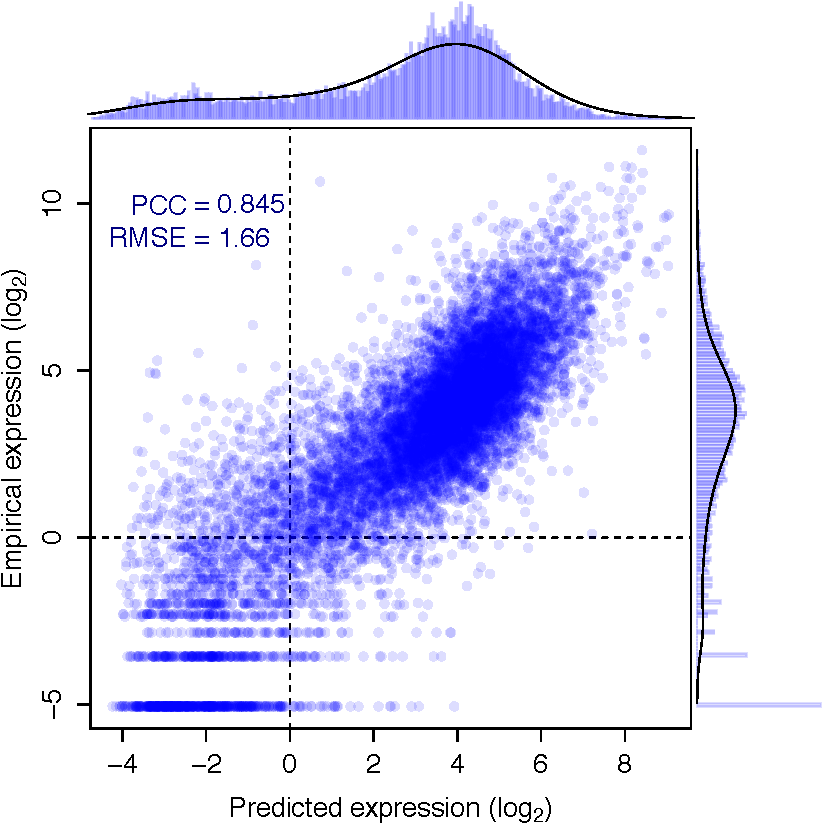
\includegraphics[width=.6\textwidth]{figs/RandomForest_10CV_50d.pdf}
\captionsetup{width=\textwidth} 
\caption{Evaluation of RF model predictions ($x$-axis) against an independent
  test set ($y$-axis). The distributions of predicted and empirical
  expression values are shown opposite their
  respective axes. Pearson's correlation coefficient ($r$) and the root
  mean-squared error (RMSE) are also shown (\emph{inset}).
}\label{fig:model}
\end{center} 
\end{figure} 

Figure \ref{fig:model} shows the resulting predictions of a
preliminary RF model against the actual recorded expression over a
test set of approximately 11000 TSS. This model was built with 15
predictors including control ChIP-seq input, though some of these could be
removed without loss of accuracy. The model predictions evluated with
10-fold cross validation show a
significant correlation with measured CAGE levels ($ r = 0.845\pm
1 \times 10^{-4}$; $t_{10868} = 164.4$,
$p < 2 \times 10^{-15}$), and the model is able to explain around
$71\%$ of the variance in the expression response (for comparison a
linear model resulted in $r = 0.825 \pm 3.2 \times 10^{-5}$; $t_{10868} = 152.2$,
$p < 2 \times 10^{-15}$).

This result is worse than that of Dong \emph{et al.}
who achieved cross-validated correlation coefficients of up to $0.9$,
but it is roughly equal to their median test set correlation of
$0.83$.\cite{Dong2012} The RMSEs, when normalised by the range of
observed values, compare more favourably ($0.11$, compared with Dong \emph{et al.}'s: $0.14$). A possible explanation for this decrease in
accuracy is that while both chromatin data and expression timecourse
were measured in H1 hESC cells, the experiments took place at
different institutes and likely using differing protocols and cell cultures. For comparison, a previous study using chromatin
measurements from a number of different sources to predict expression
in a matched cell-type reported a predictive correlation of 0.77.\cite{Karlic2010} Additionally, Dong \emph{et al.} implemented a pseudocount
optimisation step whereby an additional count added to each binned signal
intensity prior to log transformation was optimised to maximise
expression correlation. In the model presented above, a fixed
psuedocount of $1$ was used to avoid introducing positive bias towards
higher correlation. Another difference between the two approaches is
our use of a single-step model; Dong \emph{et al.} found a small
increase in correlation using their classification-regression approach
but with the model implemented herein (Fig. \ref{fig:model}) this approach gave no obvious advantage (for
example, $r
= 0.834 \pm 0.007$, $\textrm{RMSE} = 1.77$ when applied to the same test and
training data used in Fig. \ref{fig:model}).

Having built a reasonable model of $t_0$ expression, the next stage of
this preliminary analysis was to consider successive timepoints. In the
available CD34+ differentiation dataset, this consisted of expression
data recorded at three
timepoints (days 0, 3 and 9---hereafter $t_0$, $t_3$ and $t_9$
respectively). However genome-wide expression
was highly correlated between each of these timepoints (Pearson correlation coefficients: $t_0, t_3 = 0.911; ~t_0,t_9 =
0.913; ~t_3,t_9 = 0.977$), and this high correlation meant that the
genome-wide model performed essentially equally well regardless of the
expression timepoint it was trained or tested on. In future analyses, higher-resolution timecourses may offer
more interesting variation or alternatively genes that remain invariant
throughout the timecourse could be filtered out of the dataset. 

\section{Modelling higher order chromatin}

Accurate predictive modelling of transcription in a variety of cell types offered several novel insights into the internal between histone modifications and transcription factors with transcriptional machinery, and advanced a quantitative explanation of the degree to which correlated features are informative. It is of interest then, to test whether this approach can be applied to other data, such as the reprocessed higher order chromatin data assembled in this work (Chapter 1).

Previous publications have identified several correlates which track compartment eigenvector profiles to varying degrees,\cite{Lieberman2009, Imakaev2012} yet to date these relationships have not been quantitively investigated. The above-described modelling framework offers a statistical approach to understanding the drivers of these observed correlations.

\subsection{Predictive model}

We built Random Forest regression models (see Methods XX) to predict compartment eigenvector profiles genome-wide in three human cell types. Models were found to have high predictive accuracy, with Pearson correlation between predicted and observed compartment eigenvectors in the range of 0.82--0.75 (Fig. \ref{fig:modelres}), comparable to that achieved by Dong \emph{et al.}\cite{Dong2012} in the prediction of transcription.

\begin{figure}
\begin{center} 
\makebox[\textwidth][c]{ 
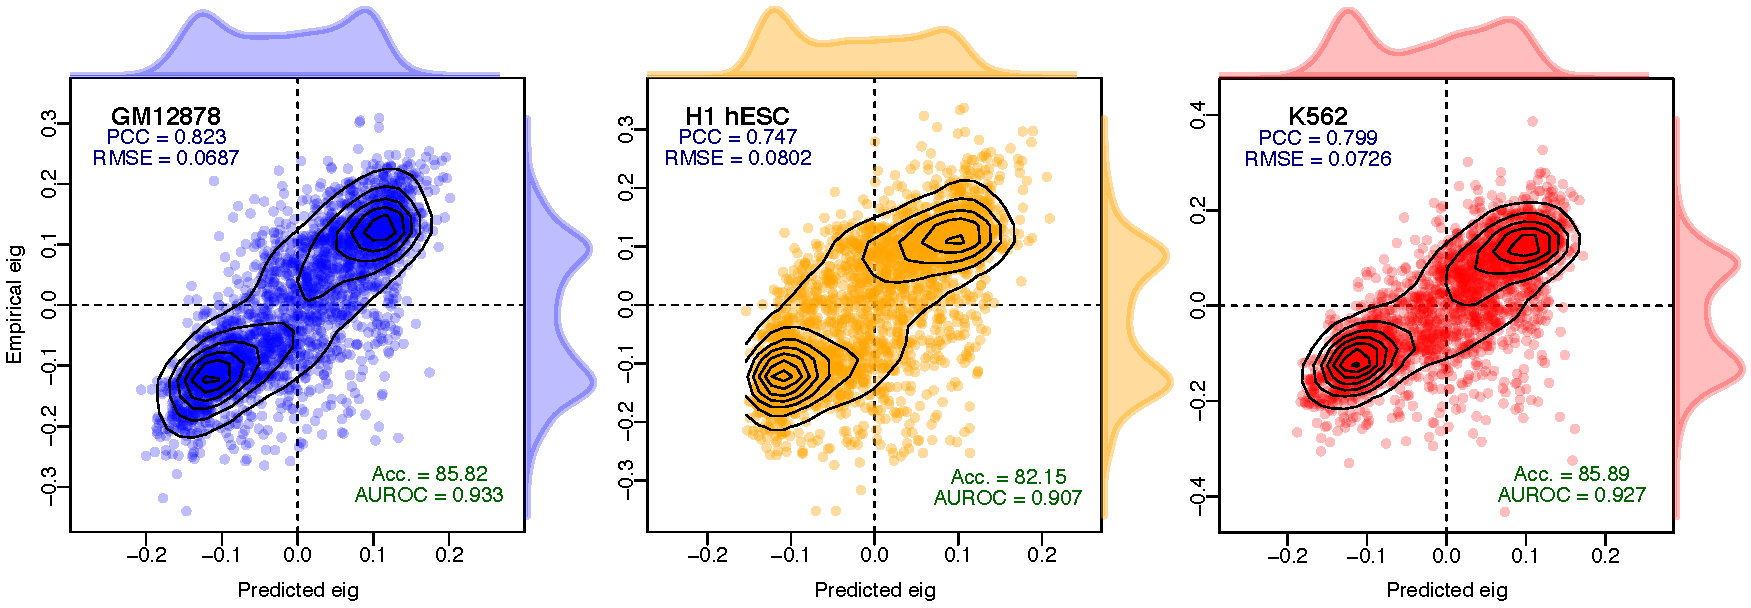
\includegraphics[width=1.3\textwidth]{figs/modelres.pdf}
}
\captionsetup{width=\textwidth} 
\caption{ {\bf Compartment eigenvector model predictions are highly correlated with observed values.}  Pearson correlation coefficient (PCC) and root mean-squared error (RMSE) report the degree of success of the regression model, whereas accuracy (Acc.) and area under the receiver operating characteristic (AUROC) give the classification accuracy of binarized outcomes.
}\label{fig:modelres}
\end{center} 
\end{figure} 

Our predictive models were also assessed in terms of classification performance, i.e. did the model correctly assign each block to an active "A" or inactive "B" compartment. As with regression, our Random Forest models achieved high classification accuracy with upwards of $80\%$ of the all genomic bins correctly assigned in each cell type (Fig. \ref{fig:modelres}). 

This predictive performance underlines the strong connection between locus-level features and higher order chromatin structure previously noted by \citet{Lieberman2009} Given such highly-predictive models can be generated, it is then of interest to dissect said models in an attempt to understand the nature of this captured relationship.

\subsection{Cross-application}

High predictive accuracy on cell type specific models could be the result of ``over-fitting". In machine-learning, over-fitting refers to the point at which parameters are being optimised to capture noise within a feature set, as well as signal, thereby giving an overoptimistic model performance which would not generalise to another featureset with different noise profiles.

To test if over-fitting was causing our high observed accuracy, we cross-applied models learnt in one cell type to unseen input data from each of the other two cell types under study. If predictive accuracy is a lot lower on unseen data, this lends evidence to the idea that our models may be overfitted to their respective cell types. Conversely, it could be the case that biologically-distinct mechanisms are in place that differ between cell types, preventing a simple cross-application.

\begin{figure}
\begin{center} 
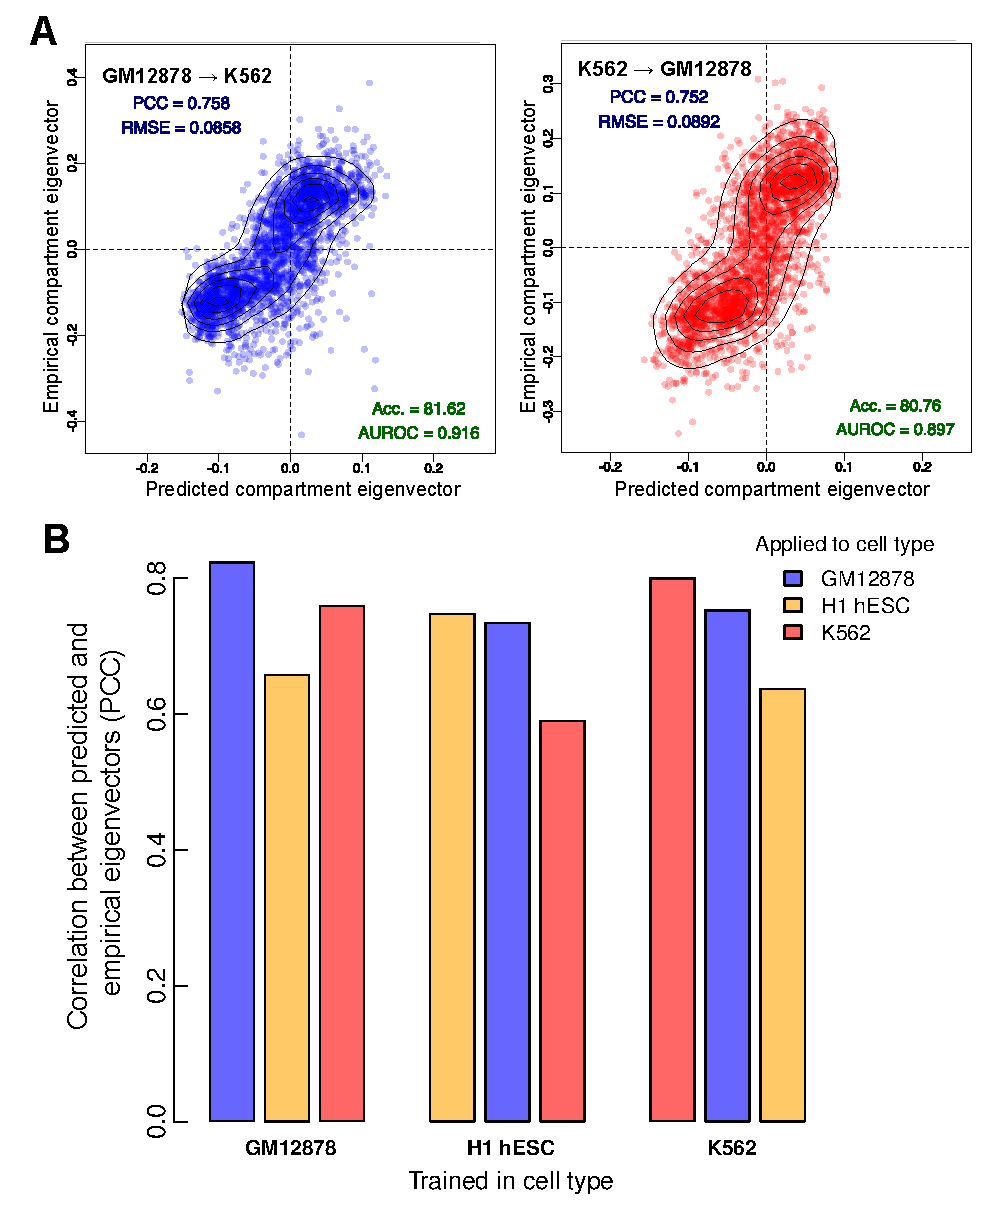
\includegraphics[width=.7\textwidth]{figs/xapp.pdf}
\captionsetup{width=\textwidth} 
\caption{ {\bf Models of higher order chromatin structure learned in one cell type can be cross-applied to two others }
 Each model, trained in one cell type, was applied to the chromatin feature datasets from the other two cell types. (A) The GM12878 model achieved high accuracy when applied to K562 features (PCC $= 0.76$), as did the reciprocal cross (PCC $= 0.75$). (B) In each case, predictive accuracy decreased on cross-application but there remains significant agreement between predicted and empirical values. Acc., accuracy; AUROC, area under the receiver operating characteristic curve; PCC, Pearson correlation coefficient; RMSE, root mean-squared error.
}\label{fig:xapp}
\end{center} 
\end{figure} 

We found cross-application between cell types was possible and with similarly-high levels of accuracy (Fig. \ref{fig:xapp}). This gives good evidence not only that are models are not overfitting to cell-type specific noise, but also that there exist broad rules linking chromatin conformation and locus-level feature aggregation. The cross-application suggests there exists enough commonalities for compartment profile predictions to transcend the cell-type specific biology inherent to an embryonic stem cell or differentiated lymphoblast.

\subsection{Variable importance}

\begin{figure}
\begin{center} 
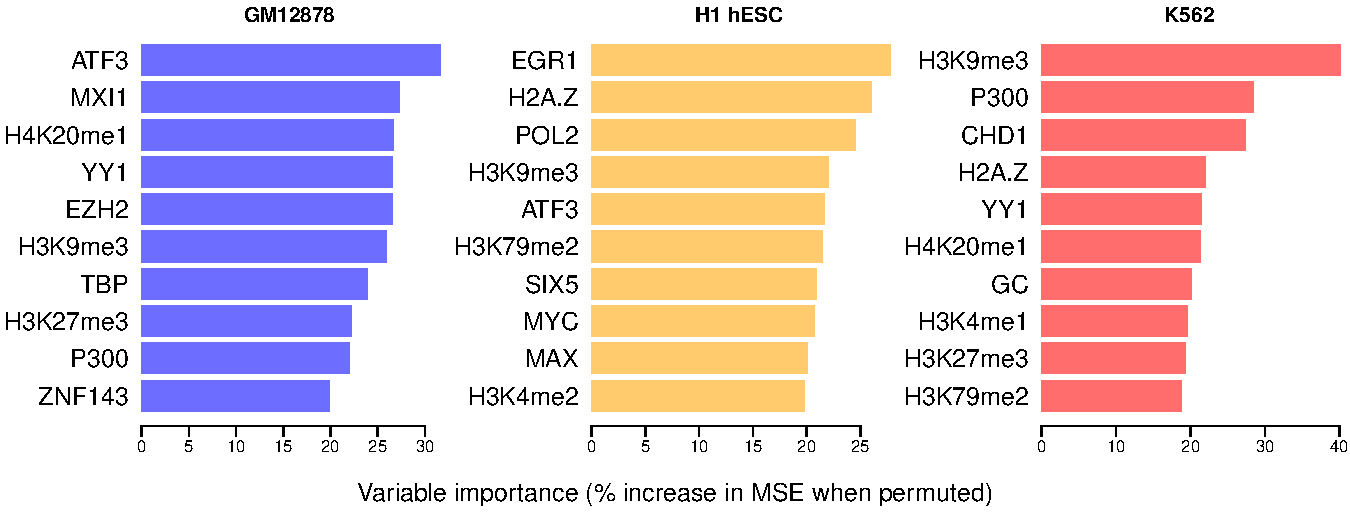
\includegraphics[width=\textwidth]{figs/varimp.pdf}
\captionsetup{width=\textwidth} 
\caption{ {\bf Variable importance per cell type specific model. }
Variable importance for each Random Forest model was measured in terms of percentage increase in mean squared error when permuted (Methods XX) and the top 10 ranking variables are shown for each model.
}\label{fig:varimp}
\end{center} 
\end{figure} 

Having built accurate predictive models, we next dissect the relative variable contributions made from our range of input features and compare these across cell types. An overview on the top 10 most highly-ranked features in cell type specific models shows some agreement but also substantial differences between cell types (Fig. \ref{fig:varimp})

Only one input feature, H3k9me3, is present in the top 10 most important variables of each model (Fig. \ref{fig:top10venn}). H3k9me3 is one of the few features to be negatively correlated with compartment eigenvectors (Fig XX). Of those shared between two cell type models, H3k27me3 is also a repressive mark and deposited by polycomb repressive complex 2 (PRC2)\cite{Vizan2014} while H2A.Z is a histone variant again linked to polycomb-regulated genes and essential for embryonic development.\cite{Creyghton2008} Furthermore EZH2, the catalytic subunit of PRC2,\cite{Deb2014} is also included in the feature set but only highly ranked in the GM12878 cell type model. These biological relationships between variables may help explain the observed differences between models: different representatives of correlated clusters of input variables may be being selected in each model (see Section \ref{sec:corrinputs}).

\begin{figure}
\begin{center} 
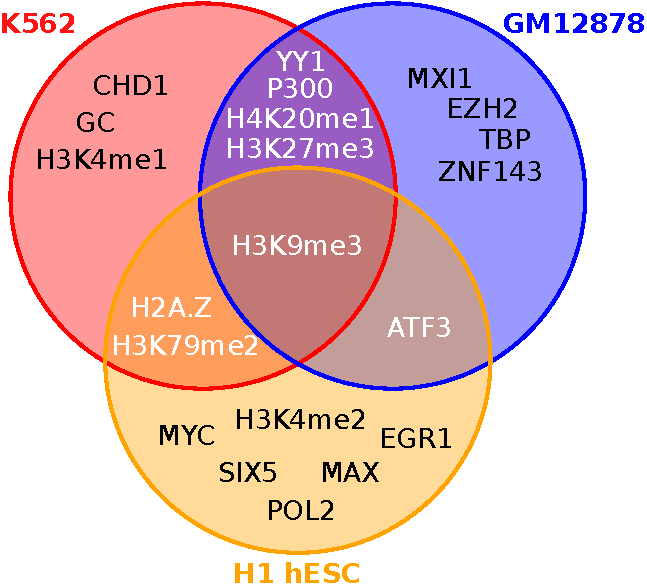
\includegraphics[width=.5\textwidth]{figs/top10venn.pdf}
\captionsetup{width=\textwidth} 
\caption{ {\bf Intersections of the top 10 ranked variables in the cell type specific models. }
Venn diagram illustrating intersections between sets of ten most influential variables per cell type specific Random Forest regression model of compartment eigenvector (Fig. \ref{fig:varimp}).
}\label{fig:top10venn}
\end{center} 
\end{figure} 

To asses the significance of observed intersections (Fig. \ref{fig:top10venn}), the variable selection process could be modelled with, for example, a multivariate hypergeometric distribution or via simulation. Simulation was used here for simplicity: each intersection was calculated under $10,000$ variables draws with uniform distribution and empirical $p$-values were then calculated accordingly. Under the assumption that variables are ranked independently in each cell type, drawing at least one variable in all three cell types would be expected by chance (simulated $p$-value of $0.6$). Similarly, the overlaps between pairs of cell types is within the range of expectation (probability of 7 or more variables appearing in exactly two sets: $0.39$). Hence these data suggest the top 10 most influential variables are not significantly more alike across the three cell-type specific models than expected by chance, however ten is an arbitrary cutoff, and many of the rankings are based on small differences in variable importance, thus could be unstable between multiple generations of stochastic Random Forest models.

\begin{figure}
\begin{center} 
\makebox[\textwidth][c]{ 
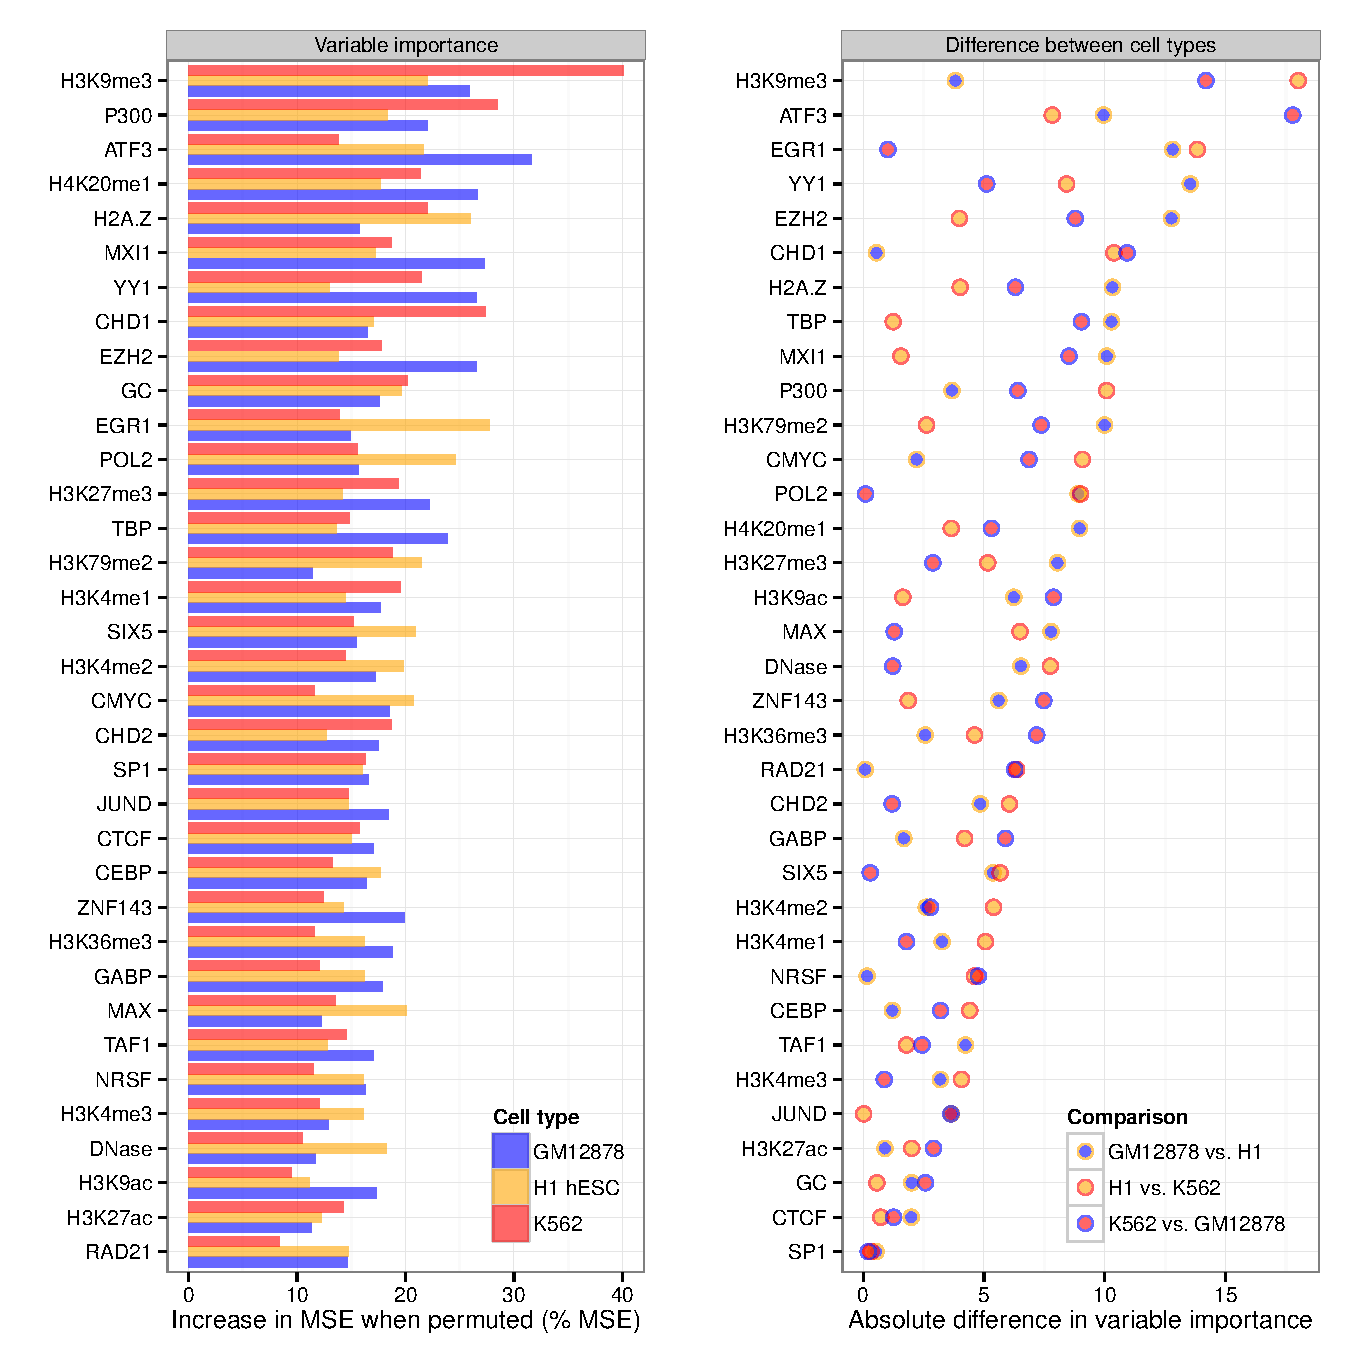
\includegraphics[width=1.2\textwidth]{figs/varimp_diff.pdf}
}
\captionsetup{width=\textwidth} 
\caption{ {\bf Variable importance per cell type specific model. }
Placeholder
}\label{fig:varimp_diff}
\end{center} 
\end{figure} 

In addition to rankings, raw variable importance metrics can be compared between cell-type specific models (Fig. \ref{fig:varimp_diff}).

% figure showing e.g. how individual var regresses against eigen (Egr1compare.pdf)

\subsection{Importance of resolution}

Thus far models were built at 1 Mb resolution, but if we are capturing true biological relationships we would expect these to hold at higher or lower resolution. To test this, models leaned at 1 Mb resolution were applied to feature sets binned at 100 kb, an order of magnitude higher resolution.

\begin{figure}
\begin{center} 
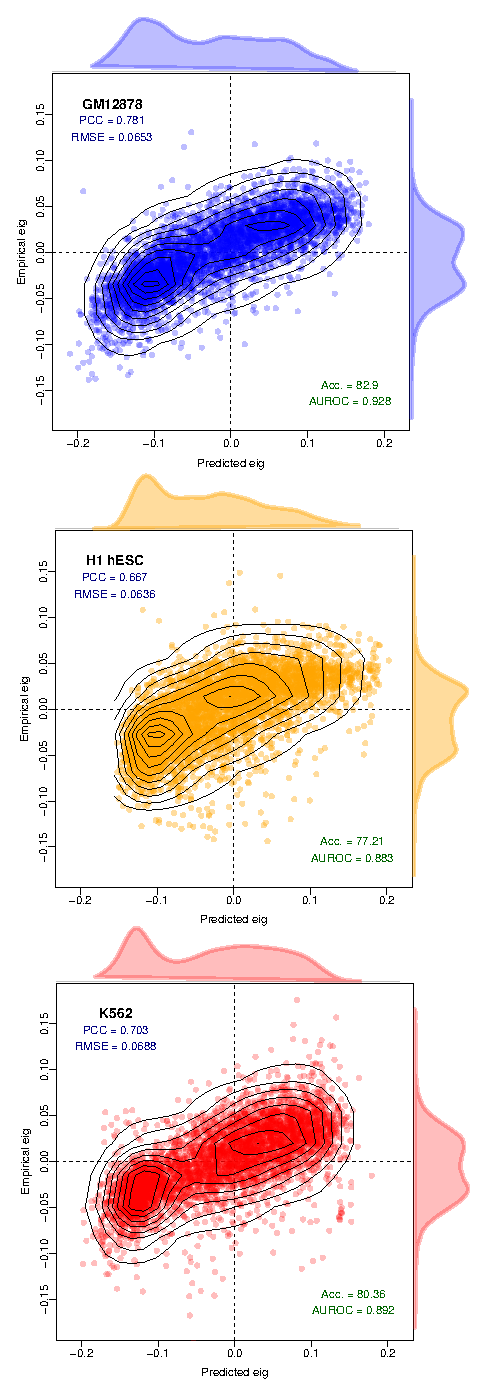
\includegraphics[width=.6\textwidth]{figs/100kb.pdf}
\captionsetup{width=\textwidth} 
\caption{ {\bf Models learned at 1 Mb resolution can be applied to higher resolution datasets. }
Despite having been trained on low resolution training sets, the Random Forest models generated can successfully predict compartment eigenvectors at higher resolution (100 kb, a $10\times$ zoom). Eigenvectors at a higher resolution than this do not necessarily reflect A/B compartmentalisation.
}\label{fig:100kb}
\end{center} 
\end{figure} 

Model accuracy when applied to higher resolution input features proved to be similarly high, with empirical PCC being $88$ to $95\%$ as high as that at 1 Mb native resolution (Fig. \ref{fig:100kb}).

Note however, there is some indirect leakage between test and training set when 100 kb bins have been used in aggregate in learning the 1 Mb models. Nevertheless, sustained accuracy is evidence that our models are not resolution-sensitive, and could likely be applied to higher resolutions than the 1 Mb predominantly used in this work.

\subsection{Other modelling approaches}

Random Forest (RF) was \emph{a priori} chosen as an appropriate and powerful modelling tool for this work. Other methods could have been used and should be compared. Here we compare our RF approach with two other options: multiple linear regression and partial least squares regression.

\begin{figure}
\begin{center} 
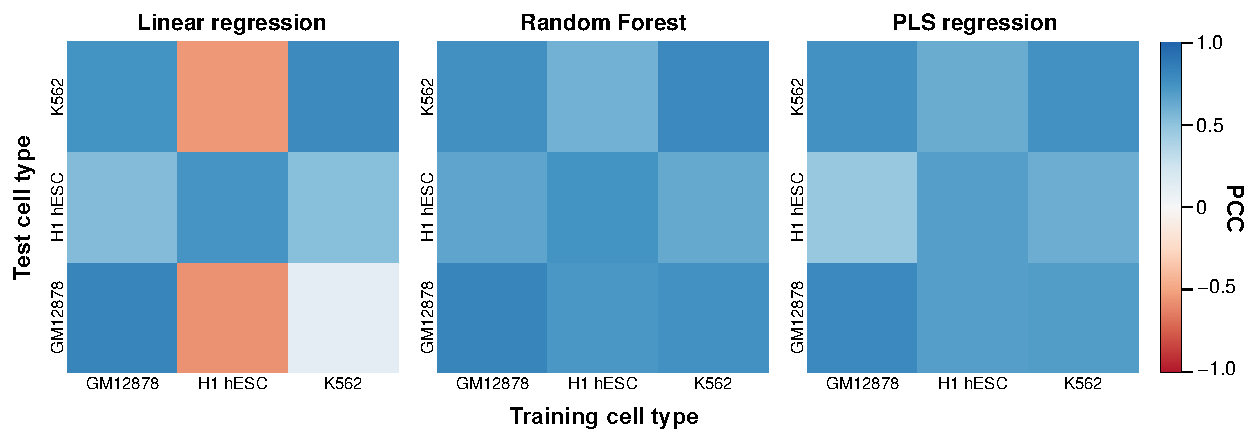
\includegraphics[width=1.2\textwidth]{figs/diffmethods.pdf}
\captionsetup{width=1.2\textwidth} 
\caption{ {\bf Comparison of Random Forest performance with other modelling approaches. }
Heatmaps show the Pearson correlation coefficient between predicted and observed compartment eigenvectors genome-wide for three regression techniques: multiple linear regression (LM), Random Forest (RF) and partial least squares (PLS). Results are summarised in Table \ref{tab:diffmethods}.
}\label{fig:diffmethods}
\end{center} 
\end{figure} 

Our results confirm RF as a suitable and powerful approach for modelling our relationships of interest in this work (Fig. \ref{fig:diffmethods}), with both the highest cell-type specific performance (PCC between predicted and observed $=0.790$) and on cross-applications (mean PCC $= 0.689$). 

Multiple linear regression assumes linear relationships between model parameters and input features and allows for simple, normally-distributed errors. Surprisingly, this simple approach is capable of accurate cell-type specific predictions (mean PCC $= 0.787$), likely due to the high raw correlation between the inputs and dependent variable. However this simple approach fails to cross-apply between cell types (mean PCC $=0.139$) indicating a problems with overfitting. This can be remedied through variable selection procedures, however a strength of the RF approach is that this step is not necessary, and pre-selection of model variables may result in a sub-optimal end result (ref XX).

Partial least squares regression is another technique which used dimensionality reduction to engineer a lower-dimension orthogonal feature set. Hence this method is well-suited to multi collinear inputs, such as our feature set. As expected, PLS regression provides highly accurate cell type specific predictions (mean PCC $=0.750) and during cross-application (mean PCC $=0.641), though in both cases produces slightly inferior results to RF models (Fig. \ref{fig:diffmethods}).

\begin{table}
\centering
\caption{ {\bf Performance comparison of different modelling techniques. }
 Comparison of mean Pearson correlation coefficient between predicted and observed compartment eigenvectors for three different modelling approaches: LM: linear regression; RF: Random Forest regression; PLS: partial least squares regression. Correlations were averaged per cell type over three cell types (cell type specific) and in the six possible crosses (cross-application) shown in Fig. \ref{fig:diffmethods}.
}
\label{tab:diffmethods}
\begin{tabular}{r|ccc}
& {\bf LM} & {\bf RF} & {\bf PLS} \\
\hline
Cell type specific  &  0.787 & 0.790 & 0.750 \\
Cross-application  & 0.139 & 0.689 & 0.641
\end{tabular}
\end{table}

\subsection{Non-independence}

% use n-1, n-2, ... as predictors for bin N

As recognised through our use of Hidden Markov Models (Methods XX), consecutive bins along a chromosome are non-independent yet thus far predictive models have not considered this inter-dependence. 

This is for two reasons: firstly non independence could be thought of as an artefact of bin-sizing (we have elected to use regular, fixed binning beneath the scale of compartments themselves whereas another approach could use variable bin sizes, for example per compartment, TAD or restriction fragment); secondly using information of a bin's surroundings may obscure by proxy the chromatin features which would otherwise prove predictive. As an example, knowing that bin $x_{i-1}$ and bin $x_{i+1}$ are in compartment state A would allow us with high confidence to predict the state of bin $x_i$, but without learning anything of any region's relationships with their histone modifications and bound factors.

\subsection{Correlating input features}\label{sec:corrinputs}

\ifstandalone
\begin{small}
\bibliography{/Users/benmoore/Documents/library,/Users/benmoore/Documents/customrefs}
\end{small}
\fi

\end{document}


\documentclass[a4paper,10pt,oneside]{book}

% packages 
\usepackage{arsclassica}    % fancy layout
\usepackage[english]{babel}\addto{\captionsenglish}{\renewcommand{\bibname}{References}}
\usepackage{caption}         % figure captions
\usepackage[square,numbers,super,sort&compress]{natbib}  % bibliography style
\usepackage[cc]{titlepic}    % enable logo on title page
\usepackage{graphicx}       % logo related

\usepackage{standalone}
\standalonetrue

% don't hang captions
\captionsetup{format=plain}

% bibliography
\bibliographystyle{../thesis}

% title setup
\title{ \vspace{3in} Unravelling higher order genome organisation {\small [working
    title]} \\ \vspace{2em} {\large {\bf Results 3: Domain boundaries}} }
\author{Benjamin L. Moore}
\titlepic{\vspace{2.2in} 
\includegraphics[width=\textwidth]{/Users/benmoore/hvl/1yrReport/figs/igmm.png}}

\begin{document}

%\maketitle

\chapter{Chromatin domain boundaries}

\section{Introduction}

Multiple studies have defined chromatin domains of different types, for example: chromosome compartments;\cite{Lieberman2009} topological associating domains (TADs);\cite{Dixon2012} contact and loop domains;\cite{Rao2014} physical domains;\cite{Sexton2012, Hou2012} and others.\cite{Filippova2014} The existence of these domains necessitates "boundary regions" either between consecutive domains or bookending more sparsely-positioned domains, however the functional relevance of said boundary regions is still open to debate.

In their study of topological domains, Dixon \emph{et al.} identified average enrichments over TAD boundary regions in both human and mouse for various features including CTCF and PolII.\cite{Dixon2012} Boundaries were also enriched for signs of active transcription, such as with the histone modification H3k36me3. These results, coupled with an observable enrichment for promoters at domain boundaries, have lead to the theory that boundaries may act as an additional layer of transcriptional control,\cite{Sexton2015} however an alternative theory could be that looping between enhancer elements and promoters results in an observable boundary through C-method experiments.\cite{Rao2014} Another non-exclusive explanation is that if chromatin domains represent co-regulatory regions as is widely thought,\cite{LeDily2014, Nora2013, Sexton2015} boundaries themselves could be mere side-effects and as such of limited biological interest.

An obvious experiment to resolve these opposing theories would be to delete a predicted boundary region and test for local changes in both contacts and expression. Such an experiment was performed on a region of the human X-chromosome containing the genes encoding the dosage-compensation long non-coding RNAs Xist and Tsix, which are separated by a TAD boundary.\cite{Nora2012} This study found that while histone modifications within the body of a TAD could be removed without affecting the structure, deletion of a boundary did have an effect and lead to increased intradomain contacts.\cite{Nora2012} Surpsingingly however, this effect was not total and some observable barrier remained, lending evidence that TADs may be centrally constrained, rather than by their borders.\cite{Nora2012} 

A second experiment used CRISPR genome editing to link TAD boundary changes with limb development disorders,\cite{Lupianez2015} indicating that boundary changes could provide an underlying explanation for pathogenic non-coding structural variants.\cite{Ren2015} Similarly, domain boundaries on X-chromosomes were found to be weakened following the disruption of condensation binding sites.\cite{Crane2015} Together these studies suggest a complex scenario whereby TAD boundaries are an important structural feature, yet do not fully explain domain partitioning.

Computational analysis of boundaries has emerged during the time this work was completed. Border "strength", here defined by the ratio of total intra:inter-domain contacts, was found to correlate with increased occupancy of a combination of bound architectural proteins.\cite{VanBortle2014}

Many questions remain about chromatin boundaries. For example, are the observed enrichments persistent across cell types and how do they compare across organisation strata, such as compartments and TADs? Through computational analysis of the set of boundaries re-called from published datasets, we can investigate these questions and probe boundary enrichments across a broad array of locus-level chromatin features.

\section{TAD and compartment boundaries}\label{sec:boundaryenrichments}

The mammalian genome is organized into TADs, predominantly self-interacting chromatin domains, with boundary regions reportedly associated with pronounced peaks and troughs of particular features within 500 kb of the predicted boundary.\cite{Dixon2012} Exploration of this phenomenon using a set of 24 mouse ESC chromatin features (and a smaller number of human ESC features) reportedly revealed enrichment peaks of CTCF, H3K4me3 and H3K36me3, as well as a pronounced dip in H3K9me3, suggesting that high levels of transcription may contribute to boundary formation.\cite{Dixon2012} However, it was unclear whether other features show unusual patterns in TAD boundary regions, and whether the constellation of features involved changes between cell types. The features associated with boundaries separating A and B compartments calculated from Hi-C eigenvectors have not been studied to our knowledge. The datasets assembled here, consisting of 35 matched chromatin features across three cell types, allow us to conduct the first comparative study of the constituents of human TAD and compartment boundary regions.

We derived TAD boundaries according to established methods (see Methods XX) for all three cell types under study. We then sought evidence for significantly enriched or depleted features at TAD boundary regions using a conservative approach (a nonparametric statistical test and Bonferroni multiple testing correction, see Methods XX).

\begin{figure}
\begin{center} 
\makebox[\textwidth][c]{ 
	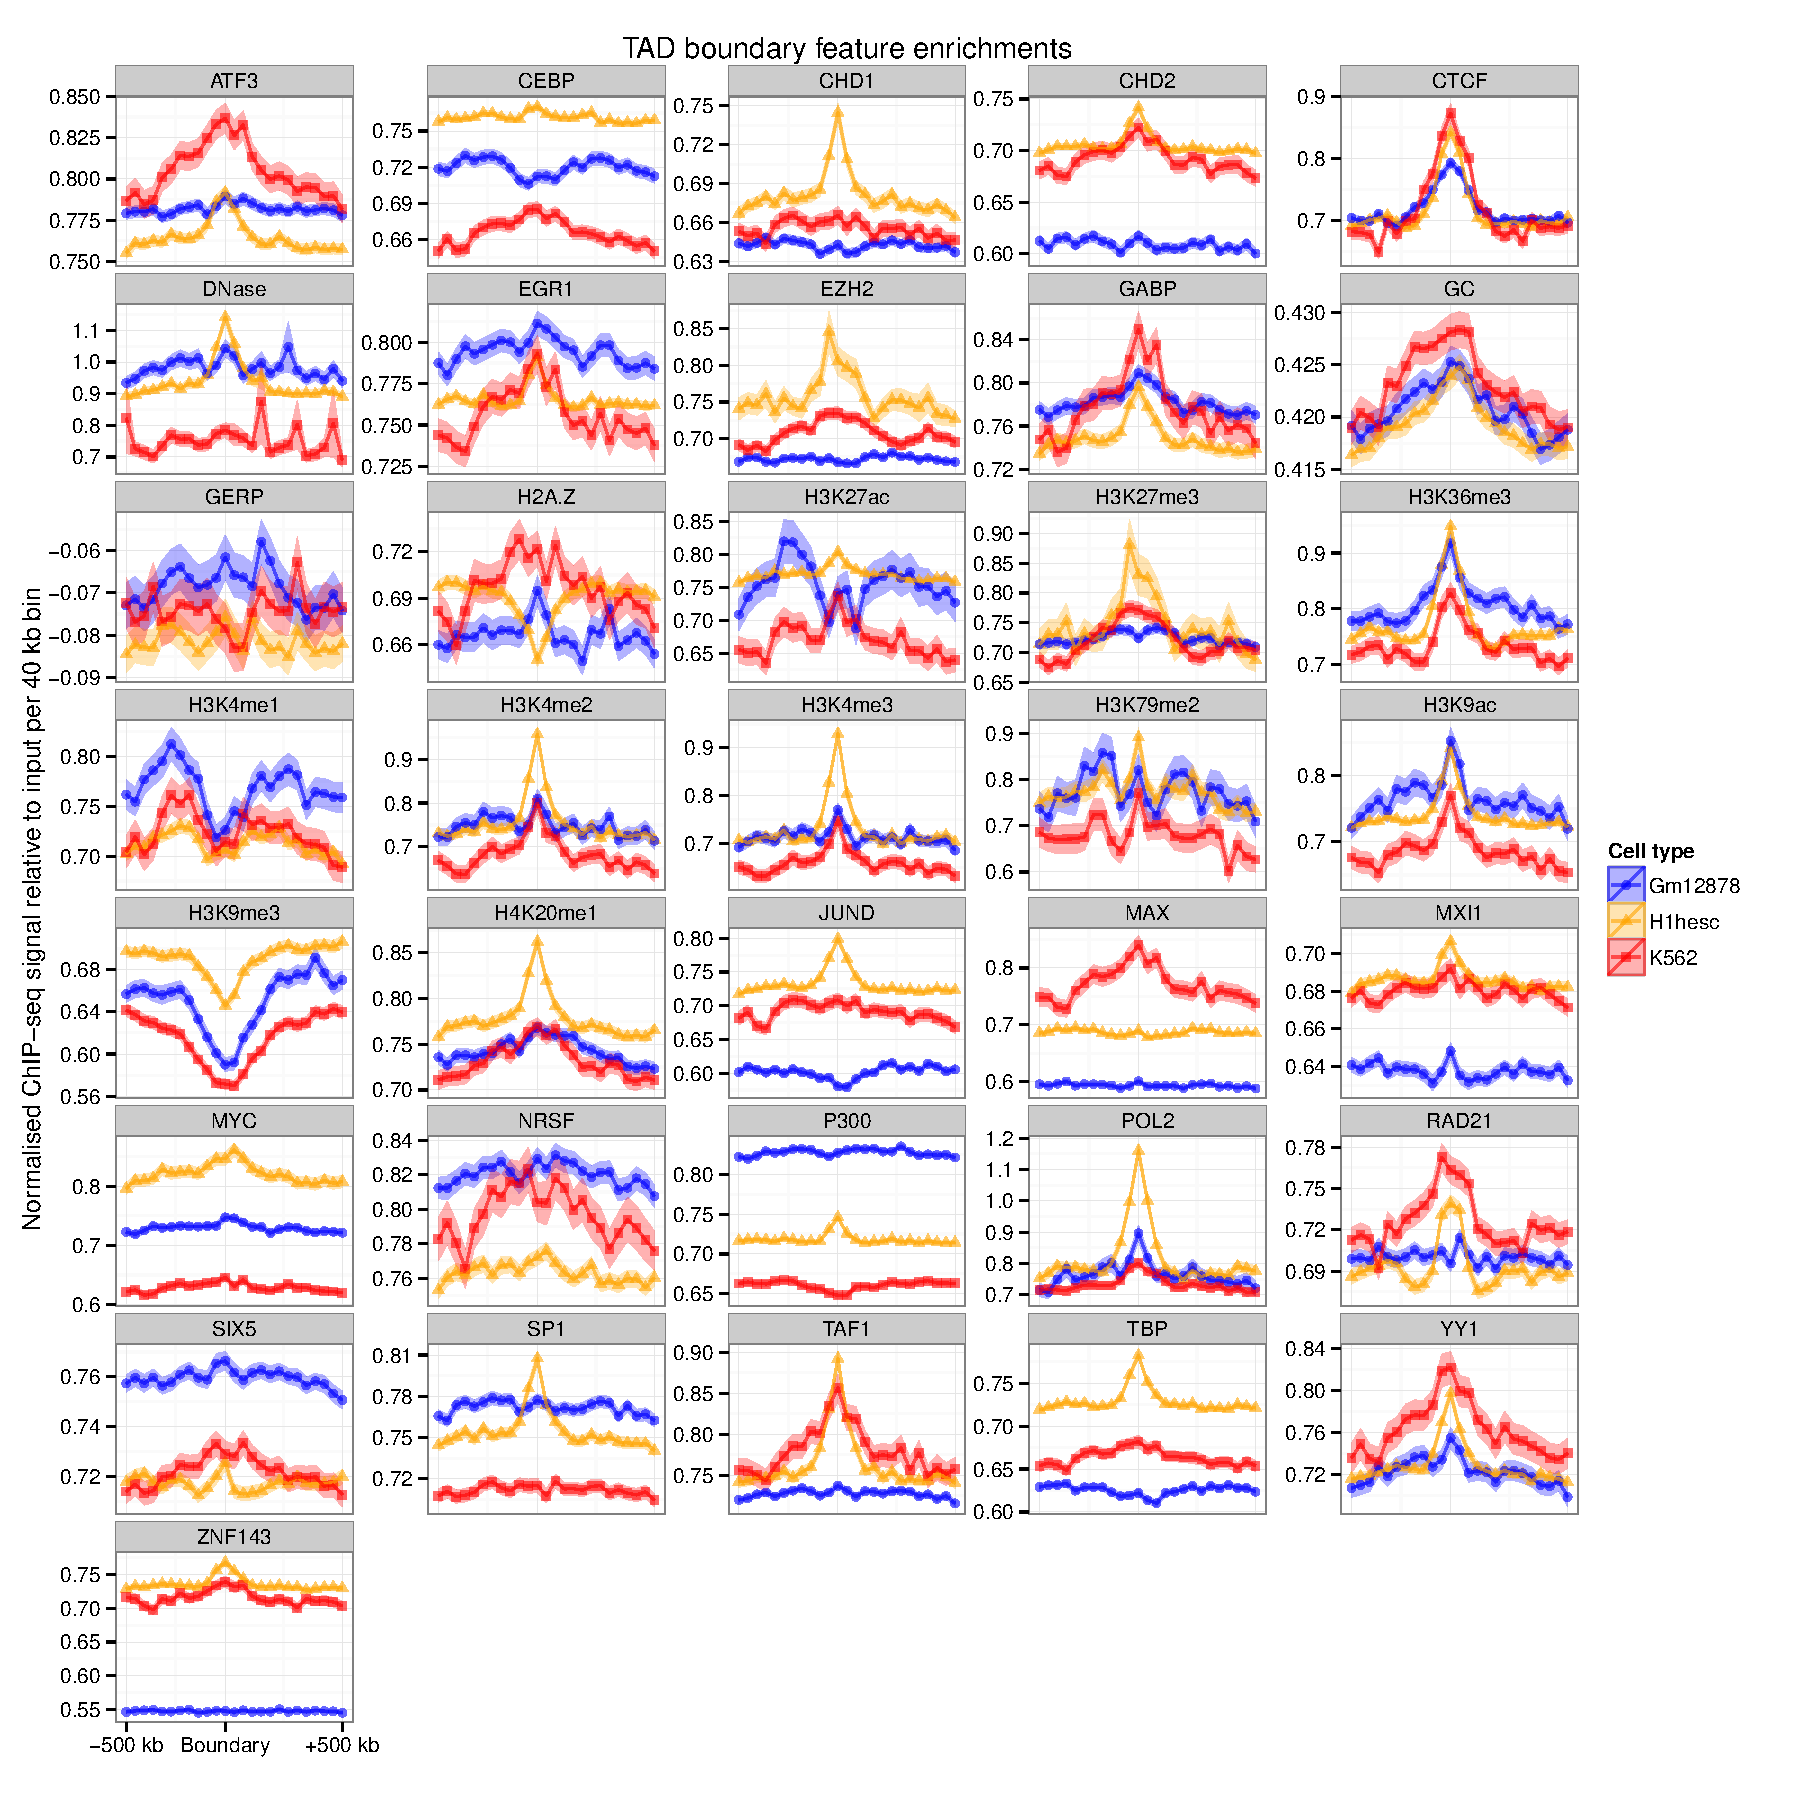
\includegraphics[width=1.2\textwidth]{figs/alltads.pdf}
}
\captionsetup{width=1.2\textwidth}
\caption[TAD boundary enrichments and depletions.]{ {\bf TAD boundary enrichments and depletions.}
36 features were averaged over 1 Mb windows centred on TAD boundaries genome-wide ($25 \times 40$ kb bins). Ribbons represent $95\%$ confidence intervals of the mean at each position.
}\label{fig:alltads}
\end{center}
\end{figure} 

\begin{figure}
\begin{center} 
\makebox[\textwidth][c]{ 
	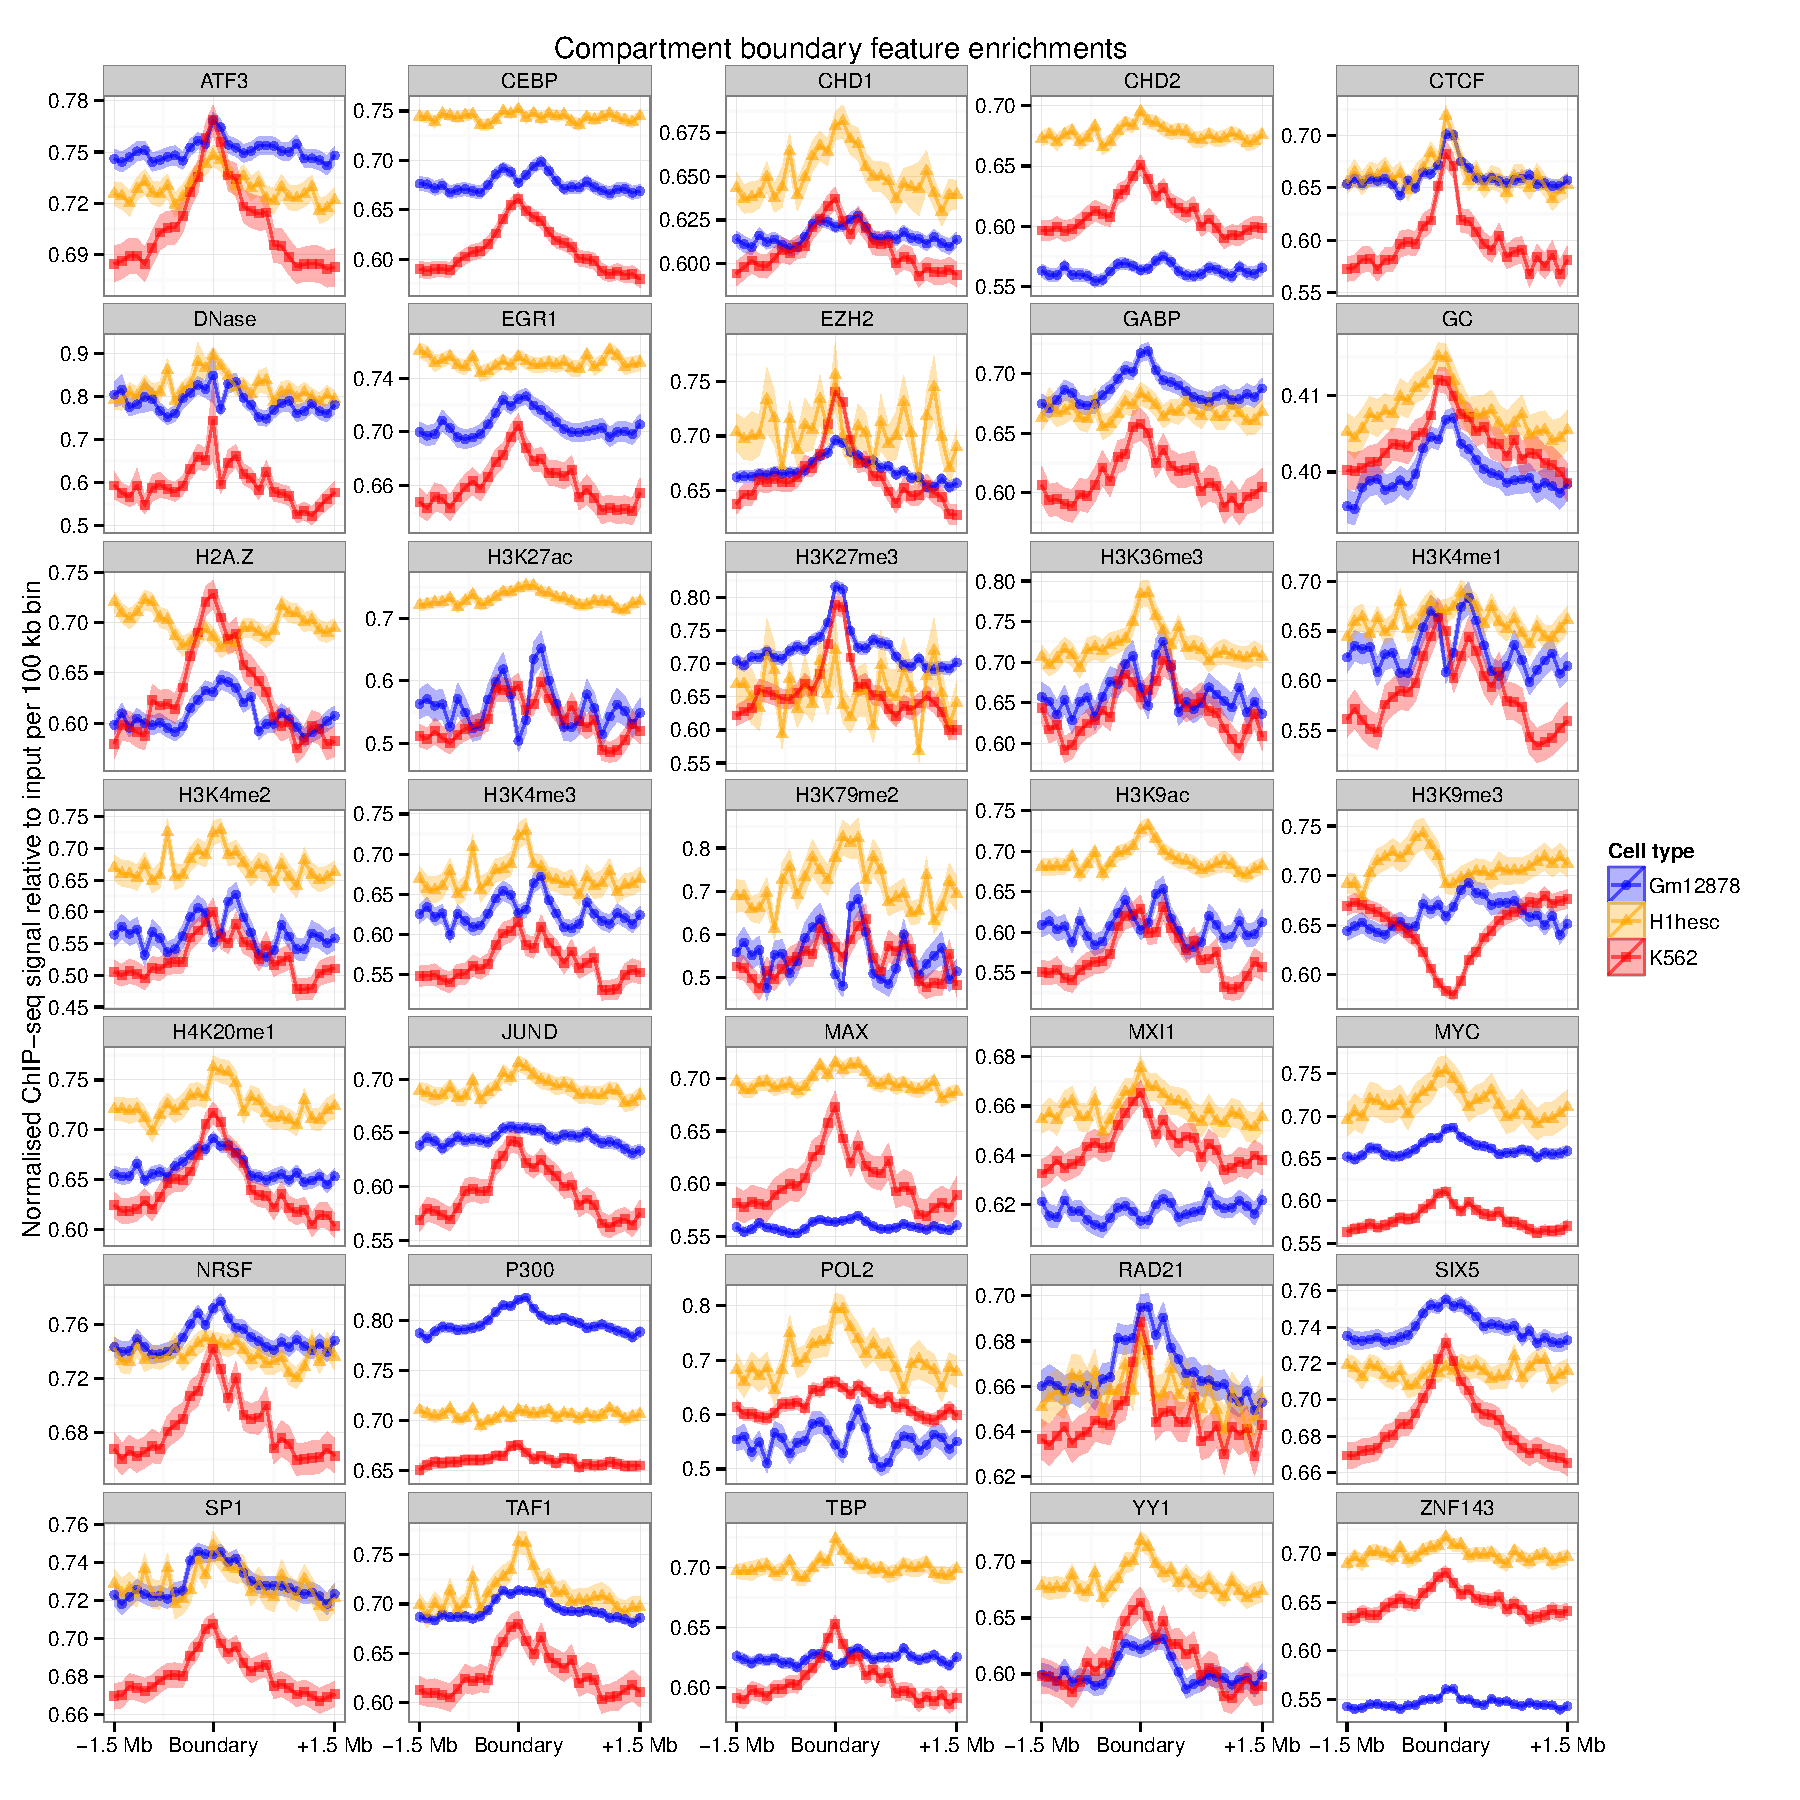
\includegraphics[width=1.2\textwidth]{figs/allcompartments.pdf}
}
\captionsetup{width=1.2\textwidth}
\caption[Compartment boundary enrichments and depletions.]{ {\bf Compartment boundary enrichments and depletions.}
36 features were averaged over 3 Mb windows centred on compartment boundaries genome-wide ($30 \times 100$ kb bins). Ribbons represent $95\%$ confidence intervals of the mean at each position.
}\label{fig:allcompartments}
\end{center}
\end{figure} 

Our findings confirmed the previously reported peaks (CTCF and POL2) and dip (H3K9me3) in ESC data, but also revealed substantial heterogeneity between cell types. CTCF binding was found enriched at TAD boundaries across all cell types, but other features, including H3K36me3 and H3K4me3, show dramatic peaks of enrichment in H1 hESC cells that are not seen consistently in other cell types (Figure 6, Additional file 1: Figure S12). Although the dip in H3K9me3 at TAD boundaries is seen in all cell types, the extent of the depletion varies and is weakest in H1 hESC cells. Many other features show significant, though often modest, enrichments in a particular cell type. However, overall the complexity of TAD boundaries (measured as the number of strongly enriched features) is notably higher in H1 hESC than in the other two, more differentiated, cell types (Figure 6), involving large increases in the binding of sequence specific factors such as SP1 and JUND.

\begin{figure}
\begin{center} 
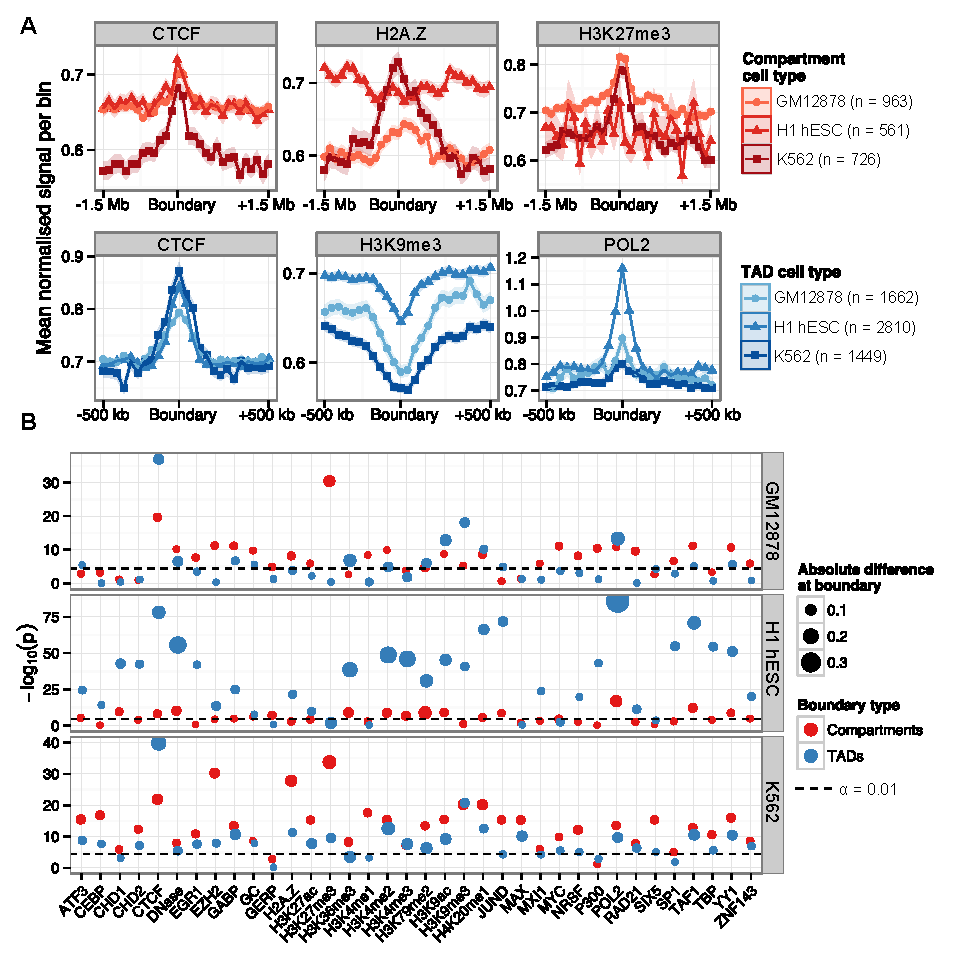
\includegraphics[width=\textwidth]{figs/boundarysummary.pdf}
\captionsetup{width=\textwidth}
\caption[Compartment and TAD boundary enrichment summary in three human cell types.]{ {\bf Compartment and TAD boundary enrichment summary in three human cell types.}
(A) Selected profiles for locus-level features are shown for TAD boundaries (CTCF, H3K9me3 and POL2) and compartment boundaries (H2A.Z, H3K4me2 and YY1), as a mean normalized ChIP-seq signal relative to input chromatin per bin ($\pm1$ standard error). TAD boundaries were examined over $40$ kb bins over the $1$ Mb flanking each boundary; compartment boundaries were examined over 100-kb bins over $3$ Mb. (B) The significance of enrichment or depletion ($-\log_{10}(p)$ two-tailed Mann--Whitney test) of a feature was calculated as the boundary bin relative to the ten most peripheral bins (five either side). Points are scaled by the absolute mean difference in signal over the boundary relative to the mean of peripheral bins. ChIP-seq, chromatin immunoprecipitation sequencing; TAD, topological domain.
}\label{fig:boundarysummary}
\end{center}
\end{figure} 

Across all three cell types several features demonstrate consistent
and statistically significant patterns at TAD boundaries (Figure 6,
Figure S12), including peaks associated with active transcription of
genes (POL2, H3K9ac) and dips in H3K9me3, as previously reported.\cite{Dixon2012} However other novel feature peaks of interest emerge
across cell types, such as peaks of H4K20me1, a modification
previously implicated in chromatin compaction.\cite{Evertts2013} We also observe consistent increases in GC content at TAD boundaries, at a scale that is difficult to reconcile with the presence of smaller-scale features such as repeat elements or CpG islands (Additional file 1: Figure S12).

Where neighbouring genomic regions occupy contrasting A and B nuclear
compartments, the disparity implies the presence of a boundary
region. Putative compartment boundaries were identified by using an
HMM to infer the state sequence of A/B compartments across the genome
based on observed principal component eigenvectors. Analogously to the
TAD boundary analysis we then sought significant enrichments or
depletions in 36 chromatin features over these compartment boundaries
(Figure 6, Figure S13).  Compartment boundaries display similar
spectra of enrichments to previously studied TAD boundaries
\cite{Dixon2012} but at lower resolution, reflecting the different
scales of these levels of organization (Figure 6B, Figure S13). Peaks
associated with active promoters (POL2, TAF1, H3K9ac) are again
evident. Parallel enrichments of CTCF, YY1 and H4K20me1 are also seen
at compartment boundaries, as they were for TAD boundaries, in each
cell type under study. In addition, compartment boundaries show
enrichments of H3K79me2, which is known to play critical roles in
cellular reprogramming.\cite{Onder2012} Remarkably, H3K79me2 has
also recently been shown to mark the borders of small (hundreds of bp)
regions of open chromatin.\cite{Chai2013} Thus there may be
similarities in chromatin compaction boundaries at very different
scales.

Certain features show intriguing contrasts between cell types the
histone variant H2A.Z lacks any trace of enrichment at H1 hESC
compartment boundaries, but is significantly enriched in the other two
cell types (Figure 6A), consistent with reports describing H2A.Z
relocation during cellular differentiation.\cite{Ku2012} Compartment
boundaries also show enrichment for the cohesin complex subunit RAD21
in the two hematopoietic cell types , and cohesin is
another factor implicated in modulating nuclear architecture in
partnership with CTCF.\cite{Zuin2013} Various other enrichments
with very modest effect sizes are also evident at compartment
boundaries (Figure 6B, Figure S13). In contrast to TAD boundaries, the
composition of compartment boundaries appears least complex in H1
hESC, relative to the other two cell types. Overall compartment and
TAD boundaries are associated with overlapping spectra of chromatin
features across cell types. These involve DNA binding proteins
implicated in chromosome architecture (CTCF, YY1, RAD21), but also
implicate the initiation and repression of transcription as critical
to boundary formation. However these two boundary classes occur at
different scales, with patterns of informative features typically
spanning regions up to 500 Kb for TAD boundaries, and patterns
associated with compartment boundaries often spanning more than 1 Mb.

\subsection{CTCF and YY1}

\begin{figure}
\begin{center} 
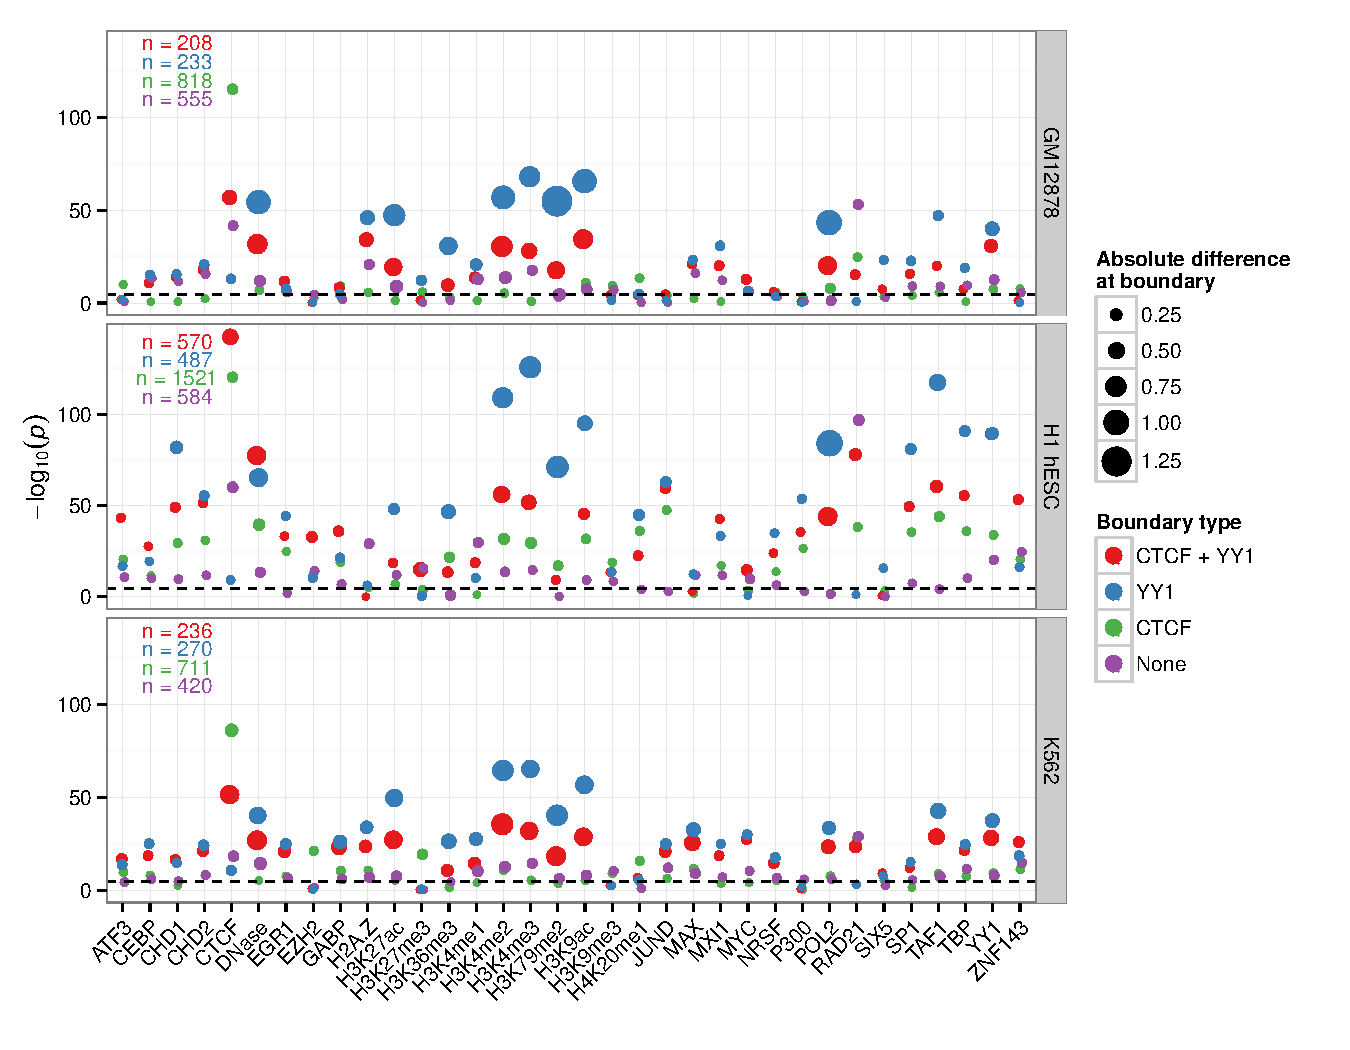
\includegraphics[width=1.2\textwidth]{figs/ctcfyy1.pdf}
\captionsetup{width=\textwidth}
\caption[Distinct enrichments of CTCF and YY1 boundaries.]{ {\bf Distinct enrichments of CTCF and YY1 boundaries.}
TAD boundary feature enrichments are shown (as in Fig. \ref{fig:boundarysummary}) for boundaries
split into classes based on specific enrichments: CTCF and YY1 groups are
those boundaries with at least one ENCODE region peak\cite{Dunham2012} for
their respective features, while CTCF + YY1 is the group of boundaries which had one or more
overlapping peaks for these two factors. Boundaries in the �none� group has neither
a CTCF or YY1 region peak called (but can still
be enriched for their respective features in terms of raw signal). 
}\label{fig:ctcfyy1}
\end{center}
\end{figure} 

Significant peaks in YY1 are evident in all cell
types, which is intriguing given the evidence that YY1 and CTCF
cooperate to affect long distance interactions.\cite{Atchison2014} Co-binding of CTCF with YY1 has also been shown
to identify a subset of highly conserved CTCF sites.\cite{Schwalie2013} Co-binding of CTCF and YY1 may also therefore be
a contributing factor in the establishment of TAD boundaries, which
appear to be broadly conserved across mammals.\cite{Dixon2012} To
test this, we split our sets of TAD boundaries into those possessing
ChiP-seq peaks (region peaks called by ENCODE \cite{Dunham2012}) for
CTCF, YY1, both CTCF and YY1 (overlapping peaks) and neither. We then
tested each boundary subset for genome-wide enrichments of the other
features in our dataset (Figure S14). Unexpectedly, we found that
boundaries marked by YY1 (without overlapping CTCF peaks) were
generally most strongly-enriched for other features in our dataset. We
also found that boundaries lacking both CTCF and YY1 peaks showed
instead the strongest enrichments for RAD21 in each cell type (Figure
S14), reinforcing previous findings that describe the distinct
influences of CTCF and cohesin in organizing chromatin structure.\cite{Zuin2013, Seitan2013, Phillips-Cremins2013}

% Schwalie: These observations suggest that with respect to transcriptional activity, YY1 is the functionally dominant factor at co-bound locations.

\subsection{Repeats}\label{sec:repeats}

Dixon \emph{et al}.'s study of TAD boundaries identified short interspersed element (SINE) repeats as being enriched over domain boundaries and suggested roles for these repeats in altering genome organisation, in line with prior evidence.\cite{Dixon2012, Lunyak2007} Interestingly, SINE elements are thought to be responsible for spreading CTCF binding sites through mammalian genomes\cite{Schmidt2012} (thought not in primates\cite{Schwalie2013}). Analysis of recent high-resolution Hi-C data again reported a SINE B2 link with CTCF loops in mice.\cite{Rao2014} Together these results suggest repeats could be a key component in the makeup of domain boundaries.

To investigate this, we used the \texttt{RepeatMasker}\cite{Tarailo-Graovac2009} software package to call repeat classes and families in the \texttt{hg19} and \texttt{mm10} genome assemblies. Counts for each annotated feature were then average over boundaries as described previously (Methods XX).

\begin{figure}
\begin{center} 
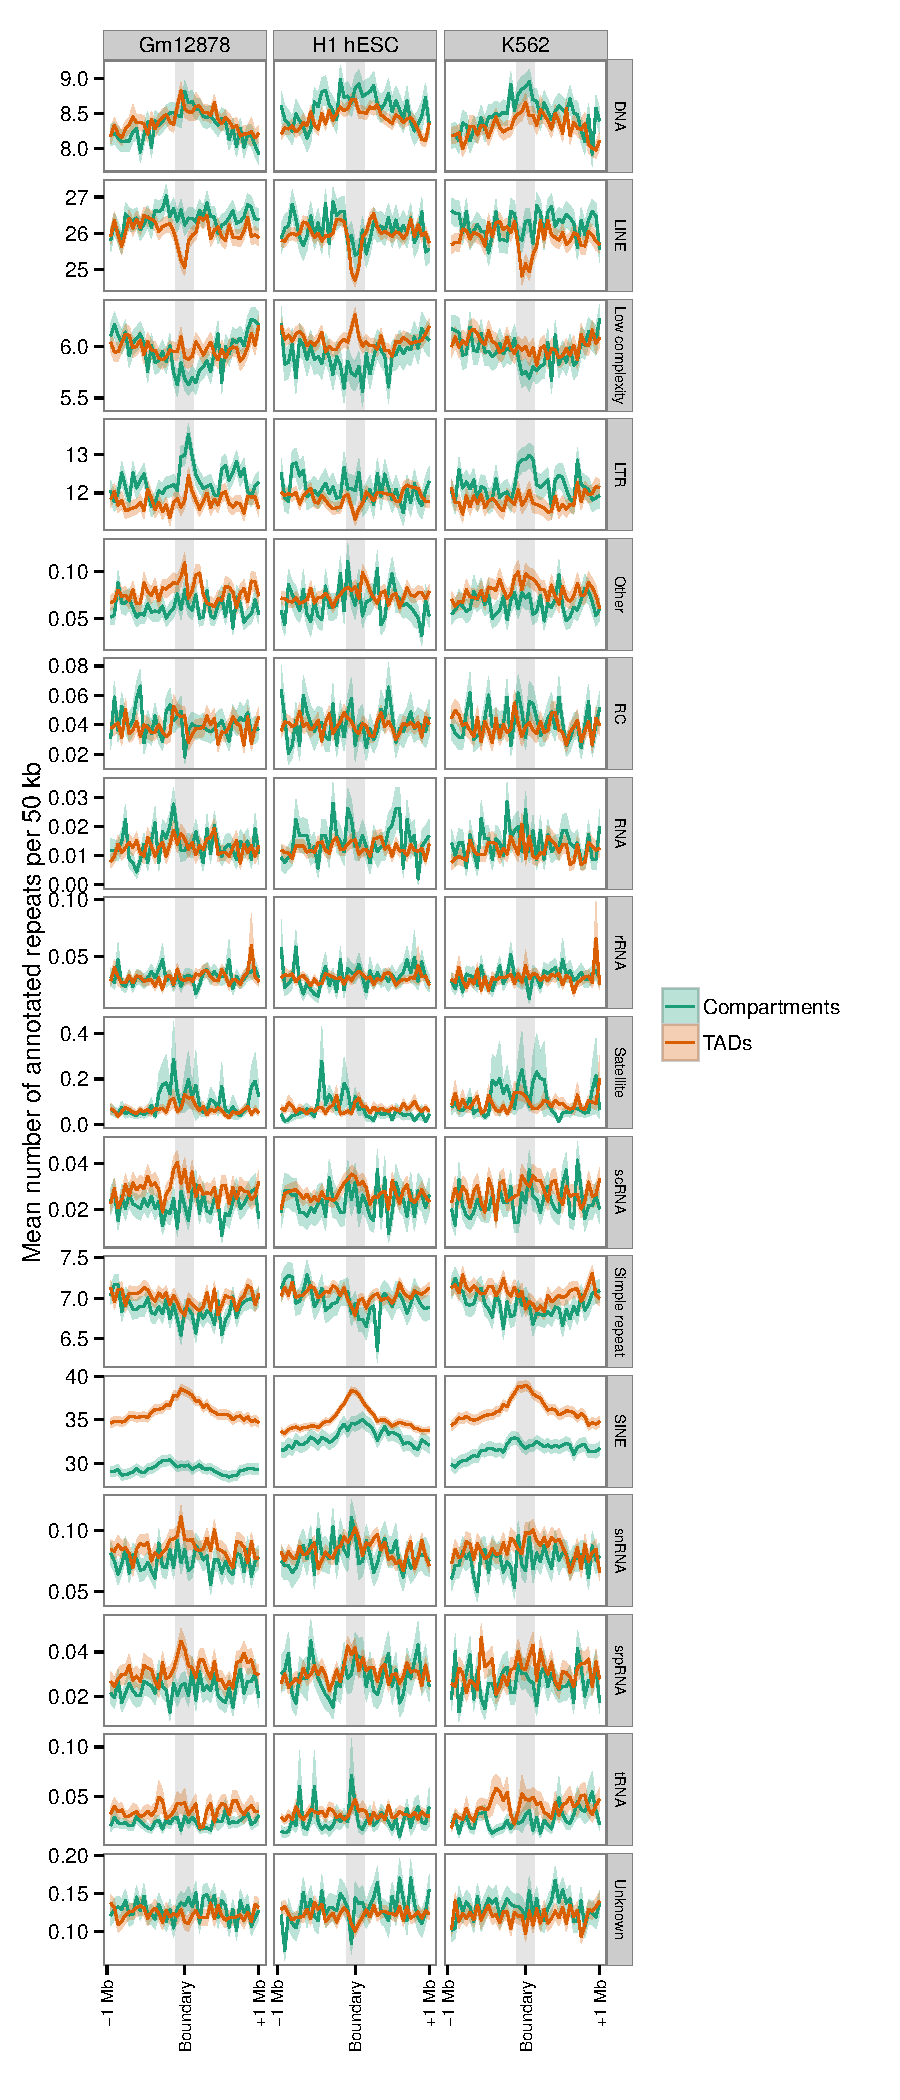
\includegraphics[width=.88\textwidth]{figs/rep_classprofiles.pdf}
\captionsetup{width=\textwidth}
\caption[Repeat class average-o-grams over all TAD and compartment boundaries.]{ {\bf Repeat class average-o-grams over all TAD and compartment boundaries.}
RepeatMasker repeat annotations are counted per 50 kb for 1 Mb either side of each TAD and compartment boundaries. The mean count genome-wide is plotted with $\pm 95\%$ confidence intervals.
}\label{fig:rep_classprofiles}
\end{center}
\end{figure} 

At the level of repeat class, we corroborate the findings of \citet{Dixon2012} that the majority of repeat classes show no enrichment or depletion at TAD boundaries, and we find that this also holds for compartment boundaries (Fig. \ref{fig:rep_classprofiles}). A notable exception is the short interspersed element (SINE) repeat class which appears to be enriched at TAD boundaries in each cell type. Testing the significance of this observed peak confirms this to be the case, with SINEs significantly enriched at TAD boundaries in each cell type, and borderline significant enrichments can also be observed at compartment boundaries (Fig. \ref{fig:rep_classbubble}).

\begin{figure}
\begin{center} 
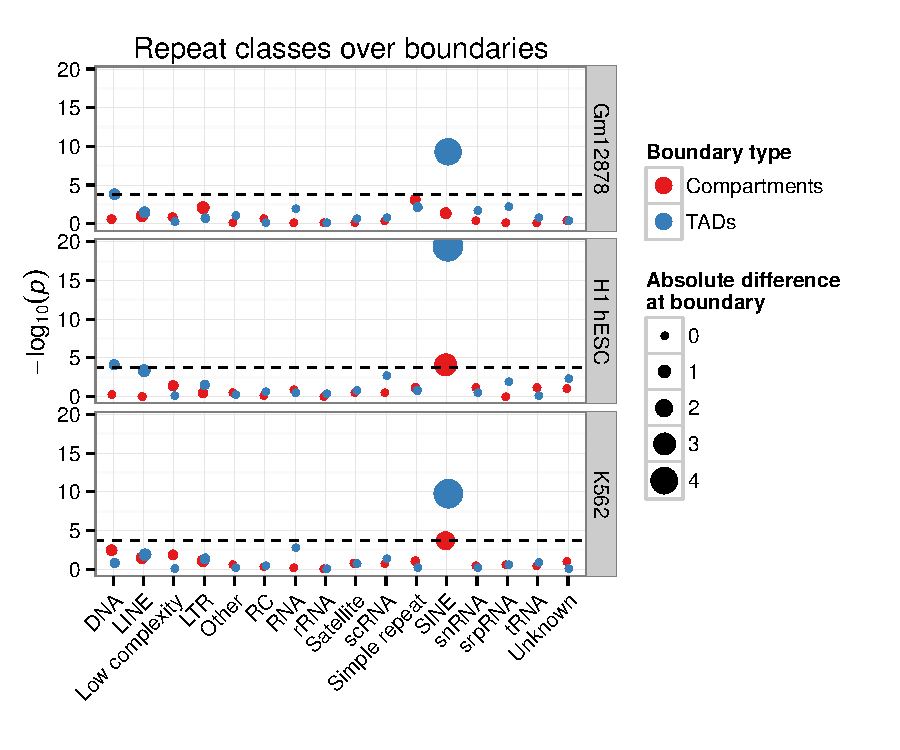
\includegraphics[width=.9\textwidth]{figs/rep_classbubble.pdf}
\captionsetup{width=\textwidth}
\caption[Significance and effect sizes of repeat class enrichments/depletions over boundaries.]{ {\bf Significance and effect sizes of repeat class enrichments/depletions over boundaries.}
Boundary profiles (Fig. \ref{fig:rep_classprofiles}) were tested for enrichment or depletion of each factor at the boundary bin relative to peripheral non-boundary bins (see Methods XX). Bubble area is proportional to the raw effect size of an enrichment or depletion. The Bonferroni-corrected significance threshold is highlighted with a dashed line.
}\label{fig:rep_classbubble}
\end{center}
\end{figure} 

Repeat class profiles also suggest LINEs may be depleted over TAD boundaries and DNA repeats may be enriched at both boundary types (Fig. \ref{fig:rep_classprofiles}), however statistically these observations do not surpass our pre-defined significance threshold ($\alpha = 0.05$) after multiple testing correction (Fig. \ref{fig:rep_classbubble}).

Repeat classes can be broken into smaller repeat families. \citet{Dixon2012} reported that the Alu (or B1 in mouse) repeat families are enriched over TAD boundaries. Again we can reproduce this finding and extend it to compartment boundaries (Fig. \ref{fig:rep_fambubble}). 

\begin{figure}
\begin{center} 
\makebox[\textwidth][c]{ 
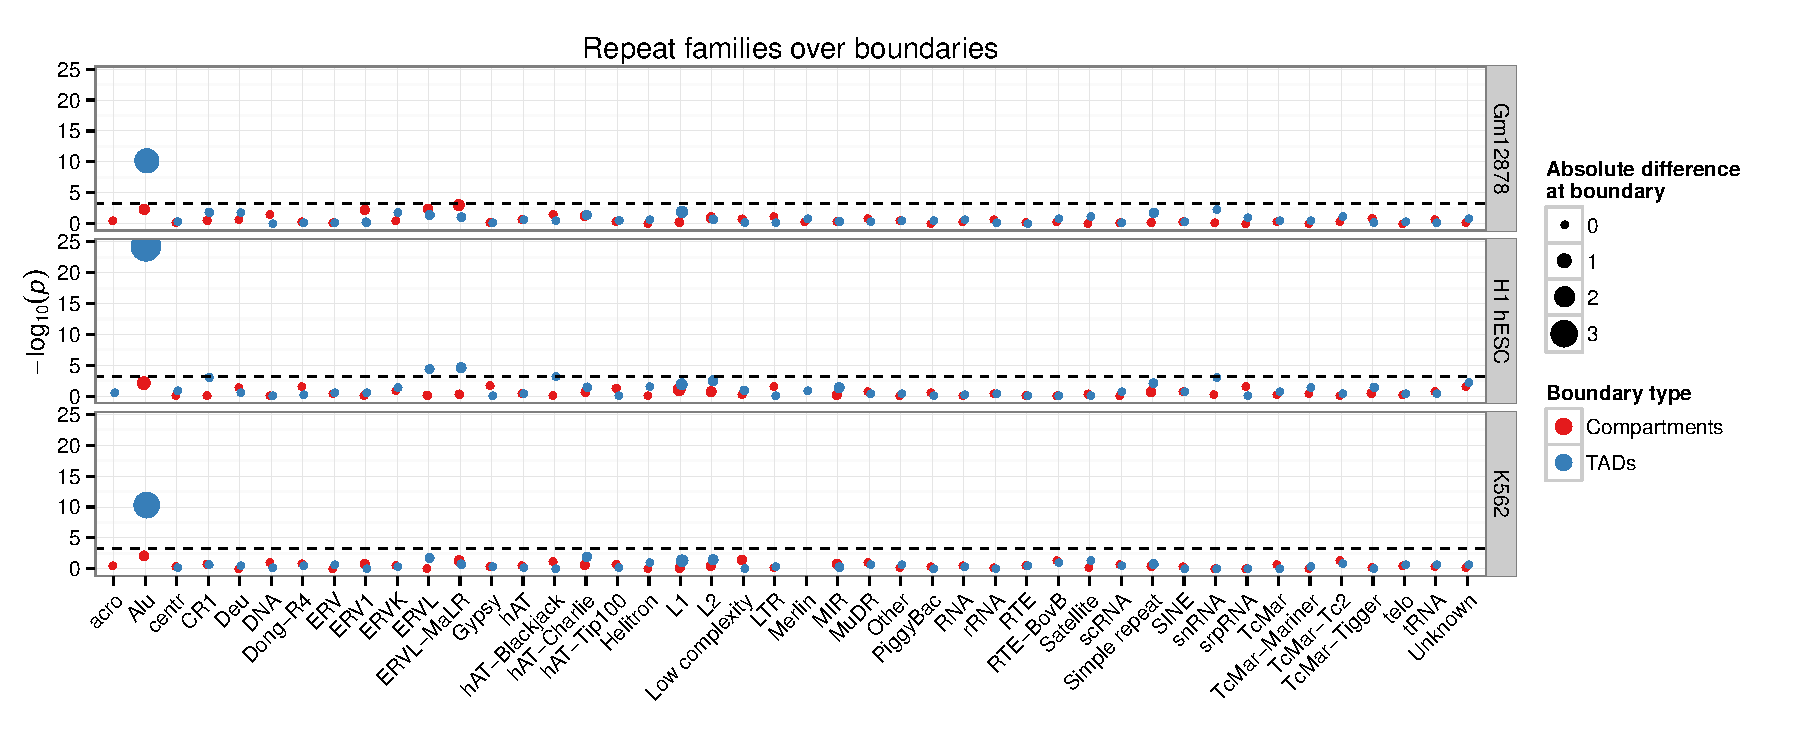
\includegraphics[width=1.6\textwidth]{figs/rep_fambubble.pdf}
}
\captionsetup{width=\textwidth}
\caption[Significance and effect sizes of repeat family enrichments/depletions over boundaries.]{ {\bf Significance and effect sizes of repeat family enrichments/depletions over boundaries.}
As per Fig. \ref{fig:rep_classbubble} but for a higher resolution repeat classification.
}\label{fig:rep_fambubble}
\end{center}
\end{figure} 

% Figure: profiles of those significant + suggestive from all repeat family profiles

\section{De novo boundary prediction}

We have shown TAD and compartment domain boundaries to be well-marked by a variety of features. Compartment boundaries are successfully predicted as a side-effect of modelling the continuous compartment profile eigenvector (Section XX) however a related measure of activity and repression does not exist for TADs.

We attempted to model TAD boundaries in a variety of ways: firstly a using a class-balanced classification framework and secondly through indirect models of directionality index and the downstream domain-caller HMM state.\cite{Dixon2012}

\section{MetaTAD boundaries}\label{sec:metatads}

\begin{figure}
\begin{center} 
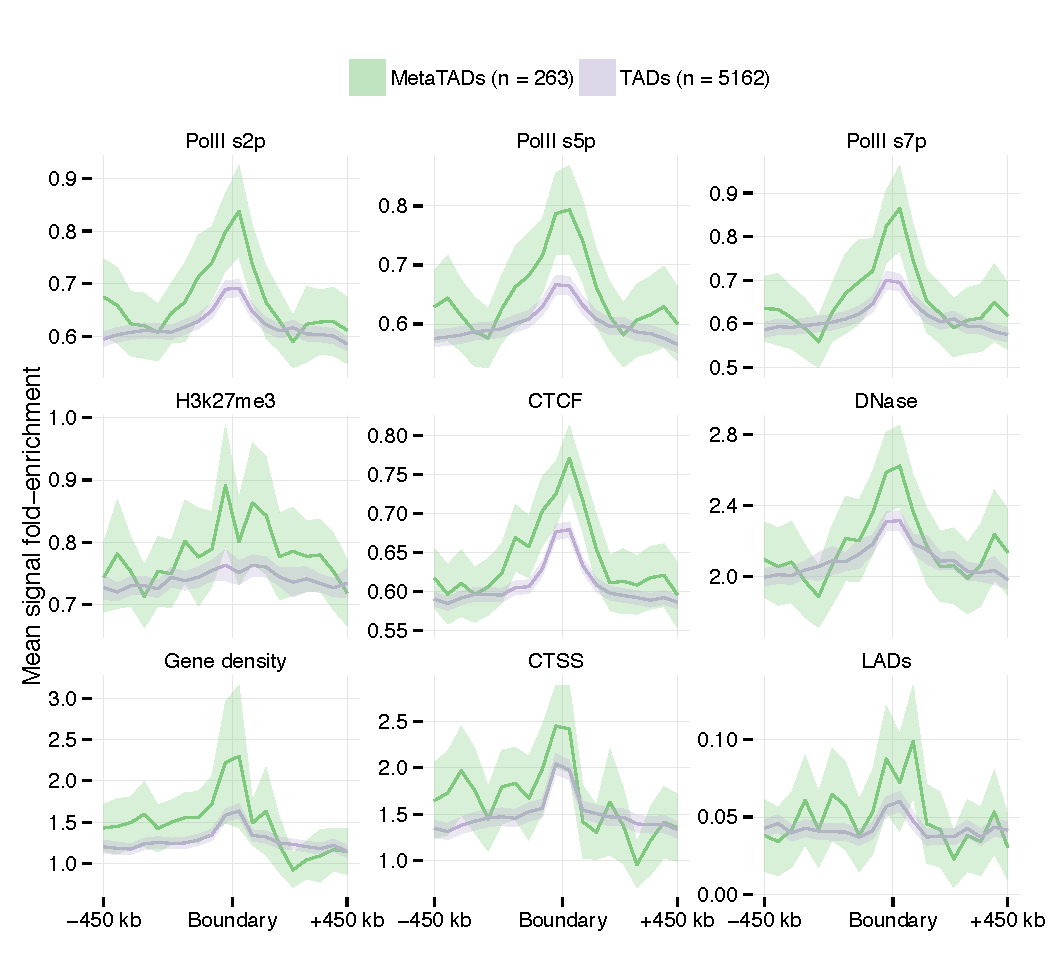
\includegraphics[width=.9\textwidth]{figs/mt_feats.pdf}
\captionsetup{width=\textwidth}
\caption[Large metaTADs show greater enrichments for an array of boundary features.]{ {\bf Large metaTADs show greater enrichments for an array of boundary features.}
Genome-wide profiles of epigenomic features and gene densities averaged over all TAD and metaTAD (10 -- 40 Mb) boundaries (ribbons show $95\%$ confidence intervals of the mean).
}\label{fig:mtfeats}
\end{center}
\end{figure} 

Our collaborators uncovered the concept of "metaTADs": sequential aggregations of adjacent and strongly-interacting TADs to form a hierarchy of domain organisation covering each chromosome.

MetaTADs are constructed simply by performing constrained heretical clustering based on inter-TAD contacts. That is, those two neighbour TADs that have the largest number of interTAD contacts are linked to form a metaTAD and this process is recursed until all TADs on a chromosome are joined into a tree-like network which fully describes the hierarchical nature of domain organisation.

My contribution to this work was to explore these newly-described metaTAD structures and perform boundary analysis as was done with TADs and compartments (Section \ref{sec:boundaryenrichments}). A hypothesis to test could be that boundaries of larger metaTAD structures could display greater enrichments for boundary-defining features.

\subsection{Lamin associated domains}

\begin{figure}
\begin{center} 
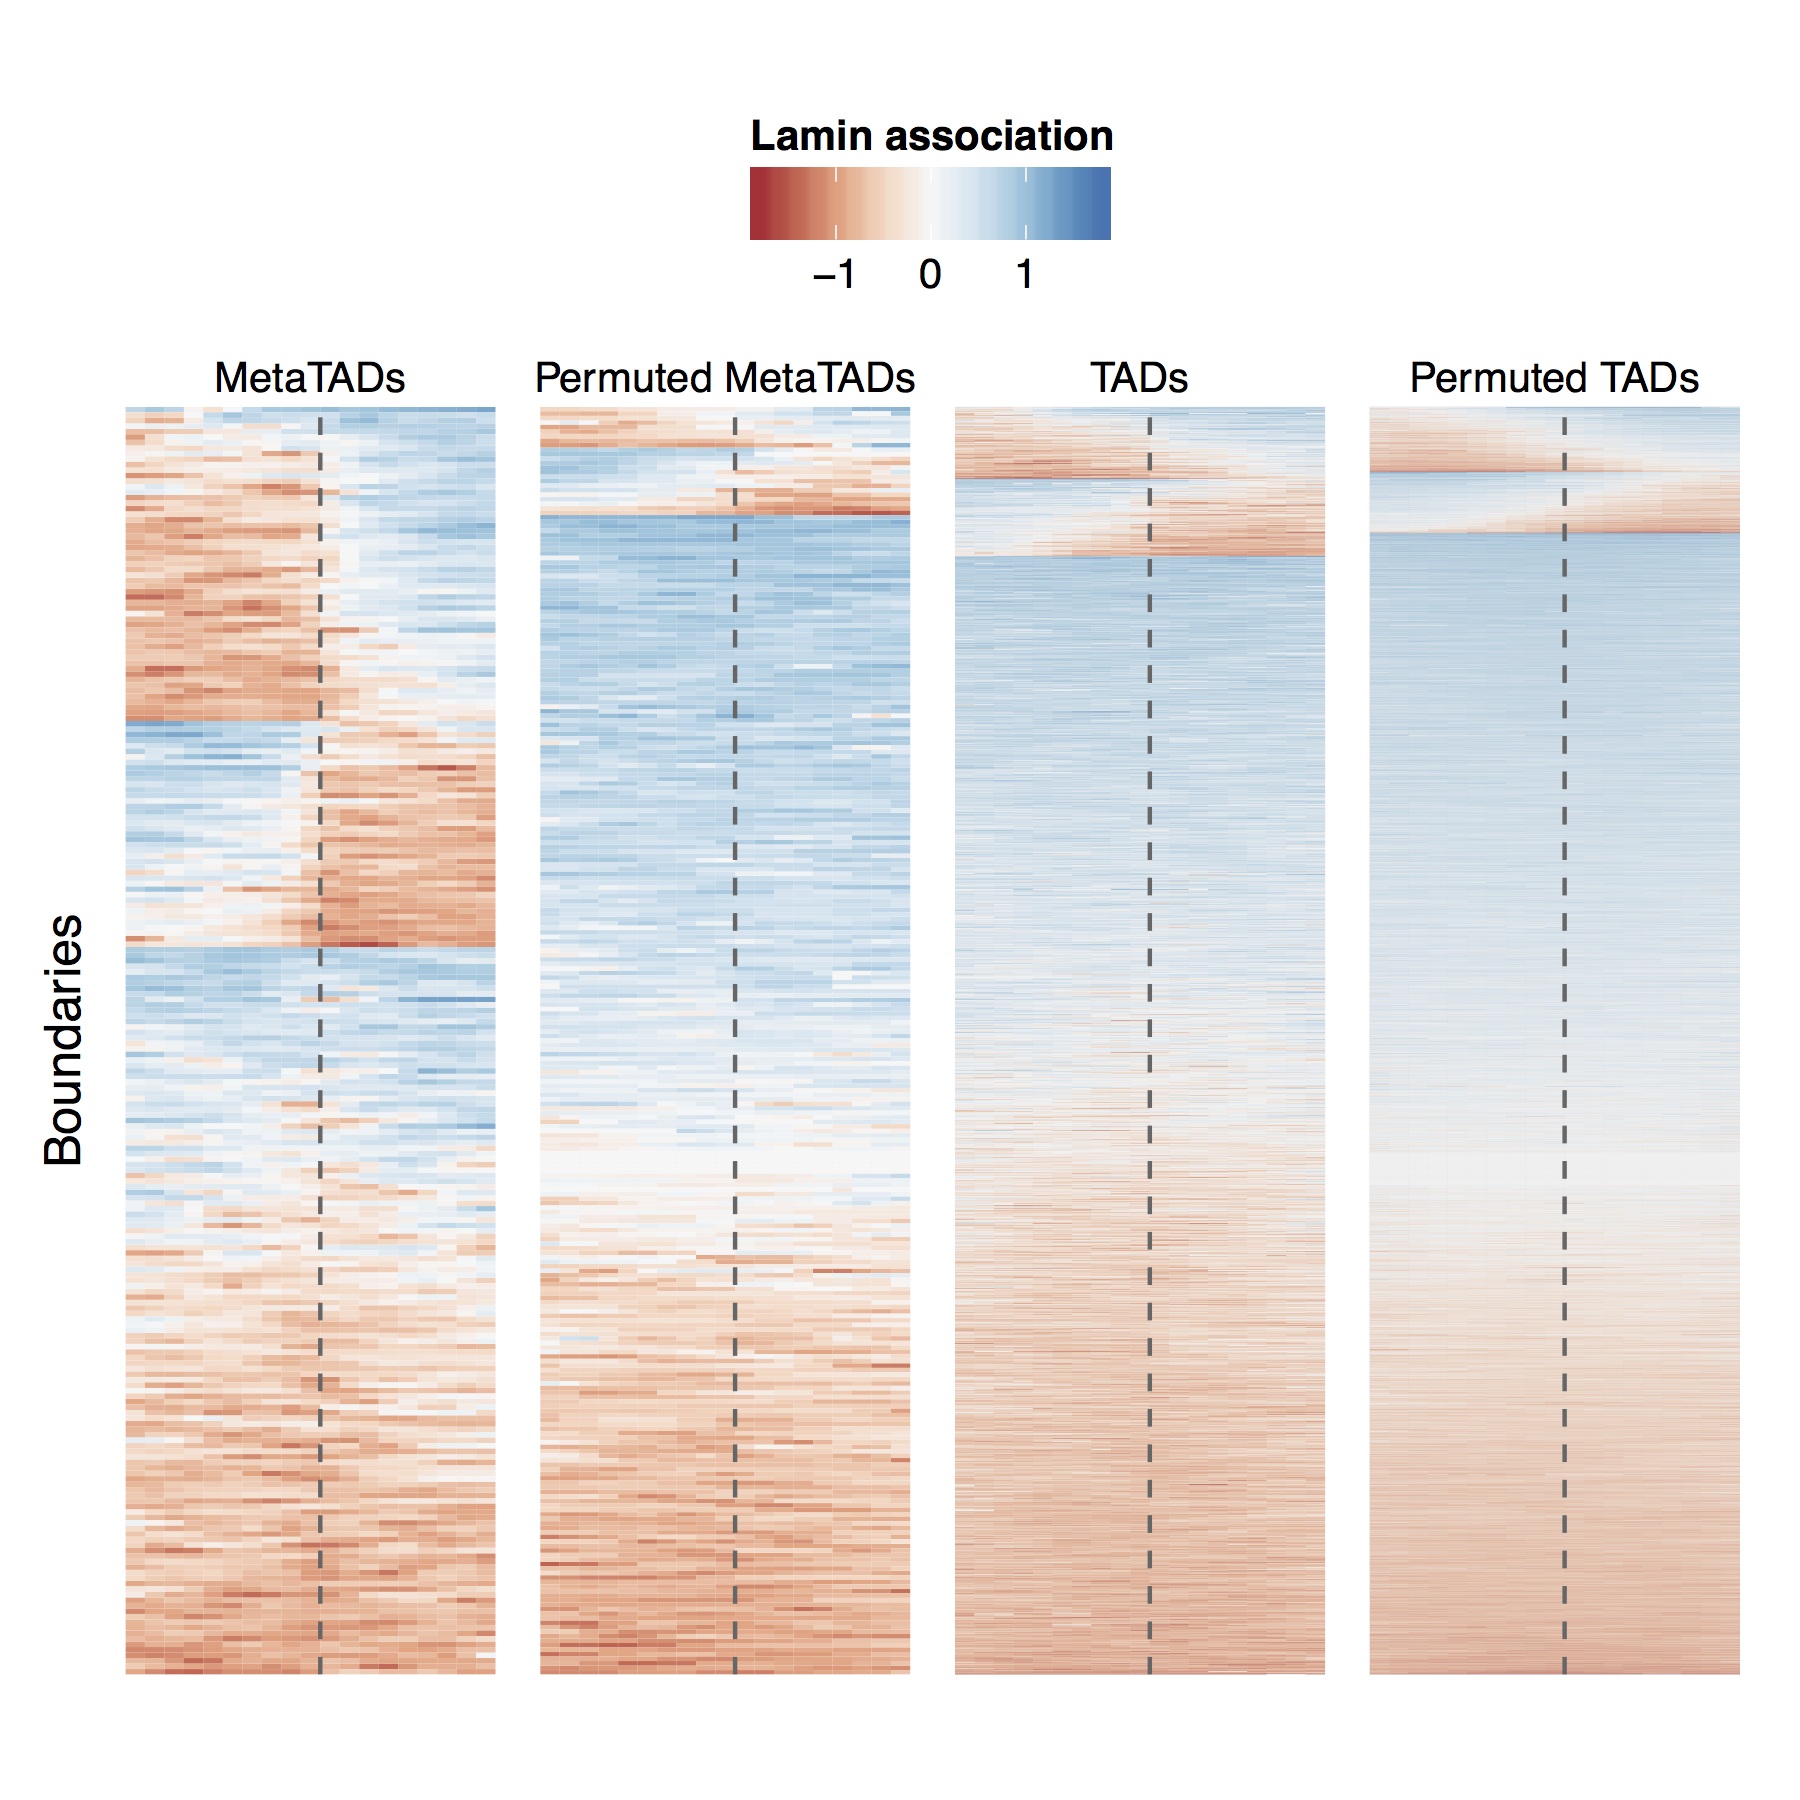
\includegraphics[width=.9\textwidth]{figs/mt_laminperm.png}
\captionsetup{width=\textwidth}
\caption[MetaTADs align with lain associated domains.]{ {\bf MetaTADs align with lain associated domains.}
Heatmaps of LaminB1 association microarray probe intensity values over MetaTAD boundaries (from domains of size 10 -- 40 Mb) and TAD boundaries, are displayed alongside examples of circularly-permuted boundaries. $42.6\%$ of MetaTAD boundaries (10 -- 40 Mb) had an absolute linear regression coefficient $>.05$ of lamin association intensities, indicating a boundary transition (versus $15.8\%$ expectation from 1000 circular permutations, $p < 1 \times 10^{-4}$). TAD boundaries were also significantly more associated with lamin association transitions (Observed: $11.8\%$, Expected: $9.5\%$; empirical p-value: $p < 1 \times 10^{-4}$). Profiles are shown $\pm450$ kb from each boundary.
}\label{fig:mtlamin}
\end{center}
\end{figure} 

\subsection{Boundaries over a time series}

\begin{figure}
\begin{center} 
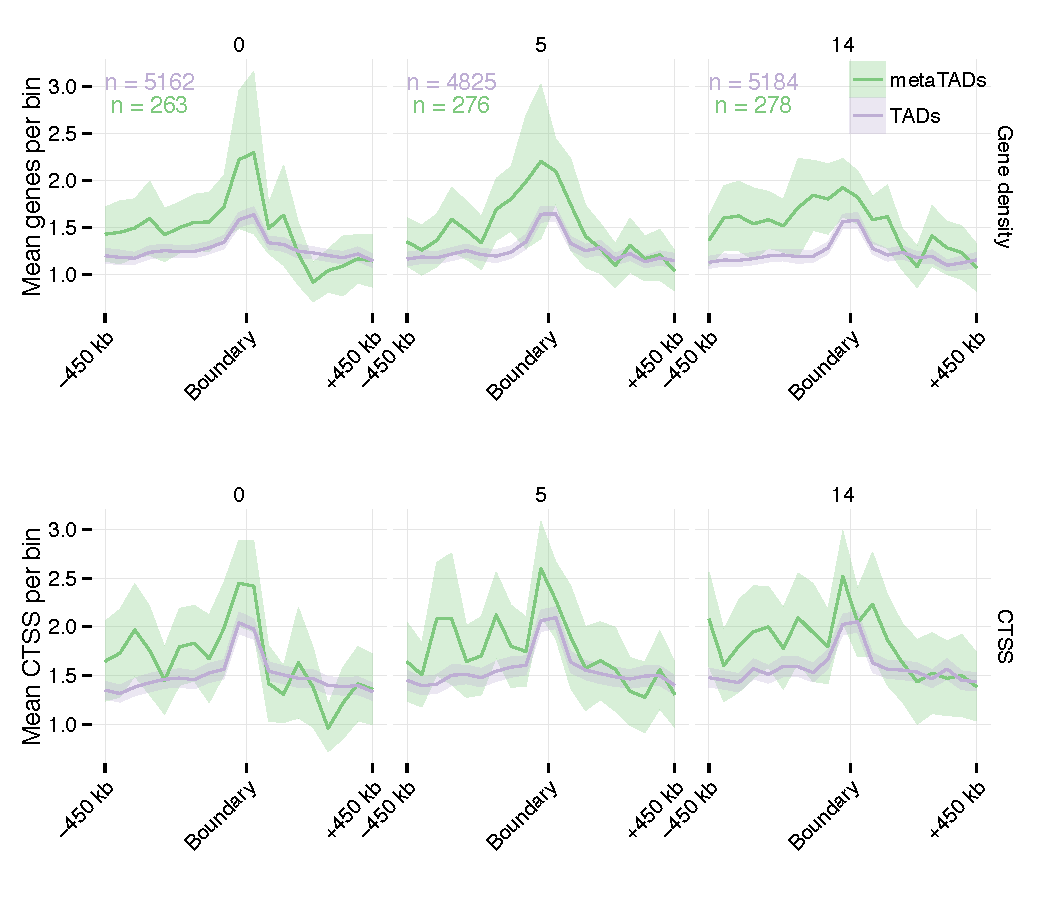
\includegraphics[width=.9\textwidth]{figs/mt_ts.pdf}
\captionsetup{width=\textwidth}
\caption[Observed enrichments persist over a time series.]{ {\bf Observed enrichments persist over a time series.}
CAGE-defined active TSS (CTSS) were counted per 50 kb bin across each TAD and MetaTAD (10 -- 40 Mb) boundary and averaged (ribbons show $95\%$ confidence intervals of the mean). Gene densities refer to mean counts of annotated genes per bin, with an overlap of at least 250 bp. Peak heights suggest modestly stronger enrichments at MetaTAD boundaries relative to TAD boundaries. 
}\label{fig:mtts}
\end{center}
\end{figure} 

\section{Other boundaries}

\subsection{Giemsa bands}

% text (colin's?) from pre-submission old manuscript draft
A recent analysis of Hi-C datasets examined the hierarchy of nuclear compartment and TAD organisation in human HeLa cells across the cell cycle. They found that interphase and metaphase chromatin structure are highly distinct, such that the TADs and compartments observed here are effectively abolished in metaphase.\cite{Naumova2013} This raises the question of how the structural organization seen in (and often shared between) interphase cells is inherited through the cell cycle.

Human Giemsa metaphase banding (G-band) pattern data have been integrated with the human genome assembly, and although such data are widely used, they are also necessarily of low resolution.\cite{Furey2003} These G-band patterns are constant over human cell types at metaphase, but all traces of interphase higher order structure were reported to be absent at metaphase.\cite{Naumova2013} We would therefore expect no agreement between metaphase G-bands and the patterns of interphase TADs and A/B nuclear compartments defined here, over all three cell types. 

We examined the genome wide similarity of all interphase domain structure boundaries to metaphase G-band boundaries, relative to an expected distribution derived by permutation (see Methods) (Figure S9). There is a significant, though extremely modest, excess of compartment boundaries within close proximity of G-band boundaries, such that $13.90\%$ of compartment boundaries are within 500 kb of a G-band boundary (expectation = $10.50\%$, K-S test: D $= 0.076$, p $< 3 \times10^{-12}$). This is seen for compartment boundaries calculated for all three cell types independently. The genome wide overlap of compartment A and B regions with particular G-band classes is nonrandom, and suggests much greater correspondence. Regions assigned to compartment A are significantly over-represented within lighter staining (especially G-negative) bands, while compartment B regions are over-represented in the most darkly staining (G-positive) bands. Approximately $40\%$ of the genome jointly occupies interphase compartment A as well as gneg/gpos25 metaphase G-bands, or occupies the interphase B compartment as well as gpos75/gpos100 at metaphase. Again, the same trends are seen significantly across all three cell types. This agreement is not unexpected given the broad differences in G-negative and G-positive bands, with contrasting gene density, GC content and replication timing\cite{Furey2003} that is strongly reminiscent of the contrasts between interphase A and B compartments,\cite{Lieberman2009} but to our knowledge has not been directly studied before. These data suggest that across the genome most fine structure, reflected in domain boundaries, is not well preserved between interphase and metaphase. However there is evidence for conservation of broader structural categories across a substantial fraction of the genome, which may reflect broad similarities in the degree of compaction seen at many regions across the cell cycle.

\begin{figure}
\begin{center} 
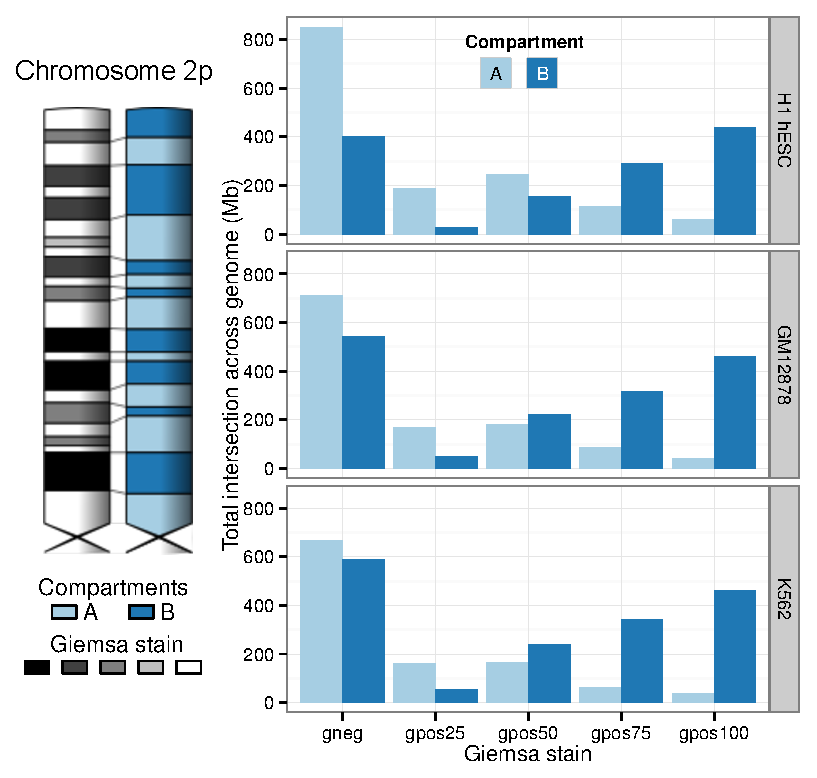
\includegraphics[width=.7\textwidth]{figs/gbands.pdf}
\captionsetup{width=\textwidth}
\caption[ Giemsa--stain bands correspond to A/B compartments.]{ {\bf Giemsa--stain bands correspond to A/B compartments.}
Placeholder
}\label{fig:gbands}
\end{center}
\end{figure} 

\begin{figure}
\begin{center} 
\makebox[\textwidth][c]{ 
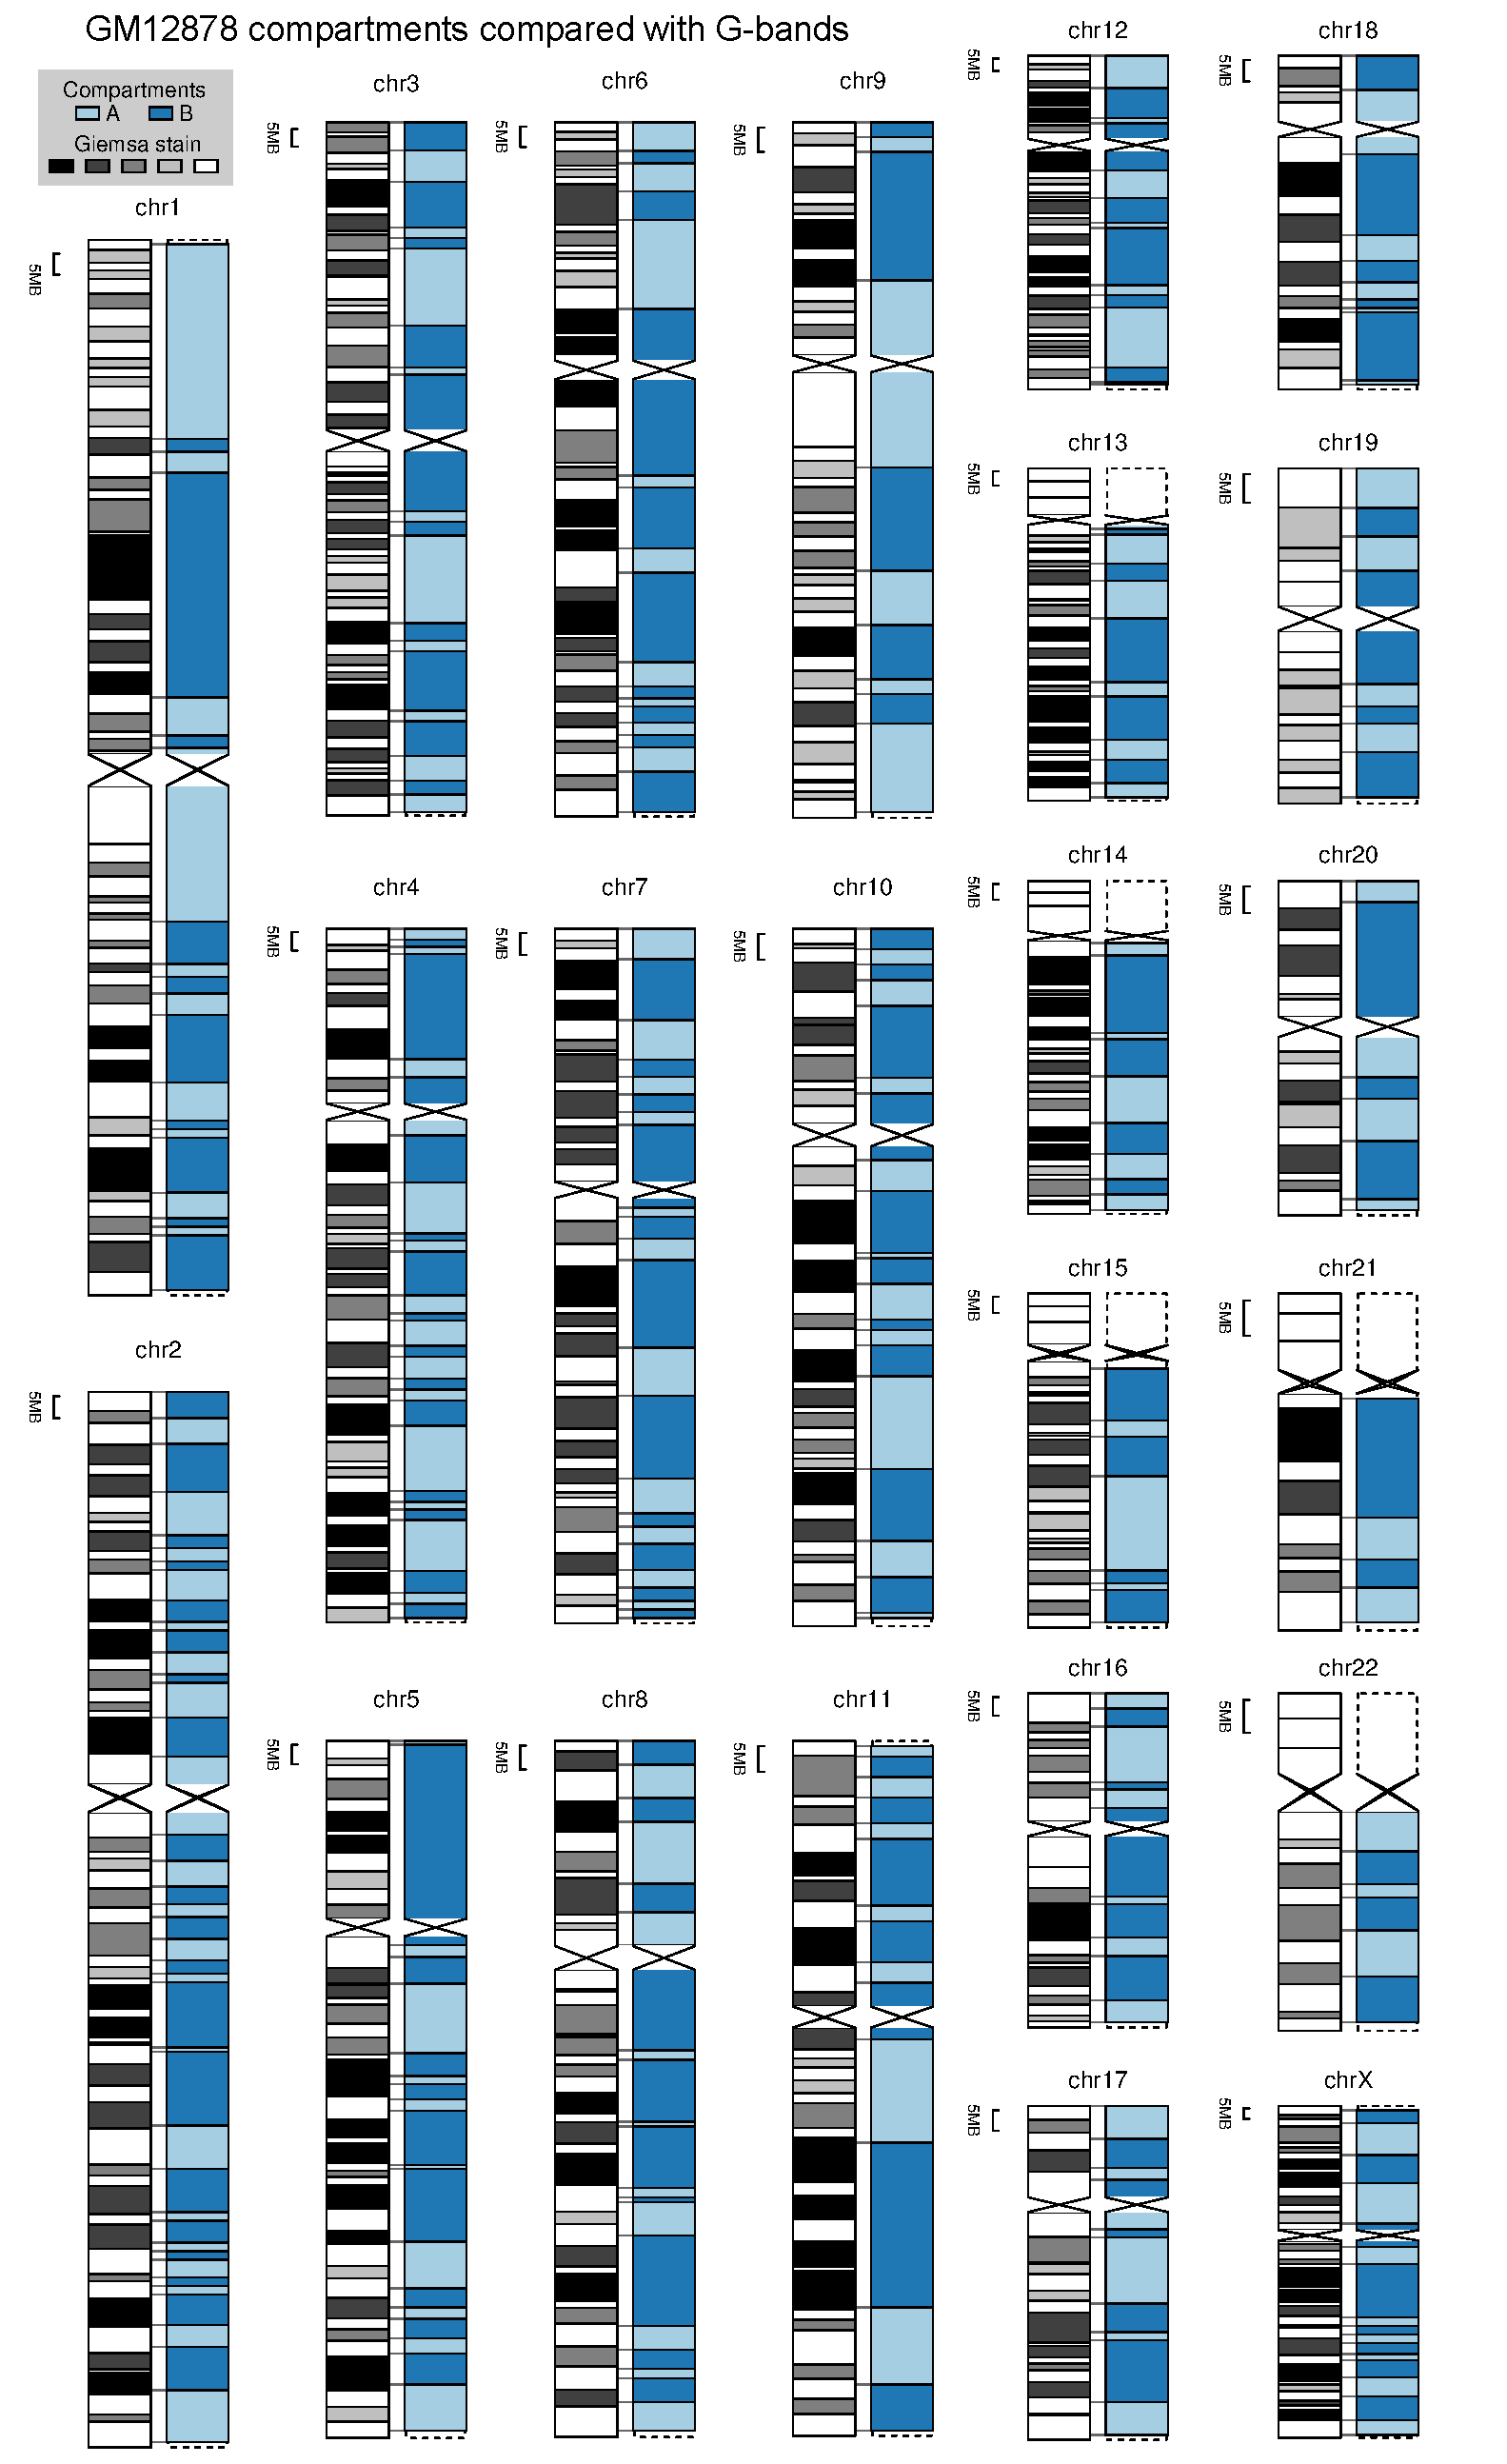
\includegraphics[width=1.2\textwidth]{figs/gb_ideo.pdf}
}
\captionsetup{width=\textwidth}
\caption[Genome-wide agreement between Giemsa bands and A/B compartments in the Gm12878 cell type.]{ {\bf Genome-wide agreement between Giemsa bands and A/B compartments in the Gm12878 cell type.}
Placeholder
}\label{fig:gbands2}
\end{center}
\end{figure} 

\subsection{Superboundaries}

Thus far compartment and TAD boundaries have been considered separately, however it is of interest to consider how these boundary regions interact across scales. Open questions remain about the co-occurence of these two boundary regions, and whether 


\ifstandalone
\begin{small}
\bibliography{/Users/benmoore/Documents/library,/Users/benmoore/Documents/customrefs}
\end{small}
\fi

\end{document}


% will this chapter be a goer?
%\input{5-comparative/comparative.tex}

\documentclass[a4paper,10pt,oneside]{book}

% packages 
\usepackage{arsclassica}    % fancy layout
\usepackage[english]{babel}\addto{\captionsenglish}{\renewcommand{\bibname}{References}}
\usepackage{caption}         % figure captions
\usepackage[square,numbers,super,sort&compress]{natbib}  % bibliography style
\usepackage[cc]{titlepic}    % enable logo on title page
\usepackage{graphicx}       % logo related

\usepackage{standalone}
\standalonetrue

% don't hang captions
\captionsetup{format=plain}

% bibliography
\bibliographystyle{../thesis}

% title setup
\title{ \vspace{3in} Unravelling higher order genome organisation {\small [working
    title]} \\ \vspace{2em} {\large {\bf Results 5: Collaborations}} }
\author{Benjamin L. Moore}
\titlepic{\vspace{2.2in} 
\includegraphics[width=\textwidth]{/Users/benmoore/hvl/1yrReport/figs/igmm.png}}

\begin{document}

%\maketitle

\chapter{Local chromatin conformation}

\section{Introduction}

The Hi-C assay provides a genome-wide overview of chromatin conformation, however this broad scope imposes resolution limits inherent to an all-vs-all assay. For a closer look at chromatin conformation within a region of interest, alternative C-based assays such as 3C, 4C and 5C can be employed alongside classical microscopy techniques like FISH.

Here I discuss two collaborative projects involving the use of 4C and 5C data to "zoom in" on two well-studied regions related to limb development: the ZRS enhancer and HoxD gene cluster.

\section{Chromatin conformation at the SHH locus}

\begin{figure}
\begin{center} 
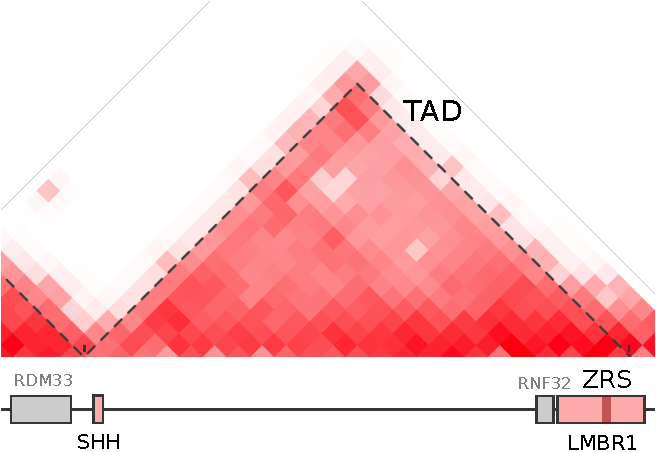
\includegraphics[width=.7\textwidth]{figs/shhtad.pdf}
\captionsetup{width=\textwidth} 
\caption[SHH--ZRS contacts occur within a stable TAD.]{ {\bf SHH--ZRS contacts occur within a stable TAD. }
An approximately 1 Mb region of the mouse genome is shown below a Hi-C contact map (derived from previously published data\cite{Dixon2012}). A clear TAD can be identified spanning from SHH to ZRS, dashed lines show TAD boundaries called by \citet{Dixon2012}. This figure was generated for \citet{Anderson2014a}.
}\label{fig:shhtad}
\end{center} 
\end{figure} 

Anterior-posterior patterning in the developing limb is regulated in mammals by \emph{Sonic hedgehog} (SHH).\cite{Anderson2012} Specifically, the SHH gene is expressed within a confined region named the "zone of polarising activity". Its expression within this region is known to be regulated by a well-studied enhancer, the "zone of polarising activity regulatory sequence" or ZRS.\cite{Hill2013a} ZRS is located almost 1 Mb downstream of its target SHH promoter in humans, and is located in intronic regions of another gene, LMBR1, and is conserved across mammals and fish (Fig. \ref{fig:shhtad}).\cite{Hill2013a, Laurell2012} Single point mutations and short insertions within this enhancer have been linked to various limb deformities, including pre- and post-axial polydactyly.\cite{Anderson2012, Lettice2008, Laurell2012} For example, a heritable point mutation in the ZRS enhancer is the cause of polydactyly in "Hemingway cats", a large group of domestic cats with extra toes that reside at the former home of Ernest Hemingway.\cite{Lettice2008}  

Collaborators have developed a model system which allows inducible SHH expression in a non-expressing 14fp cell line derived from the developing limb bud. Application of trichostatin A (TSA) then leads to detectable SHH expression, and increased levels of the histone activation mark H3K27ac at the ZRS (\emph{unpublished data}). However, the question remains whether this TSA treatment is fundamentally altering local chromatin structure, that is, bringing together the ZRS enhancer with its target SHH promoter, or whether ZRS and SHH are in contact in both the active and non-expressing cell lines and SHH expression is blocked through other means. Analysis of the region through FISH implies similar levels of compaction in SHH expressing and non-expressing cells (\emph{data not shown}), suggesting the latter explanation.

My part in this collaboration was to analyse 3C-seq (also known as 4C) data recorded by our collaborators for the SHH--ZRS region in mouse. Additionally, the 4C procedure\cite{Stadhouders2013} was adapted for specific in-house sequencing instruments (Ion Torrent Ion Proton\textsuperscript{TM} sequenced as opposed to Illumina\textsuperscript{TM} technology) and as such required diagnostics to confirm the experimental data was accurate. 

% Adam sent a powerpoint he gave for section meeting, see also Prof Hill's publications

\subsection{Analysis of ZRS interactions}

\begin{figure}
\begin{center} 
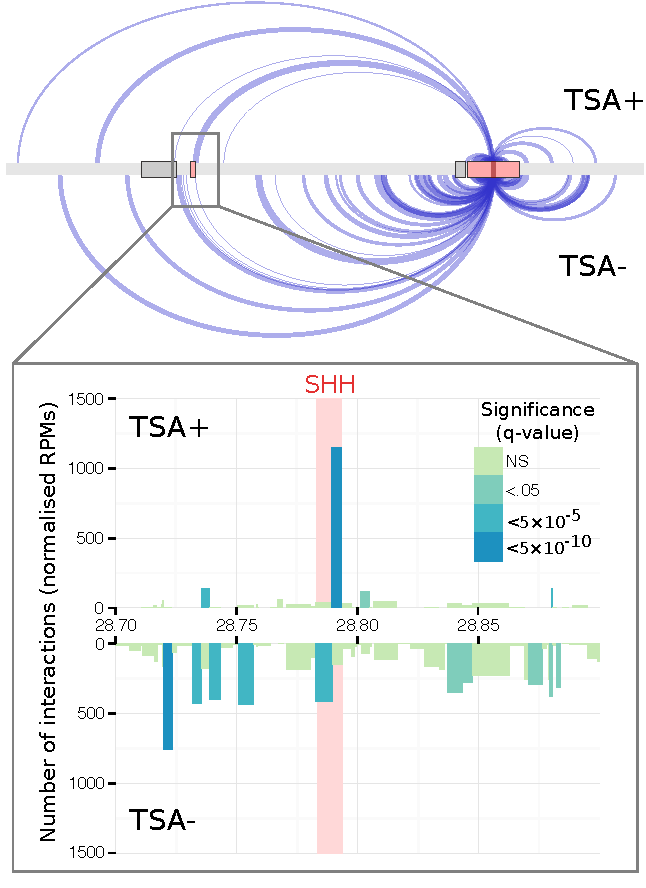
\includegraphics[width=.8\textwidth]{figs/shharc_full.pdf}
\captionsetup{width=\textwidth} 
\caption[TSA treatment induces a strong ZRS--SHH interaction. ]{ {\bf TSA treatment induces a strong ZRS--SHH interaction. }
4C interactions are shown as edges from source node (ZRS enhancer bait fragment) to targets along an approximately 2 Mb region of chromosome 5. Edge width is proportional to the number of interactions, only highly significant interactions are shown (FDR $q$-value $<5 \times 10 ^{-5}$). Zoomed region shows the number of interactions of the bait region with SHH in both treated and untreated samples. Each rectangle is a restriction fragment, coloured by FDR $q$-value indicating the significance of the interaction above expected levels.
}\label{fig:ssharc}
\end{center} 
\end{figure} 

4C experiments were performed by collaborators using the ZRS region as a bait sequence, or "viewpoint", such that it contacts were measured with all other HindIII restriction fragments genome-wide. 4C was performed in both untreated and non-SHH expressing cells (\emph{TSA--}) and in cells treated with TSA, thereby causing SHH expression (\emph{TSA+}). 

The first stage in analysing these contacts is to convert observed raw sequencing reads to normalised frequencies (Methods \ref{methods:4cnorm}), these normalised values are then assigned significance scores in the form of $q$-values, with the aim of finding those significantly over-represented relative to expectation (Methods \ref{methods:4csignif}).

% Conclusions: appears ZRS contacts become more targetted in TSA+ cells, before more diffuse. 
% Maybe in contact all the time (supported by FISH data) but not engaging in specific contacts when non-expressing.

\subsection{4C / Hi-C comparison}

Hi-C data in mouse cells has been previously published,\cite{Dixon2012} so can be compared with this novel 4C data to give broader contextual information about chromatin conformation in the region under study.

\subsection{Assay diagnostics}

The 4C protocol used by our collaborators in this work was that of \citet{Stadhouders2013}. In it, the authors advise some statistical tests to ensure the quality of the experiment results. Among these were:\cite{Stadhouders2013}

\begin{enumerate}
\item Sequencing reads should be found to have high duplication rates of $95\%$ or greater.
\item $50\%$ or more of all reads should map to the chromosome on which the bait region is located.
\end{enumerate}

\subsection{3D modelling with 5C data}

All-vs-all contacts measured either genome-wide in the case of Hi-C, or over a defined region with 5C, can be used to infer the trajectory of chromatin fibres in three-dimensions through a variety of methods (e.g. \cite{Hu2013a, Varoquaux2014a, Lesne2014, Trieu2014, Peng2013}). 5C data was generated over this same SHH--ZRS region (Fig. \ref{fig:shhtad}) with the aim of developing a multi-point perspective on local chromatin conformation beyond that available from 4C data.

We used this 5C experimental data in combination with a particular three-dimensional inference program  (\texttt{AutoChrom3D}\cite{Peng2013}) in an attempt to compare polymer trajectories in TSA treated and untreated 14fp mouse cells.

\section{5C in the HoxD region}

HoxD is another well-studied genetic system involved in limb development and under the control of known enhancers. In this experiment, our collaborators were interested in the chromatin conformations of HoxD13 loci in both the anterior and posterior developing limb bud, particularly how and where the two differed. To this end, our collaborators performed 5C for two biological replicates in anterior and posterior limb bud cell lines, and my contribution was to call differential contacts between the two conditions.

% files for this under iain on ext HD
% relevant publications: http://dev.biologists.org/content/139/17/3157.full.pdf+html

%Iain's thesis: https://www.era.lib.ed.ac.uk/handle/1842/8056

\subsection{Differential contacts}

% raw diff: fold change?

\begin{figure}
\begin{center} 
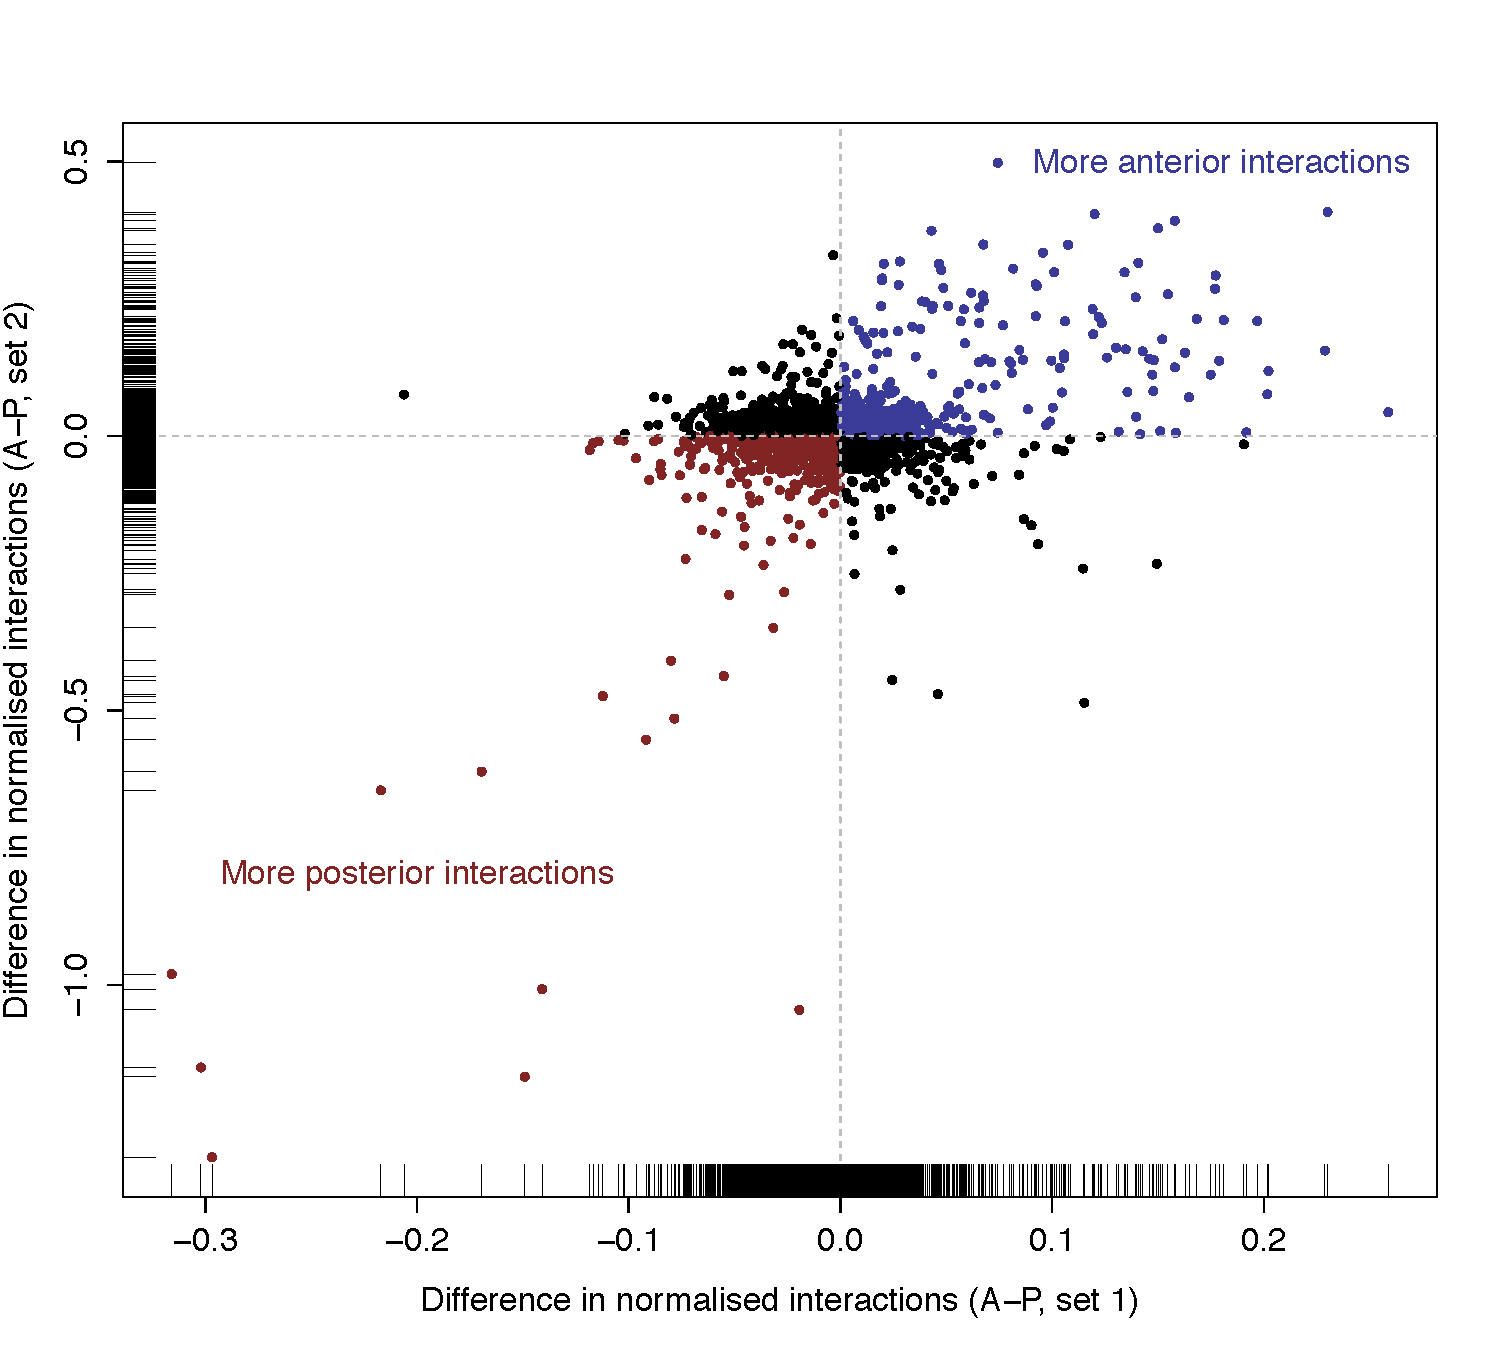
\includegraphics[width=\textwidth]{figs/5cfc.pdf}
\captionsetup{width=\textwidth} 
\caption[Raw differences between anterior and posterior 5C interactions.]{ {\bf Raw differences between anterior and posterior 5C interactions. }
Placeholder
}\label{fig:5cfc}
\end{center} 
\end{figure} 

% statistical test of differential contacts

\begin{figure}
\begin{center} 
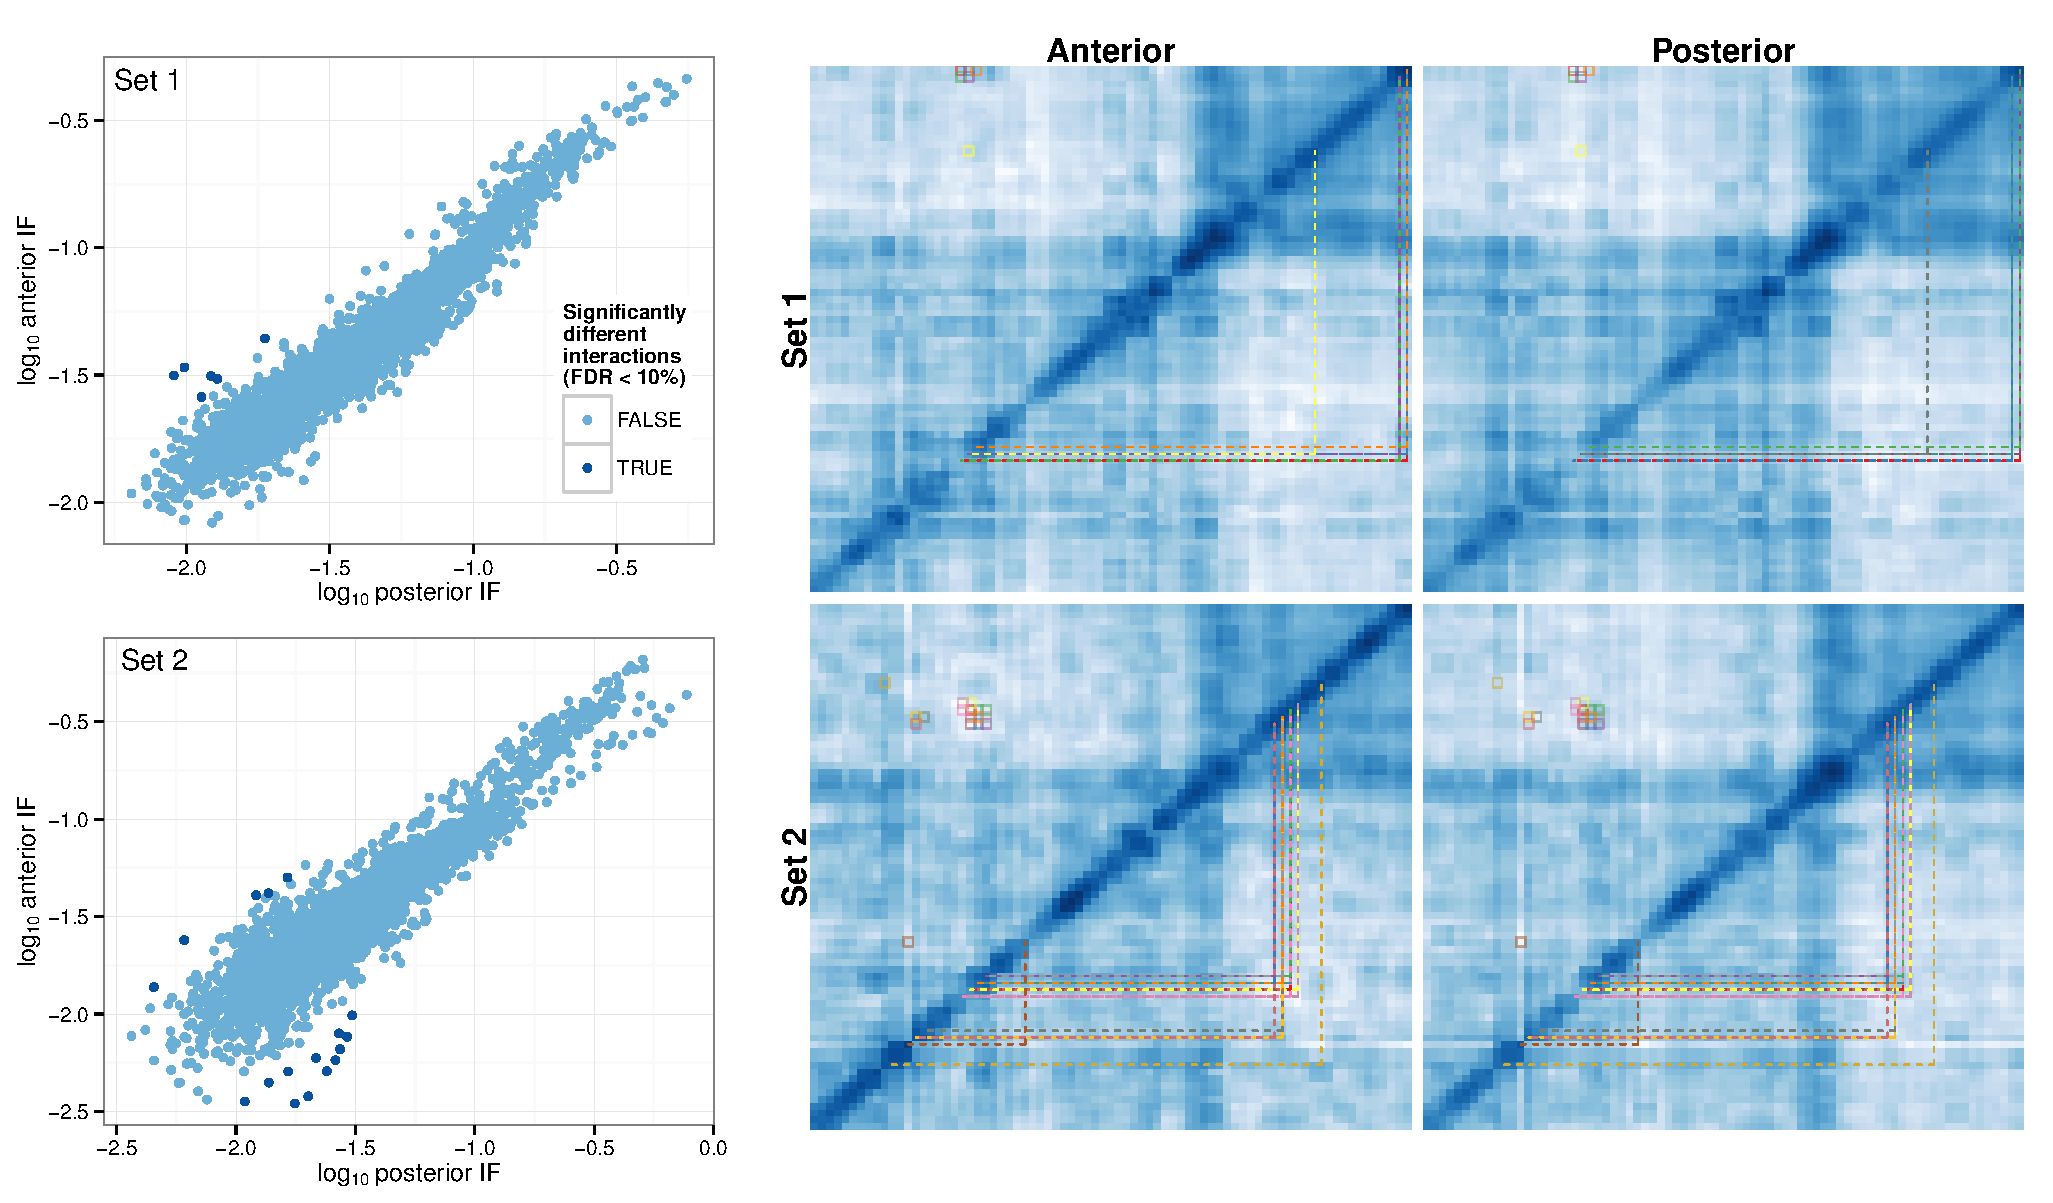
\includegraphics[width=\textwidth]{figs/5cdiff.pdf}
\captionsetup{width=\textwidth} 
\caption{ {\bf Will we use this stuff? }
Placeholder
}\label{fig:5cdiff}
\end{center} 
\end{figure} 


\subsection{5C / Hi-C comparison}

\begin{figure}
\begin{center} 
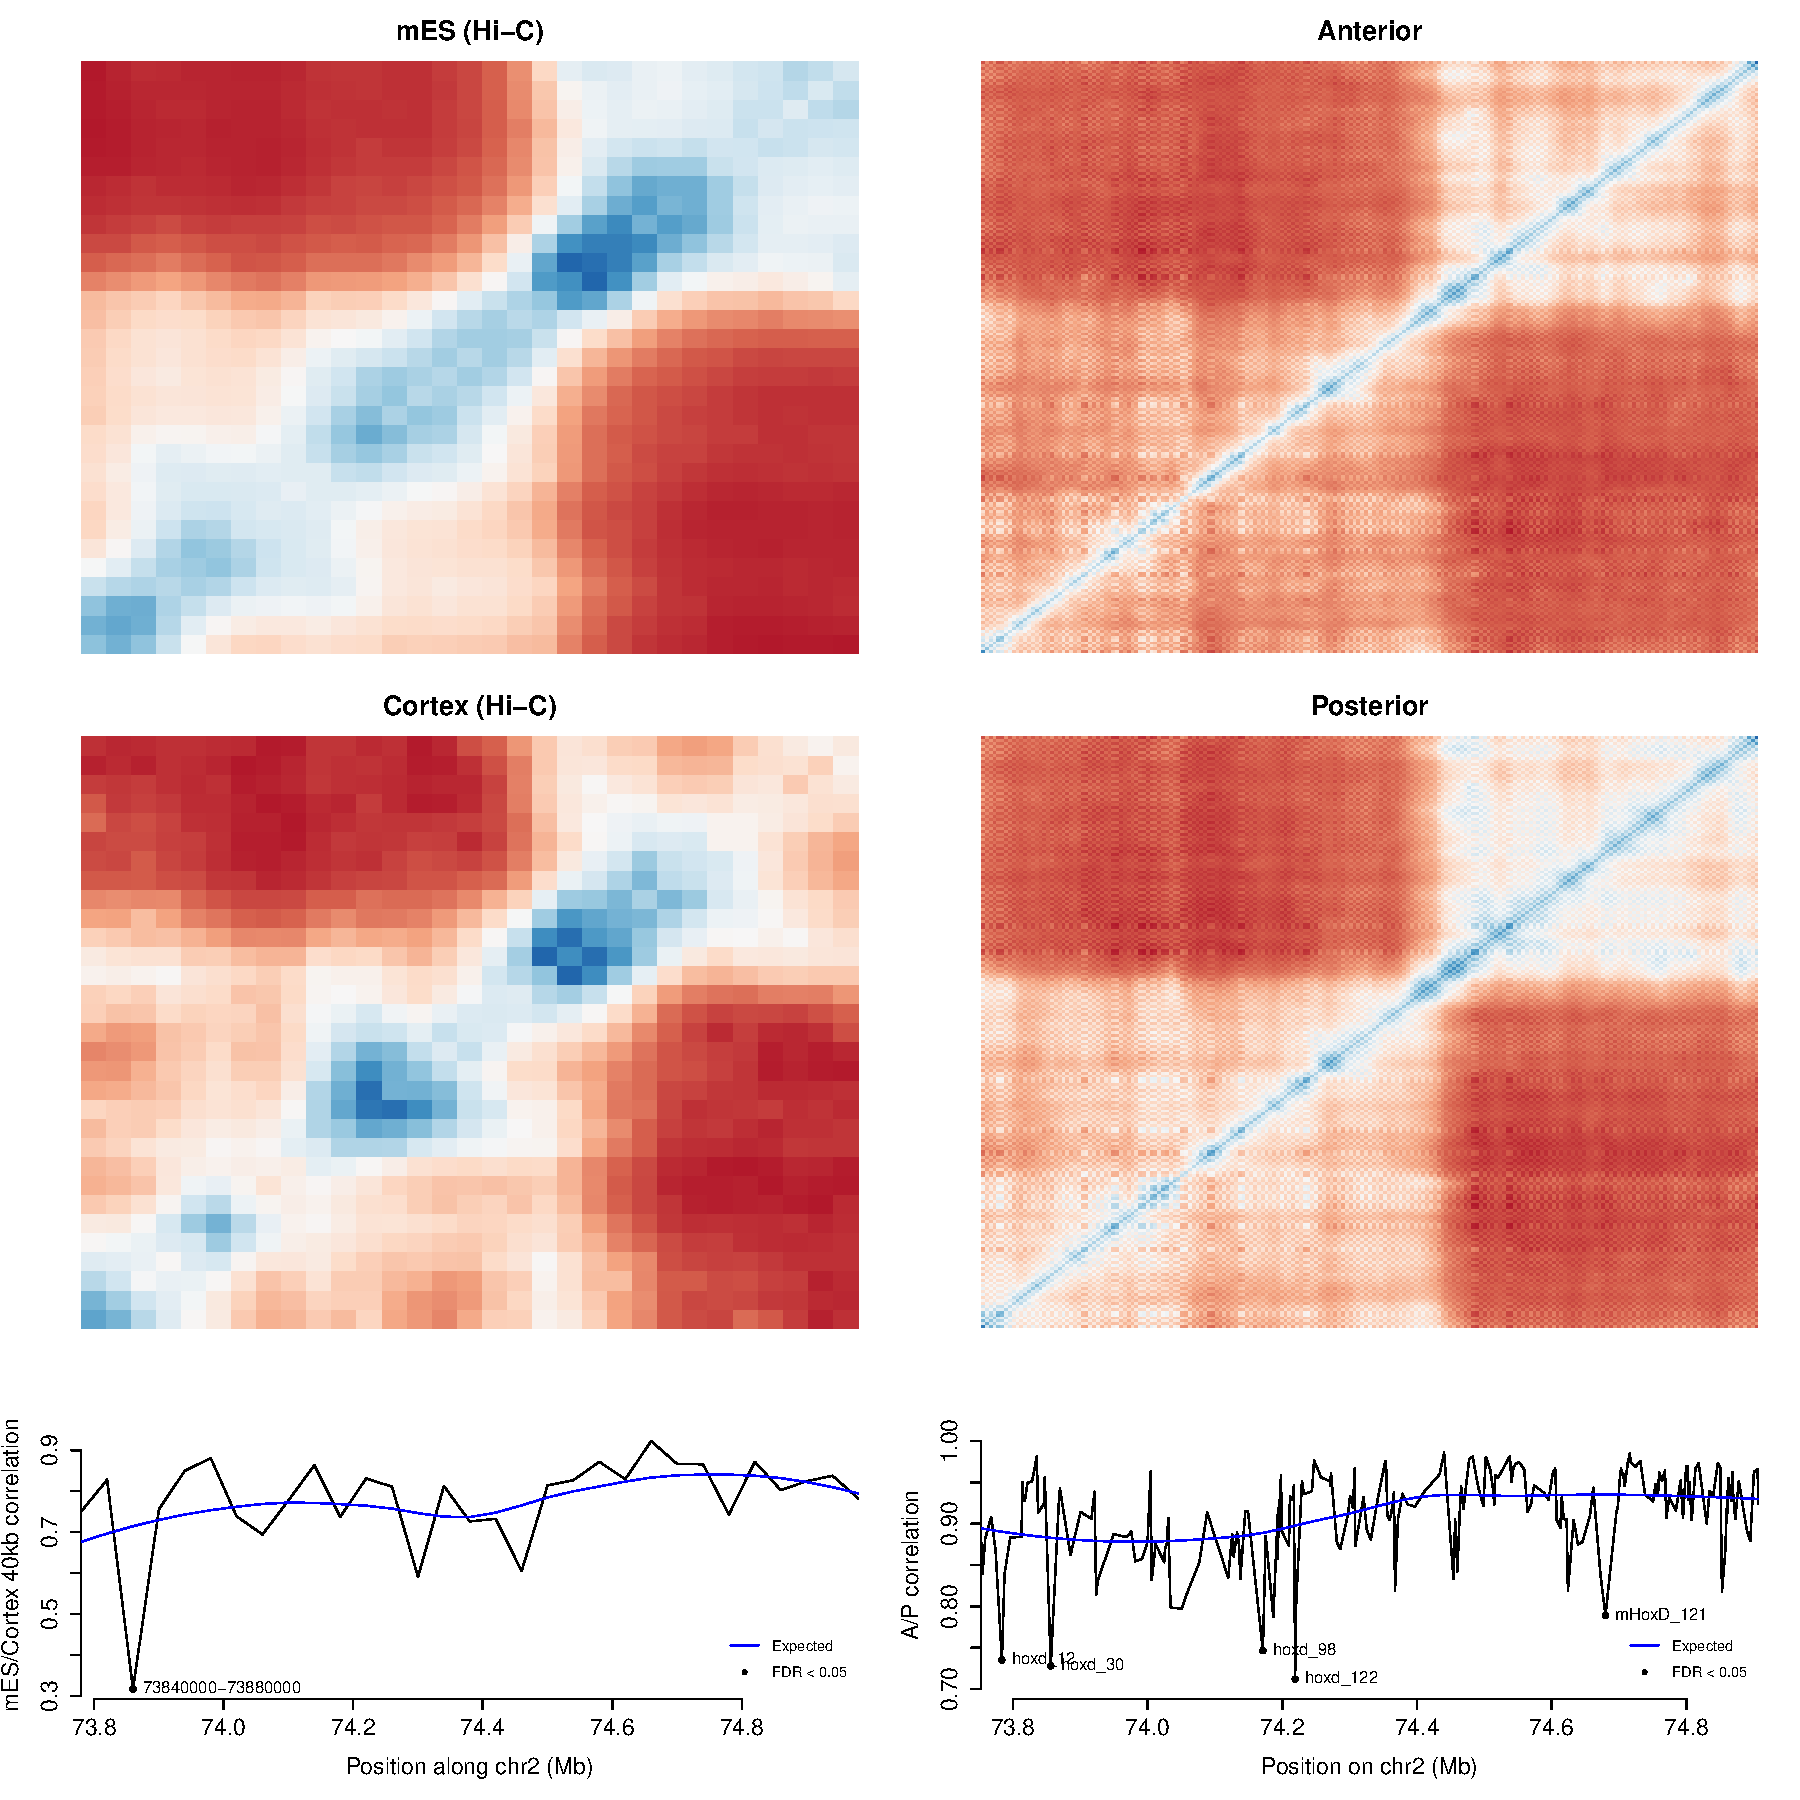
\includegraphics[width=\textwidth]{figs/5chic.pdf}
\captionsetup{width=\textwidth} 
\caption{ {\bf Will we use this stuff? }
Placeholder
}\label{fig:5cdiff}
\end{center} 
\end{figure} 


\ifstandalone
\begin{small}
\bibliography{/Users/benmoore/Documents/library,/Users/benmoore/Documents/customrefs}
\end{small}
\fi

\end{document}


% ---------- Discussion ---------- %
\documentclass[a4paper,10pt,oneside]{book}

% packages 
\usepackage{arsclassica}    % fancy layout
\usepackage[english]{babel}\addto{\captionsenglish}{\renewcommand{\bibname}{References}}
\usepackage{caption}         % figure captions
\usepackage[square,numbers,super,sort&compress]{natbib}  % bibliography style
\usepackage[cc]{titlepic}    % enable logo on title page
\usepackage{graphicx}       % logo related
\usepackage{standalone}

% bibliography
\bibliographystyle{../thesis}

% title setup
\title{ \vspace{3in} Unravelling higher order genome organisation {\small [working
    title]} \\ \vspace{2em} {\large {\bf Discussion}} }
\author{Benjamin L. Moore}
\titlepic{\vspace{2.2in} 
\includegraphics[width=\textwidth]{/Users/benmoore/hvl/1yrReport/figs/igmm.png}}

\begin{document}

\maketitle

\chapter{Discussion}

The recent abundance of epigenomic data in model cell types has
enabled accurate modelling of the transcriptional output of human
promoters, and a rigorously quantitative assessment of the most
influential chromatin features underlying gene expression
\cite{Dong2012}. We have shown that it is possible to construct
comparable models describing the features underlying higher order
chromatin structure, and that their predictive accuracy can be
high. Our analysis exploits Hi-C datasets that have been re-analysed,
from the intitial sequence read mapping onwards, identically for three
different cell types. These data were collated with 35 locus level
ENCODE chromatin datasets, also processed identically, and matched
across the same cell types. In common with previous studies
\cite{Chambers2013, Dixon2012}, we observed good concordance of higher
order chromatin structure, relected in Hi-C data, between different
cell types. Random forest models summarised the important
relationships among these many variables, providing insights into the
quantitative contributions of locus level chromatin features to higher
order structures. Although certain features were notably more
influential in a particular cell type, the models shared overlapping
constellations of informative features, allowing the cross application
of models between cell types.

Integrative analyses of locus level chromatin data have allowed the
prediction of functional chromatin states \cite{Ernst2012, Ram2011,
  Dunham2012, Hoffman2013} but these states typically emcompass small
regions such as the enhancers examined here. The prediction of higher
order chromatin domains has received much less attention, and it was
not clear until now that sufficient data existed to allow accurate
predictions. Our data show that accurate predictions of Hi-C derived
eigenvector values, and the nuclear compartment domains based upon
them, are entirely feasible. Strong and significant correlations are
seen between cell types for a variety of human higher order domains,
deliniating variation in replication timing, lamin association and
nuclear compartments derived from Hi-C eigenvectors
\cite{Chambers2013}. The data presented here therefore suggest that a
variety of such domains could be successfully modelled. Given the fact
that the binding patterns of most human chromatin components have not
yet been mapped the models presented here are remarkably successful,
though will undoubtedly improve with further data and algorithm
development. These models also allowed us to probe the features
underlying regions with variable higher order structure between cell
types, revealing enrichments of cell type specific enhancer activity,
and suggesting links between functional chromatin states and higher
order domain dynamics. It is not possible to distinguish cause and
effect using the current data, but it seems likely that the
alterations in domain organization occur prior to enhancer activity.

The current data suggest that the contributions of certain locus level
chromatin features to higher order structures vary between cell
types. Striking examples include the strong influence of H3K9me3 in
K562 leukemia cells, and EGR1 binding in H1 hESC. EGR1 is a pivotal
regulator of cell fate and mitogenesis with critical roles in
development and cancer \cite{Zwang2012}. While the patterns of
repressive H3K9me3 accumulation have been a focus in the cancer
literature and have been proposed as a diagnostic marker in leukemia
\cite{Muller-Tidow2010}. Similarly, the model for GM12878
(Epstein-Barr virus transformed lymphoblasoid) cells shows a
disproportionate influence of ATF3 binding patterns, and ATF3
induction is a known consequence of virus transformed cells
\cite{Hagmeyer1996}. Thus, the most cell type specific features in
these models may be important indicators of cell type specific
functions. These cell type specific features present a paradox, in
view of the strong correlations in organization genome wide across
different cell types \cite{Chambers2013, Dixon2012}, and the
demonstration that models trained in one cell type often perform well
with data from other cell types. These contradictory observations are
reconciled by the presence of inter-correlated clusters of features
underlying A and B compartments. The shifting membership of these
clusters evidently retains enough similarity between cell types to
enable the cross application of models.

Chromatin boundaries, separating TADs and nuclear compartments at
different scales, also showed cell type specific enrichments of
various locus level chromatin features. Across cell types, the
complexity of boundary composition varies considerably so that only a
few features were seen consistently enriched or depleted at
boundaries. Peaks associated with active promoters were notable for
both TAD and compartment boundaries in all cell types. Among the most
influentual variables for the random forest models constructed for the
two hematopoietic cell lines was the ubiquitous transcription factor
YY1, which re-appeared in the analysis of chromatin boundary
regions. Significant enrichments of YY1 were seen at TAD and nuclear
compartment boundaries in all three cell types. Thus, the same protein
was implicated at the level of broad genomic binding patterns (over 1
Mb intervals) and at the level of locally enriched peaks at boundary
regions (spanning 100-500 Kb). This is intriguing as YY1 has recently
been shown to co-localise with the architectural protein
CTCF \cite{Ong2014} and suggests that these proteins cooperate in the
establishment of domain boundaries. The identification of such
features, significantly enriched at boundary regions, provides
potential targets for deletion in experimental studies further
exploring the structure and function of domains
(e.g. \cite{Nora2012}). Both cell type specific and general
constituents of boundaries may have utility in the biomedical
interpretation of genomic variation in noncoding regions of the
genome.

\section{Conclusion}

It has become commonplace to discuss the multi-layered, hierarchical
organization of interphase chromosomes across strata ranging from
nuclear compartments, down to the spectra of histone modifications and
bound proteins at individual sub-genic regions. However we lack a
detailed understanding of how these strata interact. We have shown
that our perspectives of features occurring at different strata can be
bridged by modelling approaches, and the models produced can used to
explore the interrelationships between these different features
quantitatively. 

We constructed cell type specific models of nuclear
organization, as reflected in Hi-C derived eigenvector profiles, to
discover the most influential features underlying higher order
structures. We found open and closed compartments to be
well-correlated with combinatorial patterns of histone modifications
and DNA binding proteins, enabling accurate predictive models. These
models could be cross-applied successfully between cell types
highlighting constellations of common structural features associated
with different nuclear compartments as expected. Dissection of the
most influential variables also revealed important differences between
models, consistent with the known biological contrasts among these
cell types, such as the prominence of EGR1 in embryonic stem cells and
H3K9me3 in the leukaemia cell line. Investigation of regions showing
variable nuclear organization across the three cell types under study,
revealed enrichments for cell type specific enhancer activity, often
nucleated at genes with known roles in cell type specific
functions. Finally we used model predictions to examine boundary
composition between higher order domains across cell types. Among
enrichments of a large number of factors observed at different
boundaries in different cell types, CTCF and YY1 were found
consistently and may cooperate to establish domain boundaries. In
summary, we show that integrative modelling of large chromatin dataset
collections using random forests can generate useful insights into
chromosome structure and seed testable hypotheses for further
experimental studies.

\ifstandalone
\begin{small}
\bibliography{/Users/benmoore/Documents/library,/Users/benmoore/Documents/customrefs}
\end{small}
\fi

\end{document}


\backmatter

% Appendix with includes
\documentclass[a4paper,11pt,oneside]{book}

% packages 
\usepackage{arsclassica}    % fancy layout
\usepackage[english]{babel}\addto{\captionsenglish}{\renewcommand{\bibname}{References}}
\usepackage{caption}         % figure captions
\usepackage[square,numbers,super,sort&compress]{natbib}  % bibliography style
\usepackage[cc]{titlepic}    % enable logo on title page
\usepackage{graphicx}       % logo related
\usepackage{pdfpages}

\usepackage{standalone}
\standalonetrue

% GO term margins 
\usepackage{longtable}
\usepackage{geometry}

% bibliography
\bibliographystyle{../thesis}

% title setup
\title{ \vspace{3in} Unravelling higher order genome organisation {\small [working
    title]} \\ \vspace{2em} {\large {\bf Results 5: Collaborations}} }
\author{Benjamin L. Moore}
\titlepic{\vspace{2.2in} 
\includegraphics[width=\textwidth]{/Users/benmoore/hvl/1yrReport/figs/igmm.png}}

\begin{document}


\chapter{Appendices}

% GO term tables
\setcounter{table}{0}
\makeatletter 
\renewcommand{\thetable}{A\@arabic\c@table}
\makeatother

\newgeometry{left=2cm,right=2cm}

{\tiny 
\begin{longtable}{lllllll}
\caption[Gm12878 functional enrichments in regions of variable structure.]{
{\bf 
Gm12878 functional enrichments in regions of variable structure.
} FE: fold enrichment; FDR: false discovery rate.
}\label{tab:gmgo}\\
\endfirsthead
Category          & Term                                          &
Count & \%   & FE & $p$-value   & FDR      \\
GOTERM\_CC\_FAT   & GO:0005882~intermediate filament              & 36    & 4.20 & 4.90            & 6.42E-15 & 8.95E-12 \\
GOTERM\_CC\_FAT   & GO:0045111~intermediate filament cytoskeleton & 36    & 4.20 & 4.79            & 1.35E-14 & 1.87E-11 \\
SP\_PIR\_KEYWORDS & keratin                                       & 31    & 3.62 & 5.64            & 1.72E-14 & 2.47E-11 \\
INTERPRO          & IPR007951:PMG                                 & 11    & 1.28 & 25.11           & 9.80E-14 & 1.56E-10
\end{longtable}
}

\clearpage

{\scriptsize 
\begin{longtable}{lllllll}
\caption[H1 hESC functional enrichments in regions of variable structure.]{ {\bf
H1 hESC functional enrichments in regions of variable structure. }
FE: fold enrichment; FDR: false discovery rate.
}\label{tab:h1go}\\
\endfirsthead

Category          & Term
& Count & \%    & FE & $p$-value   & FDR      \\
PIR\_SUPERFAMILY  & PIRSF003152:G protein-coupled olfactory receptor, class II      & 116   & 10.55 & 6.64            & 3.25E-68 & 4.41E-65 \\
INTERPRO          & IPR000725:Olfactory receptor                                    & 116   & 10.55 & 6.53            & 7.58E-63 & 1.21E-59 \\
SP\_PIR\_KEYWORDS & olfaction                                                       & 116   & 10.55 & 6.40            & 2.07E-61 & 2.97E-58 \\
GOTERM\_MF\_FAT   & GO:0004984~olfactory receptor activity                          & 116   & 10.55 & 6.13            & 1.30E-60 & 1.97E-57 \\
GOTERM\_BP\_FAT   & GO:0007608~sensory perception of smell                          & 117   & 10.64 & 5.96            & 1.91E-59 & 3.35E-56 \\
GOTERM\_BP\_FAT   & GO:0007606~sensory perception of chemical stimulus              & 118   & 10.73 & 5.37            & 1.71E-54 & 3.01E-51 \\
KEGG\_PATHWAY     & hsa04740:Olfactory transduction                                 & 108   & 9.82  & 4.94            & 8.72E-51 & 1.03E-47 \\
SP\_PIR\_KEYWORDS & sensory transduction                                            & 125   & 11.36 & 4.58            & 2.61E-48 & 3.74E-45 \\
INTERPRO          & IPR017452:GPCR, rhodopsin-like superfamily                      & 131   & 11.91 & 4.03            & 1.40E-44 & 2.24E-41 \\
INTERPRO          & IPR000276:7TM GPCR, rhodopsin-like                              & 131   & 11.91 & 4.02            & 1.68E-44 & 2.68E-41 \\
PIR\_SUPERFAMILY  & PIRSF800006:rhodopsin-like G protein-coupled receptors          & 131   & 11.91 & 3.63            & 5.04E-43 & 6.85E-40 \\
GOTERM\_BP\_FAT   & GO:0007600~sensory perception                                   & 138   & 12.55 & 3.54            & 4.78E-41 & 8.40E-38 \\
SP\_PIR\_KEYWORDS & g-protein coupled receptor                                      & 136   & 12.36 & 3.62            & 1.69E-40 & 2.42E-37 \\
GOTERM\_BP\_FAT   & GO:0050890~cognition                                            & 143   & 13.00 & 3.23            & 5.34E-38 & 9.38E-35 \\
SP\_PIR\_KEYWORDS & transducer                                                      & 137   & 12.45 & 3.39            & 1.48E-37 & 2.12E-34 \\
GOTERM\_BP\_FAT   & GO:0050877~neurological system process                          & 163   & 14.82 & 2.72            & 3.85E-34 & 6.76E-31 \\
GOTERM\_BP\_FAT   & GO:0007186~G-protein coupled receptor protein signaling pathway & 148   & 13.45 & 2.77            & 1.36E-31 & 2.40E-28 \\
SP\_PIR\_KEYWORDS & receptor                                                        & 172   & 15.64 & 2.31            & 3.72E-26 & 5.33E-23 \\
GOTERM\_BP\_FAT   & GO:0007166~cell surface receptor linked signal transduction     & 188   & 17.09 & 2.06            & 8.02E-24 & 1.41E-20 \\
SP\_PIR\_KEYWORDS & cell membrane                                                   & 198   & 18.00 & 1.86            & 5.96E-19 & 8.52E-16 \\
UP\_SEQ\_FEATURE  & topological domain:Extracellular                                & 227   & 20.64 & 1.72            & 1.26E-17 & 2.20E-14 \\
UP\_SEQ\_FEATURE  & topological domain:Cytoplasmic                                  & 250   & 22.73 & 1.52            & 1.13E-12 & 1.98E-09 \\
UP\_SEQ\_FEATURE  & disulfide bond                                                  & 211   & 19.18 & 1.56            & 9.11E-12 & 1.60E-08 \\
SP\_PIR\_KEYWORDS & disulfide bond                                                  & 214   & 19.45 & 1.52            & 6.20E-11 & 8.88E-08 \\
UP\_SEQ\_FEATURE  & glycosylation site:N-linked (GlcNAc...)                         & 285   & 25.91 & 1.41            & 7.31E-11 & 1.28E-07 \\
GOTERM\_CC\_FAT   & GO:0005886~plasma membrane                                      & 255   & 23.18 & 1.37            & 1.26E-09 & 1.77E-06 \\
SP\_PIR\_KEYWORDS & glycoprotein                                                    & 289   & 26.27 & 1.37            & 1.83E-09 & 2.61E-06 \\
GOTERM\_CC\_FAT   & GO:0016021~integral to membrane                                 & 328   & 29.82 & 1.27            & 9.34E-09 & 1.31E-05 \\
SP\_PIR\_KEYWORDS & transmembrane                                                   & 317   & 28.82 & 1.31            & 1.37E-08 & 1.96E-05 \\
UP\_SEQ\_FEATURE  & transmembrane region                                            & 314   & 28.55 & 1.31            & 2.03E-08 & 3.56E-05 \\
GOTERM\_CC\_FAT   & GO:0031224~intrinsic to membrane                                & 333   & 30.27 & 1.24            & 7.49E-08 & 1.05E-04 \\
SMART             & SM00355:ZnF\_C2H2                                               & 69    & 6.27  & 1.86            & 4.23E-07 & 5.43E-04 \\
UP\_SEQ\_FEATURE  & zinc finger region:C2H2-type 5                                  & 55    & 5.00  & 2.08            & 5.12E-07 & 8.99E-04 \\
UP\_SEQ\_FEATURE  & zinc finger region:C2H2-type 4                                  & 57    & 5.18  & 2.01            & 8.49E-07 & 0.0015   \\
INTERPRO          & IPR013087:Zinc finger, C2H2-type/integrase, DNA-binding         & 59    & 5.36  & 1.94            & 1.73E-06 & 0.0028   \\
UP\_SEQ\_FEATURE  & zinc finger region:C2H2-type 2                                  & 58    & 5.27  & 1.95            & 1.73E-06 & 0.0030   \\
SP\_PIR\_KEYWORDS & membrane                                                        & 372   & 33.82 & 1.21            & 2.69E-06 & 0.0038   \\
INTERPRO          & IPR015880:Zinc finger, C2H2-like                                & 69    & 6.27  & 1.78            & 4.09E-06 & 0.0065   \\
UP\_SEQ\_FEATURE  & zinc finger region:C2H2-type 8                                  & 44    & 4.00  & 2.14            & 4.13E-06 & 0.0073   \\
UP\_SEQ\_FEATURE  & zinc finger region:C2H2-type 3                                  & 58    & 5.27  & 1.90            & 4.43E-06 & 0.0078   \\
UP\_SEQ\_FEATURE  & zinc finger region:C2H2-type 7                                  & 46    & 4.18  & 2.06            & 5.87E-06 & 0.0103   \\
INTERPRO          & IPR007087:Zinc finger, C2H2-type                                & 67    & 6.09  & 1.75            & 9.19E-06 & 0.0147   \\
UP\_SEQ\_FEATURE  & zinc finger region:C2H2-type 6                                  & 48    & 4.36  & 1.99            & 9.83E-06 & 0.0173  
\end{longtable}
}

\clearpage

{\scriptsize 
\begin{longtable}{lllllll}
\caption[K562 functional enrichments in regions of variable structure.]{
{\bf K562 functional enrichments in regions of variable structure. }
FE: fold enrichment; FDR: false discovery rate.
}\label{tab:k5go}\\
\endfirsthead

%\begin{tabular}
Category          & Term
& Count & \%    & FE & $p$-value   & FDR      \\
PIR\_SUPERFAMILY  & PIRSF038651:G protein-coupled olfactory receptor, class I       & 26    & 7.08  & 24.94           & 7.86E-30 & 8.99E-27 \\
GOTERM\_MF\_FAT   & GO:0004984~olfactory receptor activity                          & 40    & 10.90 & 6.12            & 7.39E-20 & 1.01E-16 \\
INTERPRO          & IPR000725:Olfactory receptor                                    & 39    & 10.63 & 6.18            & 3.00E-19 & 4.29E-16 \\
SP\_PIR\_KEYWORDS & olfaction                                                       & 39    & 10.63 & 6.15            & 4.55E-19 & 6.09E-16 \\
GOTERM\_BP\_FAT   & GO:0007608~sensory perception of smell                          & 39    & 10.63 & 5.48            & 1.19E-17 & 1.94E-14 \\
SP\_PIR\_KEYWORDS & sensory transduction                                            & 44    & 11.99 & 4.60            & 8.72E-17 & 1.44E-13 \\
GOTERM\_BP\_FAT   & GO:0007606~sensory perception of chemical stimulus              & 39    & 10.63 & 4.89            & 6.32E-16 & 1.09E-12 \\
KEGG\_PATHWAY     & hsa04740:Olfactory transduction                                 & 38    & 10.35 & 4.58            & 6.87E-16 & 7.22E-13 \\
INTERPRO          & IPR017452:GPCR, rhodopsin-like superfamily                      & 43    & 11.72 & 3.72            & 2.96E-13 & 4.23E-10 \\
INTERPRO          & IPR000276:7TM GPCR, rhodopsin-like                              & 43    & 11.72 & 3.72            & 3.10E-13 & 4.43E-10 \\
SP\_PIR\_KEYWORDS & transducer                                                      & 46    & 12.53 & 3.26            & 4.97E-12 & 6.65E-09 \\
SP\_PIR\_KEYWORDS & g-protein coupled receptor                                      & 44    & 11.99 & 3.35            & 6.34E-12 & 8.48E-09 \\
PIR\_SUPERFAMILY  & PIRSF800006:rhodopsin-like G protein-coupled receptors          & 42    & 11.44 & 3.26            & 6.34E-12 & 7.26E-09 \\
GOTERM\_BP\_FAT   & GO:0007600~sensory perception                                   & 45    & 12.26 & 3.18            & 1.10E-11 & 1.80E-08 \\
GOTERM\_BP\_FAT   & GO:0050890~cognition                                            & 46    & 12.53 & 2.87            & 1.87E-10 & 3.07E-07 \\
UP\_SEQ\_FEATURE  & zinc finger region:C2H2-type 10                                 & 27    & 7.36  & 4.64            & 1.94E-10 & 3.10E-07 \\
UP\_SEQ\_FEATURE  & zinc finger region:C2H2-type 1; degenerate                      & 17    & 4.63  & 8.23            & 2.35E-10 & 3.77E-07 \\
GOTERM\_BP\_FAT   & GO:0007186~G-protein coupled receptor protein signaling pathway & 51    & 13.90 & 2.63            & 2.87E-10 & 4.70E-07 \\
UP\_SEQ\_FEATURE  & zinc finger region:C2H2-type 11                                 & 25    & 6.81  & 4.91            & 3.32E-10 & 5.31E-07 \\
UP\_SEQ\_FEATURE  & zinc finger region:C2H2-type 9                                  & 28    & 7.63  & 4.30            & 4.58E-10 & 7.33E-07 \\
UP\_SEQ\_FEATURE  & zinc finger region:C2H2-type 12                                 & 23    & 6.27  & 5.27            & 5.15E-10 & 8.24E-07 \\
SMART             & SM00349:KRAB                                                    & 26    & 7.08  & 4.36            & 7.67E-10 & 8.65E-07 \\
UP\_SEQ\_FEATURE  & zinc finger region:C2H2-type 15                                 & 17    & 4.63  & 7.40            & 1.17E-09 & 1.88E-06 \\
UP\_SEQ\_FEATURE  & zinc finger region:C2H2-type 7                                  & 30    & 8.17  & 3.84            & 1.33E-09 & 2.13E-06 \\
INTERPRO          & IPR001909:Krueppel-associated  box                              & 26    & 7.08  & 4.20            & 3.15E-09 & 4.49E-06 \\
UP\_SEQ\_FEATURE  & domain:KRAB                                                     & 25    & 6.81  & 4.37            & 3.38E-09 & 5.41E-06 \\
UP\_SEQ\_FEATURE  & zinc finger region:C2H2-type 14                                 & 17    & 4.63  & 6.32            & 1.19E-08 & 1.90E-05 \\
UP\_SEQ\_FEATURE  & zinc finger region:C2H2-type 13                                 & 19    & 5.18  & 5.50            & 1.19E-08 & 1.91E-05 \\
UP\_SEQ\_FEATURE  & zinc finger region:C2H2-type 8                                  & 27    & 7.36  & 3.73            & 1.86E-08 & 2.98E-05 \\
UP\_SEQ\_FEATURE  & zinc finger region:C2H2-type 6                                  & 29    & 7.90  & 3.42            & 3.22E-08 & 5.15E-05 \\
INTERPRO          & IPR001089:Small chemokine, C-X-C                                & 7     & 1.91  & 29.85           & 4.94E-08 & 7.06E-05 \\
INTERPRO          & IPR002473:Small chemokine, C-X-C/Interleukin 8                  & 7     & 1.91  & 27.72           & 8.52E-08 & 1.22E-04 \\
GOTERM\_BP\_FAT   & GO:0050877~neurological system process                          & 48    & 13.08 & 2.21            & 2.61E-07 & 4.27E-04 \\
INTERPRO          & IPR018048:Small chemokine, C-X-C, conserved site                & 7     & 1.91  & 22.83           & 3.35E-07 & 4.79E-04 \\
INTERPRO          & IPR002337:Haemoglobin, beta                                     & 5     & 1.36  & 55.44           & 5.04E-07 & 7.20E-04 \\
INTERPRO          & IPR013087:Zinc finger, C2H2-type/integrase, DNA-binding         & 30    & 8.17  & 2.77            & 1.34E-06 & 0.002    \\
SMART             & SM00355:ZnF\_C2H2                                               & 33    & 8.99  & 2.48            & 1.77E-06 & 0.002    \\
SP\_PIR\_KEYWORDS & receptor                                                        & 52    & 14.17 & 2.00            & 2.39E-06 & 0.003    \\
UP\_SEQ\_FEATURE  & zinc finger region:C2H2-type 5                                  & 27    & 7.36  & 2.90            & 2.39E-06 & 0.004    \\
UP\_SEQ\_FEATURE  & zinc finger region:C2H2-type 3                                  & 29    & 7.90  & 2.70            & 3.79E-06 & 0.006    \\
GOTERM\_MF\_FAT   & GO:0047760~butyrate-CoA ligase activity                         & 5     & 1.36  & 38.47           & 3.81E-06 & 0.005    \\
INTERPRO          & IPR007087:Zinc finger, C2H2-type                                & 33    & 8.99  & 2.43            & 5.58E-06 & 0.008    \\
PIR\_SUPERFAMILY  & PIRSF002522:CXC chemokine                                       & 6     & 1.63  & 20.55           & 6.13E-06 & 0.007    \\
SP\_PIR\_KEYWORDS & oxygen carrier                                                  & 5     & 1.36  & 35.19           & 6.39E-06 & 0.009    \\
INTERPRO          & IPR015880:Zinc finger, C2H2-like                                & 33    & 8.99  & 2.39            & 7.71E-06 & 0.011    \\
GOTERM\_BP\_FAT   & GO:0007166~cell surface receptor linked signal transduction     & 59    & 16.08 & 1.78            & 9.41E-06 & 0.015    \\
UP\_SEQ\_FEATURE  & zinc finger region:C2H2-type 16                                 & 11    & 3.00  & 6.18            & 1.14E-05 & 0.018    \\
PIR\_SUPERFAMILY  & PIRSF500045:hemoglobin, vertebrate type                         & 5     & 1.36  & 29.97           & 1.16E-05 & 0.013    \\
UP\_SEQ\_FEATURE  & zinc finger region:C2H2-type 17                                 & 10    & 2.72  & 7.02            & 1.20E-05 & 0.019    \\
UP\_SEQ\_FEATURE  & disulfide bond                                                  & 77    & 20.98 & 1.62            & 1.27E-05 & 0.020    \\
UP\_SEQ\_FEATURE  & topological domain:Extracellular                                & 75    & 20.44 & 1.62            & 1.99E-05 & 0.032    \\
PIR\_SUPERFAMILY  & PIRSF005559:zinc finger protein ZFP-36                          & 13    & 3.54  & 4.58            & 2.22E-05 & 0.025    \\
SP\_PIR\_KEYWORDS & disulfide bond                                                  & 78    & 21.25 & 1.59            & 2.44E-05 & 0.033    \\
UP\_SEQ\_FEATURE  & zinc finger region:C2H2-type 20                                 & 7     & 1.91  & 11.56           & 2.64E-05 & 0.042    \\
SP\_PIR\_KEYWORDS & blood                                                           & 5     & 1.36  & 25.59           & 2.89E-05 & 0.039    \\
SP\_PIR\_KEYWORDS & cell membrane                                                   & 63    & 17.17 & 1.70            & 3.07E-05 & 0.041   
%\end{tabular}

\end{longtable}
}

\restoregeometry

% paper
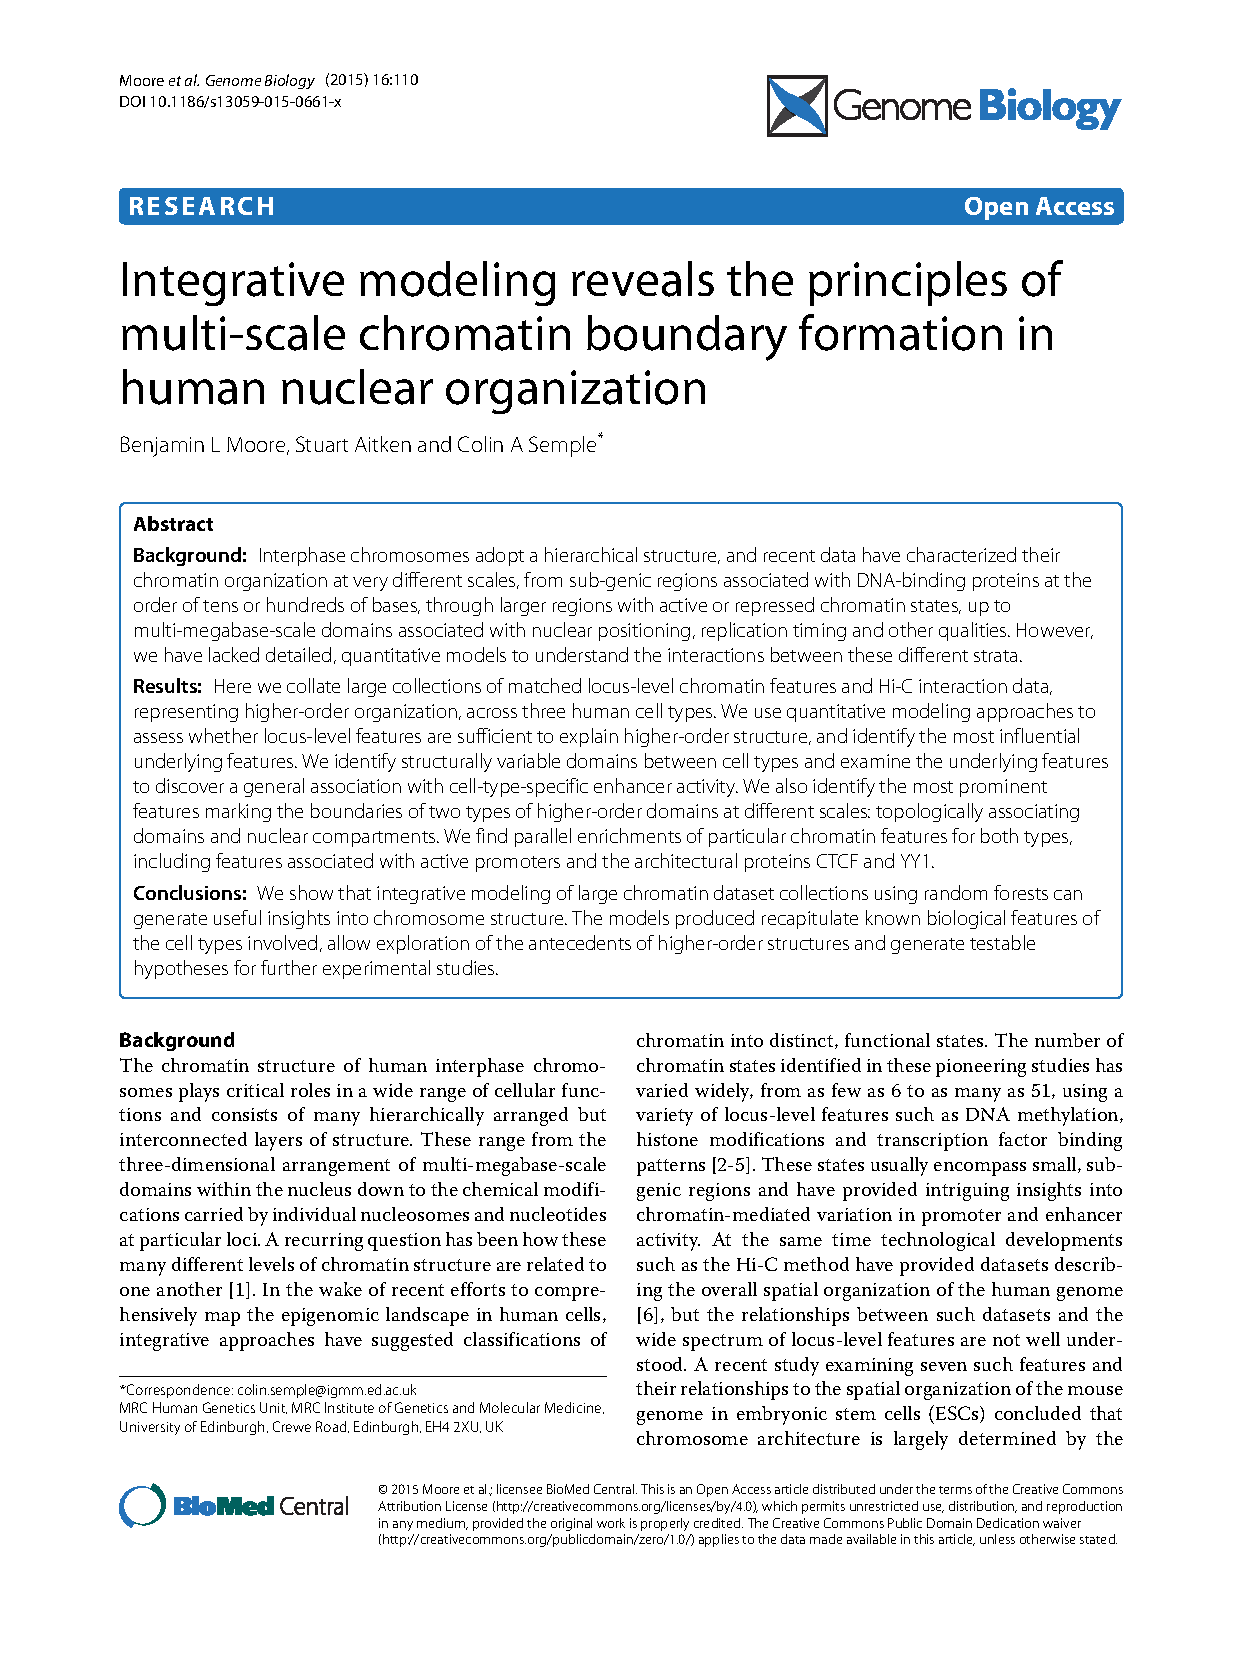
\includepdf[pages=-]{figs/genome_biol.pdf}


\ifstandalone
\begin{small}
\bibliography{/Users/benmoore/Documents/library,/Users/benmoore/Documents/customrefs}
\end{small}
\fi

\end{document}


% References (grabbed from includes)
%\begin{small}
\addcontentsline{toc}{chapter}{\sffamily\textls[80]{\scshape references}}
\bibliography{/Users/benmoore/Documents/library,/Users/benmoore/Documents/customrefs}
%\end{small}

\end{document}
